%%% File encoding: UTF-8
%% äöüÄÖÜß  <-- no German Umlauts here? Use an UTF-8 compatible editor!

%%% Magic comments for setting the correct parameters in compatible IDEs
% !TeX encoding = utf8
% !TeX program = pdflatex 
% !TeX spellcheck = en_US
% !BIB program = biber

\documentclass[master,english]{hgbthesis}
% Permissible options in [..]: 
%   Type of work: diploma, master (default), bachelor, internship 
%   Main language: german, english (default)
%%%----------------------------------------------------------

\RequirePackage[utf8]{inputenc}		% Remove when using lualatex or xelatex entfernen!

\graphicspath{{images/}}    % location of images and graphics
\logofile{logo}				% logo file = images/logo.pdf (use \logofile{} for no logo)
\bibliography{references}  	% name of bibliography file (references.bib)

%%%----------------------------------------------------------
% Title page entries
%%%----------------------------------------------------------

%%% Entries for ALL types of work: --------------------------
\author{Anna M.\ Maureder}
\title{IM700 Master Thesis\\ % the name of the course or project
	Unsupervised Identification of the rigid parts of an unknown articulated object}	% or "Term Report"
\programname{Interactive Media}
\placeofstudy{Hagenberg}
\dateofsubmission{2017}{02}{28}	% {YYYY}{MM}{DD}

%%% Entries for Bachelor theses only: -----------------------
\thesisnumber{XXXXXXXXXX-A}   %e.g. 1310238045-A  
% (Stud-ID, A = 1st Bachelor thesis)
\semester{Fall Semester 2017} 	% Fall/Spring Semester YYYY
\coursetitle{Introduction to Trivial Problems 1} 
\advisor{Roger K.~Putnik, M.Sc.}

%%% Restricted publication license instead of CC (master only):
%\strictlicense

%%%----------------------------------------------------------
\begin{document}
%%%----------------------------------------------------------

%%%----------------------------------------------------------
\frontmatter							% title part (roman page numbers)
%%%----------------------------------------------------------

\maketitle
\tableofcontents

\chapter{Preface}






 	% preface is optional
\chapter{Abstract}


The proposed work describes a method for pose estimation of articulated objects without any prior knowledge of their body parts. Most existing pose estimation methods take advantage of trackers, and user inputs to estimate the joint positions. However, a completely unsupervised method constitutes an enormous potential but also a great challenge. A main solution to that is proposed by template matching associated with the non-rigid registration of meshes, which requires two poses of the same object and applies the Expectation-Maximization algorithm to segment the object into its rigid parts. This is done iteratively by assigning mesh points on body parts and finding transformations that perfectly match those body parts on both meshes. Based on this approach, a segmentation method is developed to obtain the rigid parts of an object and consequently estimate its joints.


\chapter{Kurzfassung}

\begin{german}
An dieser Stelle steht eine Zusammenfassung der Arbeit in Deutsch.
\end{german}

%%%----------------------------------------------------------
\mainmatter          			% main part (arabic page numbers)
%%%----------------------------------------------------------

\chapter{Introduction}
\label{cha:Introduction}
Pose and motion estimation of articulated objects is a fundamental task in computer vision due to the progressive digitalization of day-to-day processes. A variety of practical applications exist, such as activity recognition, video surveillance and human-computer interfaces. A case of application the thesis emerged from is the pose capture of a real world articulated object used as input for a digital animation process. Thereby, the principal goal is to detect associated rigid parts and joints in two consecutive poses, in order to interpolate the animation between transformed rigid parts.

\section{Problem statement}
Generally, pose estimation of an articulated object can be described as a segmentation problem as the individual rigid parts and joints linking them are desired. A vast majority of existing pose estimation approaches take advantage of assumed object models in 3D and manually labeled joints and rigid parts to determine basic information about an object's pose. Often combined with a machine learning approach the results are promising after a completed training phase. However, unsupervised methods that detect the pose of an unknown object, constitute a great potential as the pose estimation operates completely independent from user input. Among those methods, the non-rigid registration (see section \ref{registration}) is a well-known approach. The input of this algorithm are two or more poses of one articulated object. By merging one \textit{template} pose onto another \textit{query} pose, part correspondences can be determined and the articulated object is segmented into its rigid parts. 
By applying this approach to an unknown input object in two poses, five core questions are formulated to be considered:
%%
\\\begin{itemize}
	\item How and in which form is the input data for pose estimation received?
	\item Which data points correspond to each other in two different poses?
	\item To which rigid part can a data point be assigned to?
	\item How to estimate the joints linking detected rigid parts?
	\item Which joints/rigid parts correspond to each other in two different poses?
\end{itemize}
%%
Many challenges have to be overcome emerging from different stages of the pose estimation procedure (see section \ref{poseEstimation}). To name the most crucial ones, digital input data of an articulated object in the real world has to be captured. Thereby, input noise emerging from low resolution scanning technologies is an essential factor which has to be considered for pose estimation. Furthermore, the ambiguity of body parts poses a significant difficulty especially if the articulated object is composed of symmetric body parts. One of the main drawbacks of current methods is the computational expensive procedure to detect rigid parts. The root of this problem originates from the detection of correct point correspondences between two input meshes. As this directly influences the run time there is a great demand for improvements, especially if real-time applications are required.

\section{Goal}
By means of current approaches in this particular field (see chapter \ref{cha:StateOfTheArt}), my thesis addresses the issue to detect the initial pose of an unknown articulated object given in two poses. The focus lies thereby on reducing the computation steps of the segmentation procedure. Assuming, a digitalized model in form of the object's hull is available, the thesis fully focuses on the segmentation of an articulated object into its rigid parts. The digitalization of the real world object is therefore passed over. The main goal can be formulated as segmenting an articulated object $M$ into its unknown number $n$ of rigid parts $\mathcal{P} =  \{P_1,\ldots,P_n\}$ and extract all joints $m$ $\mathcal{J} =  \{J_1,\ldots,J_m\}$ linking those parts. The input poses are represented by two 2D point clouds $C_1$ and $C_2$ of $M$ in two different poses. $C_1$ is thereby used as a \textit{template} to be registered with $C_2$. The main task is to determine a part assignment $P_i$ and the corresponding transformation $T_i$ for all points of the \textit{template} that aligns them with all points of $C_2$. The main difficulty is that only the unsorted points of $C_1$ and $C_2$ are present. No further information, like manual labeling by the user or an object model as indicator for the number of rigid parts, are available. The only assumption that can be made is that $M$ only consists of rigid parts that can not be deformed or stretched. Comparing two poses being adopted by the articulated object, the geodesic distance $g(\boldsymbol{p}_i,\boldsymbol{p}_j)$ between two mesh points $\boldsymbol{p}_i(x,y)$ and $\boldsymbol{p}_j(x,y)$ remains constant. It is also taken advantage of the knowledge that points located on a rigid part $P_i$ undergo the same transformation $T_i$.

%TODO: method
\section{Methodology}
To accomplish the proposed goal, an analysis of different pose estimation approaches is conducted in chapter \ref{cha:StateOfTheArt}. Additionally, the concept of surface registration is presented (see section \ref{registration}) to provide necessary background knowledge on segmentation. Consequently, two segmentation approaches are implemented taking unsupervised methods (see subsection \ref{unsupervised}) into consideration. Although the referred pose estimation approaches are perform on 3D data sets, it was a conscious decision to conduct the implementation on 2D point clouds. The main advantages include less degrees of freedom of the data points and a possible pose estimation in the absence of 3D reconstructed data. Furthermore, the attention can be brought to an implementation of potential improvements.

The first approach is a straightforward and linear method (see chapter \ref{cha:LinearApproach}) which aims to reduce the computation steps of previous approaches. This is achieved by iteratively subdividing $C_1$ and $C_2$ with a ``divide and conquer'' approach. Corresponding sub clusters are verified to match and in a negative case further subdivided. This attempt does only depend on all point coordinates of $C_1$ and $C_2$ and the orientation of clusters. In case of many linked parts or too dissimilar transformations between $C_1$ and $C_2$ this approach is not reliable as clusters being compared are actually not corresponding to each other. To address the segmentation with focus on articulated objects with a typical skeleton structure (e.g. a human), a feature-based approach (see chapter \ref{cha:FeatureApproach}) is implemented. In this case additional descriptors are extracted for all points of $C_1$ and $C_2$. Those assist on the initial alignment of the input clusters to detect a reliable corresponding rigid part. Proceeding from there, joints can be estimated and all linked rigid parts are detected iteratively. The main reference paper for this approach is from Guo et al \cite{guo2016correspondence}. By demonstrating the outcomes from the proposed approaches (see section \ref{ResultsLRP}) emerged drawbacks, main difficulties and possible potentials are outlined. Furthermore, planned future work is proposed to compensate originated difficulties (see chapter \ref{cha:Conclusion}). All those offer a solid base for further improvements in this area. 





\chapter{State of the Art}
\label{cha:StateOfTheArt}

\section{General pose capture workflow}
\label{PoseCapture}
Generally, there are two major steps to capture the pose of an object. First, the object has to be digitalized, which is achieved by a 3D scanning and reconstruction approach. The data might be in form of a point cloud or voxels depending on the reconstruction method (see section \ref{sec:reconstruction}). The second major step includes the analysis of the data to recognize body parts and subsequently joints and if required the skeleton. Depending on the chosen approach, which is usually a segmentation step (see section \ref{sec:segmentation}), there might be a subdivision into sub steps.
%
%TODO: new image with puppet! --> picture, point cloud, skeleton
%
\begin{figure}
	\centering
	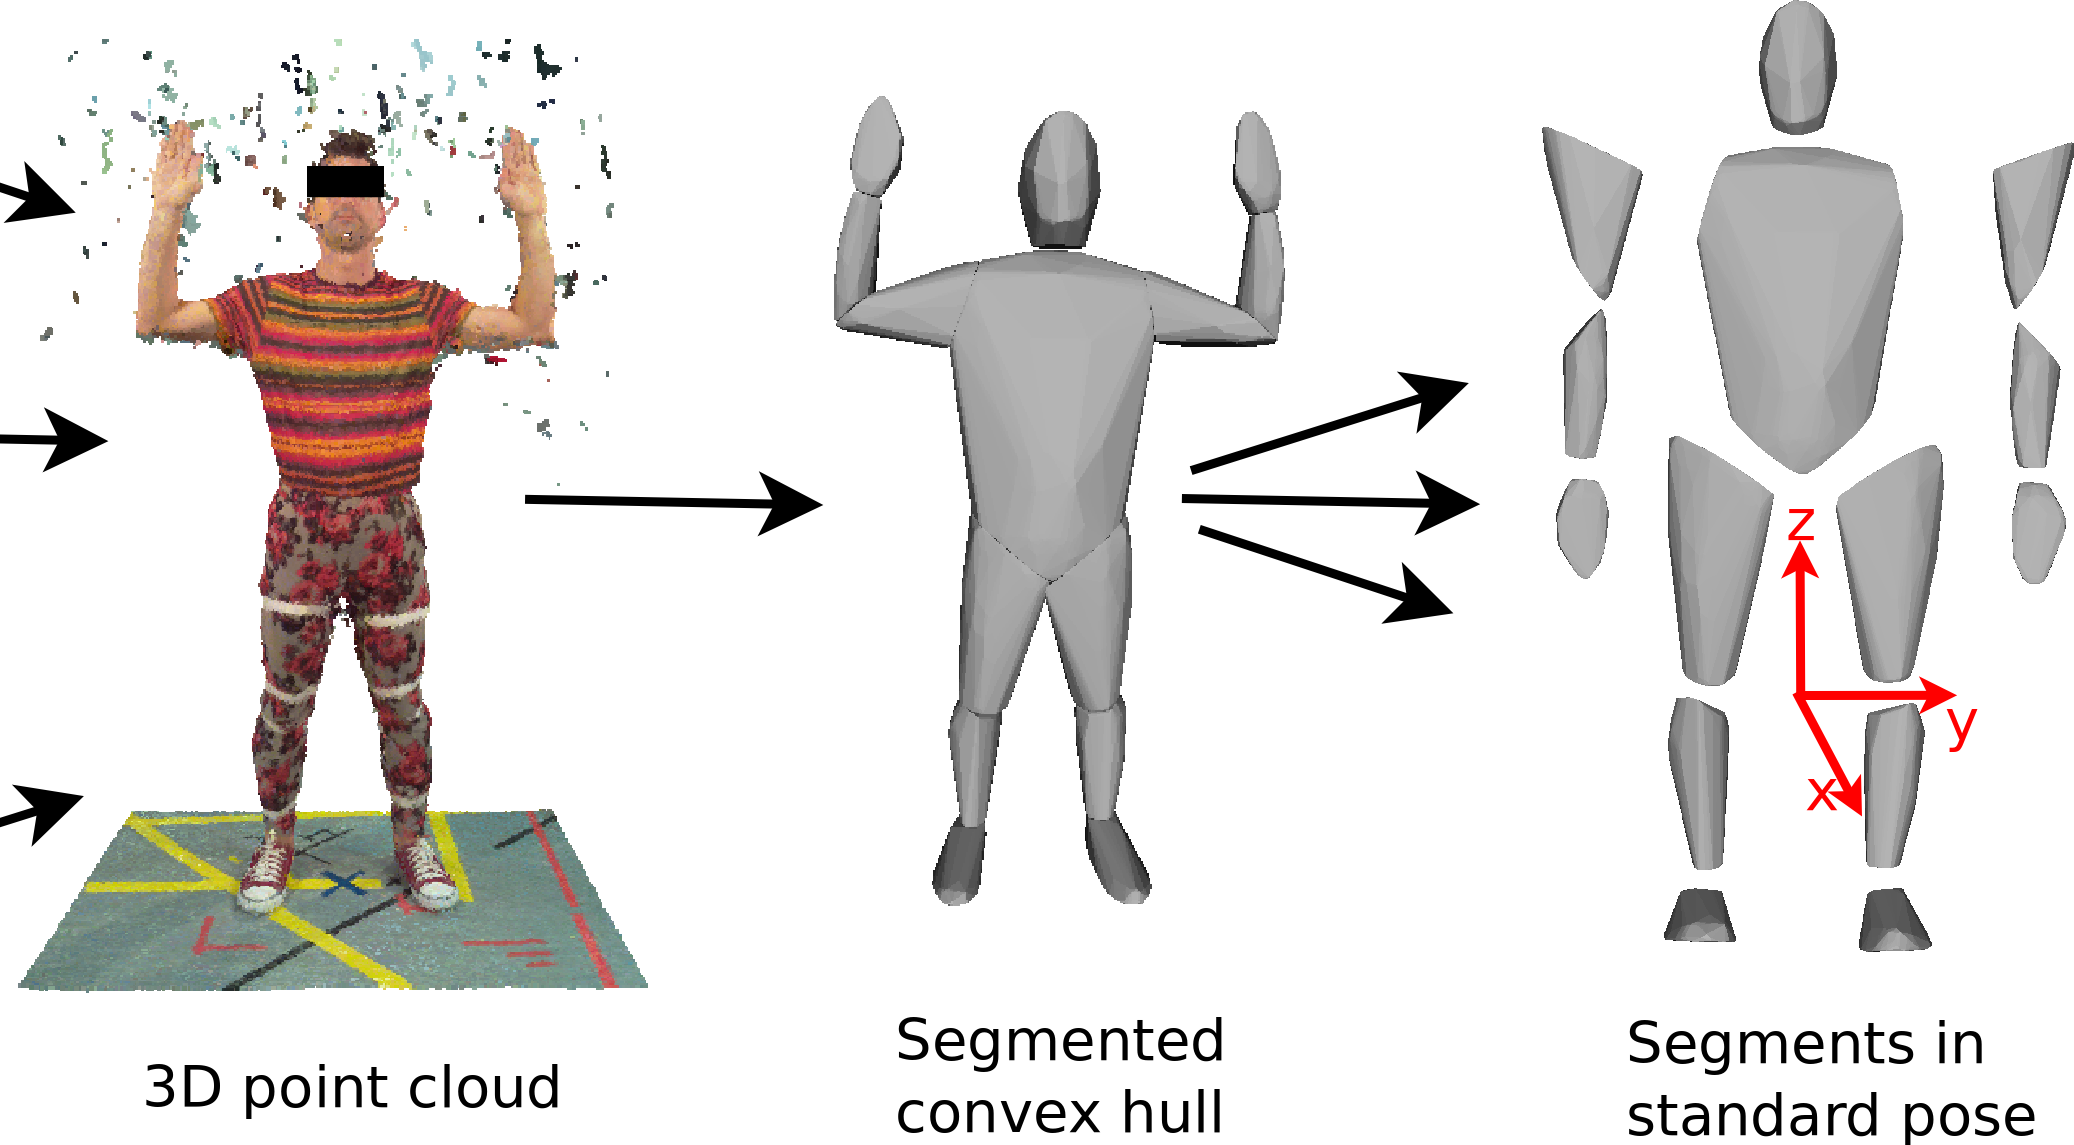
\includegraphics[width=0.7\linewidth]{reconstructionWorkflow}
	\caption{General approach to estimate the pose of a real object, including 3D scanning and reconstruction, 3D segmentation to get the joints and subsequently skeleton extraction}
	\label{fig:posecapture}
\end{figure}
%
\subsection{3D Scanning/Reconstruction}
\label{sec:reconstruction}
%
% ToDo: explain in detail
%
Scanning means collecting a real shape as 3D data. Reconstruction means the approach to convert the raw data to a mesh or process the input data.

Voxelization, Shape from Shilouette, Shape from Shading, Depth camera, stereo camera
%
%TODO: add all references (shape fitting, ...)
%
\subsection{3D Segmentation}
\label{sec:segmentation}
%
% ToDo: explain methods in detail
% 1) markers/sensors/exoskeleton
% 2) markerless methods
%
How it is done: markers, sensors, shape fitting (already known)
Cite all papers (Voxelization, ....). There are previous approaches with markers and sensors which will not be treated in this work in detail, as markerless options are taken as focus.

\subsubsection{Supervised methods}
Many already existing methods don't require markers and sensors but already assume or know the hierarchical structure or the body parts of the object to be captured (see \cite{multiLayerSkeleton}, \cite{baker2005shape}, \cite{de2008hierarchical} and \cite{michoud2007real}).

\subsubsection{Unsupervised methods}
Although the approaches mentioned in section \ref{sec:currentApproaches} work quite well depending on the application, improvements can be made that are more independent from user inputs.... which leads us to the non-rigid registration \ref{nonrigidregistration}.

\section{Non-rigid registration}
\label{nonrigidregistration}

Generally, registration means the alignment of rigid point clouds (see figure \ref{fig:registration}). A well-known approach to achieve this, is the iterative closest point (ICP) \cite{ICP}, which requires the input point clouds to be aligned quite similar to avoid a local optimum. After registration, a matching error $e$ is achieved, which states the total euclidean distance between the associated points of the registered point clouds. In case of two non-rigid objects (e.g. a human in different poses which is composed of rigid parts) the ICP won't lead to a satisfying registration as associated parts are transformed differently. In order to register a non-rigid object, a segmentation into its rigid parts is required.

\subsection{Challenges}
\label{Challenges}
There are many challenges regarding the non-rigid registration of point clouds in 2D, as well as in 3D. First off, the input data can be noisy by means of points not belonging to the object. Furthermore, the approach is computationally expensive and time-consuming, as the corresponding body parts of two meshes need to be detected iteratively. Additionally, the inevitable difficulty of finding the global optimum, related to ambiguous body parts, has to be overcome.

\begin{figure}[H]
	\centering\small
	\begin{tabular}{cc}
		\fbox{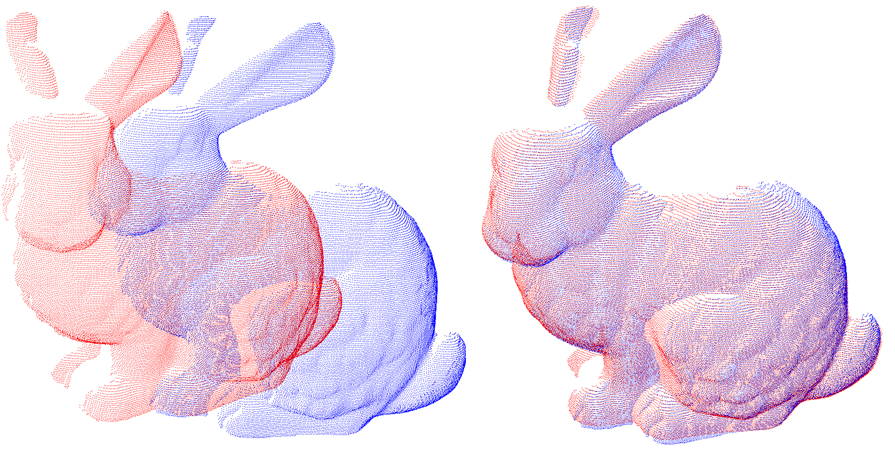
\includegraphics[width=0.43\textwidth]{stanfordBunny}} &		% JPEG file
		\fbox{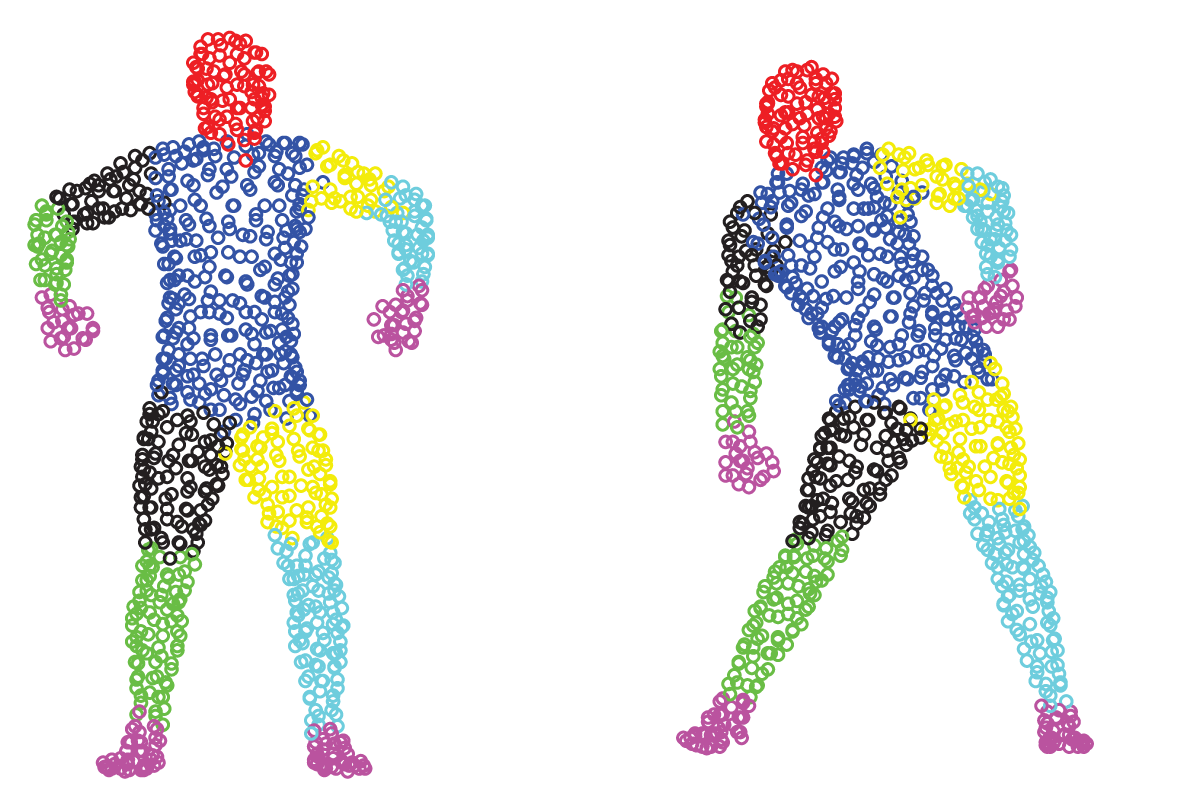
\includegraphics[width=0.45\textwidth]{nonrigidregistration}} 
		\\	% PNG file
		(a) & (b) 
	\end{tabular}
	\caption{Rigid registration of the stanford bunny~(a) \cite{stanfordBunny} and non-rigid registration of a human~(b) \cite{registrationHuman} by detecting its rigid parts.}
	
	\label{fig:registration}
\end{figure}\textbf{}

\section{Related work}
\label{sec:RelatedWork}

By focusing on approaches computing the segmentation of articulated objects from 3D data, many different ones could be detected. They face similar challenges (see subsection \ref{Challenges}) but solve them in different ways
%%
\subsection{Correlated Correspondence}

A main approach for non-rigid registration is proposed by Anguelov \cite{Anguelov04} applying the correlated correspondence algorithm \cite{CorrelatedCorrespondance}. The algorithm takes a \textit{template} Mesh $D_0$ and other Meshes $D_1,\ldots,D_n$ in different configurations as input. The algorithm then performs a probabilistic framework and Expectation-Maximization (EM) to iterate between finding a decomposition of the \textit{template} into rigid parts and detecting them in the other meshes. Furthermore, a random clustering is applied to facilitate the detection of associated rigid parts.
%%
\begin{figure}
	\centering
	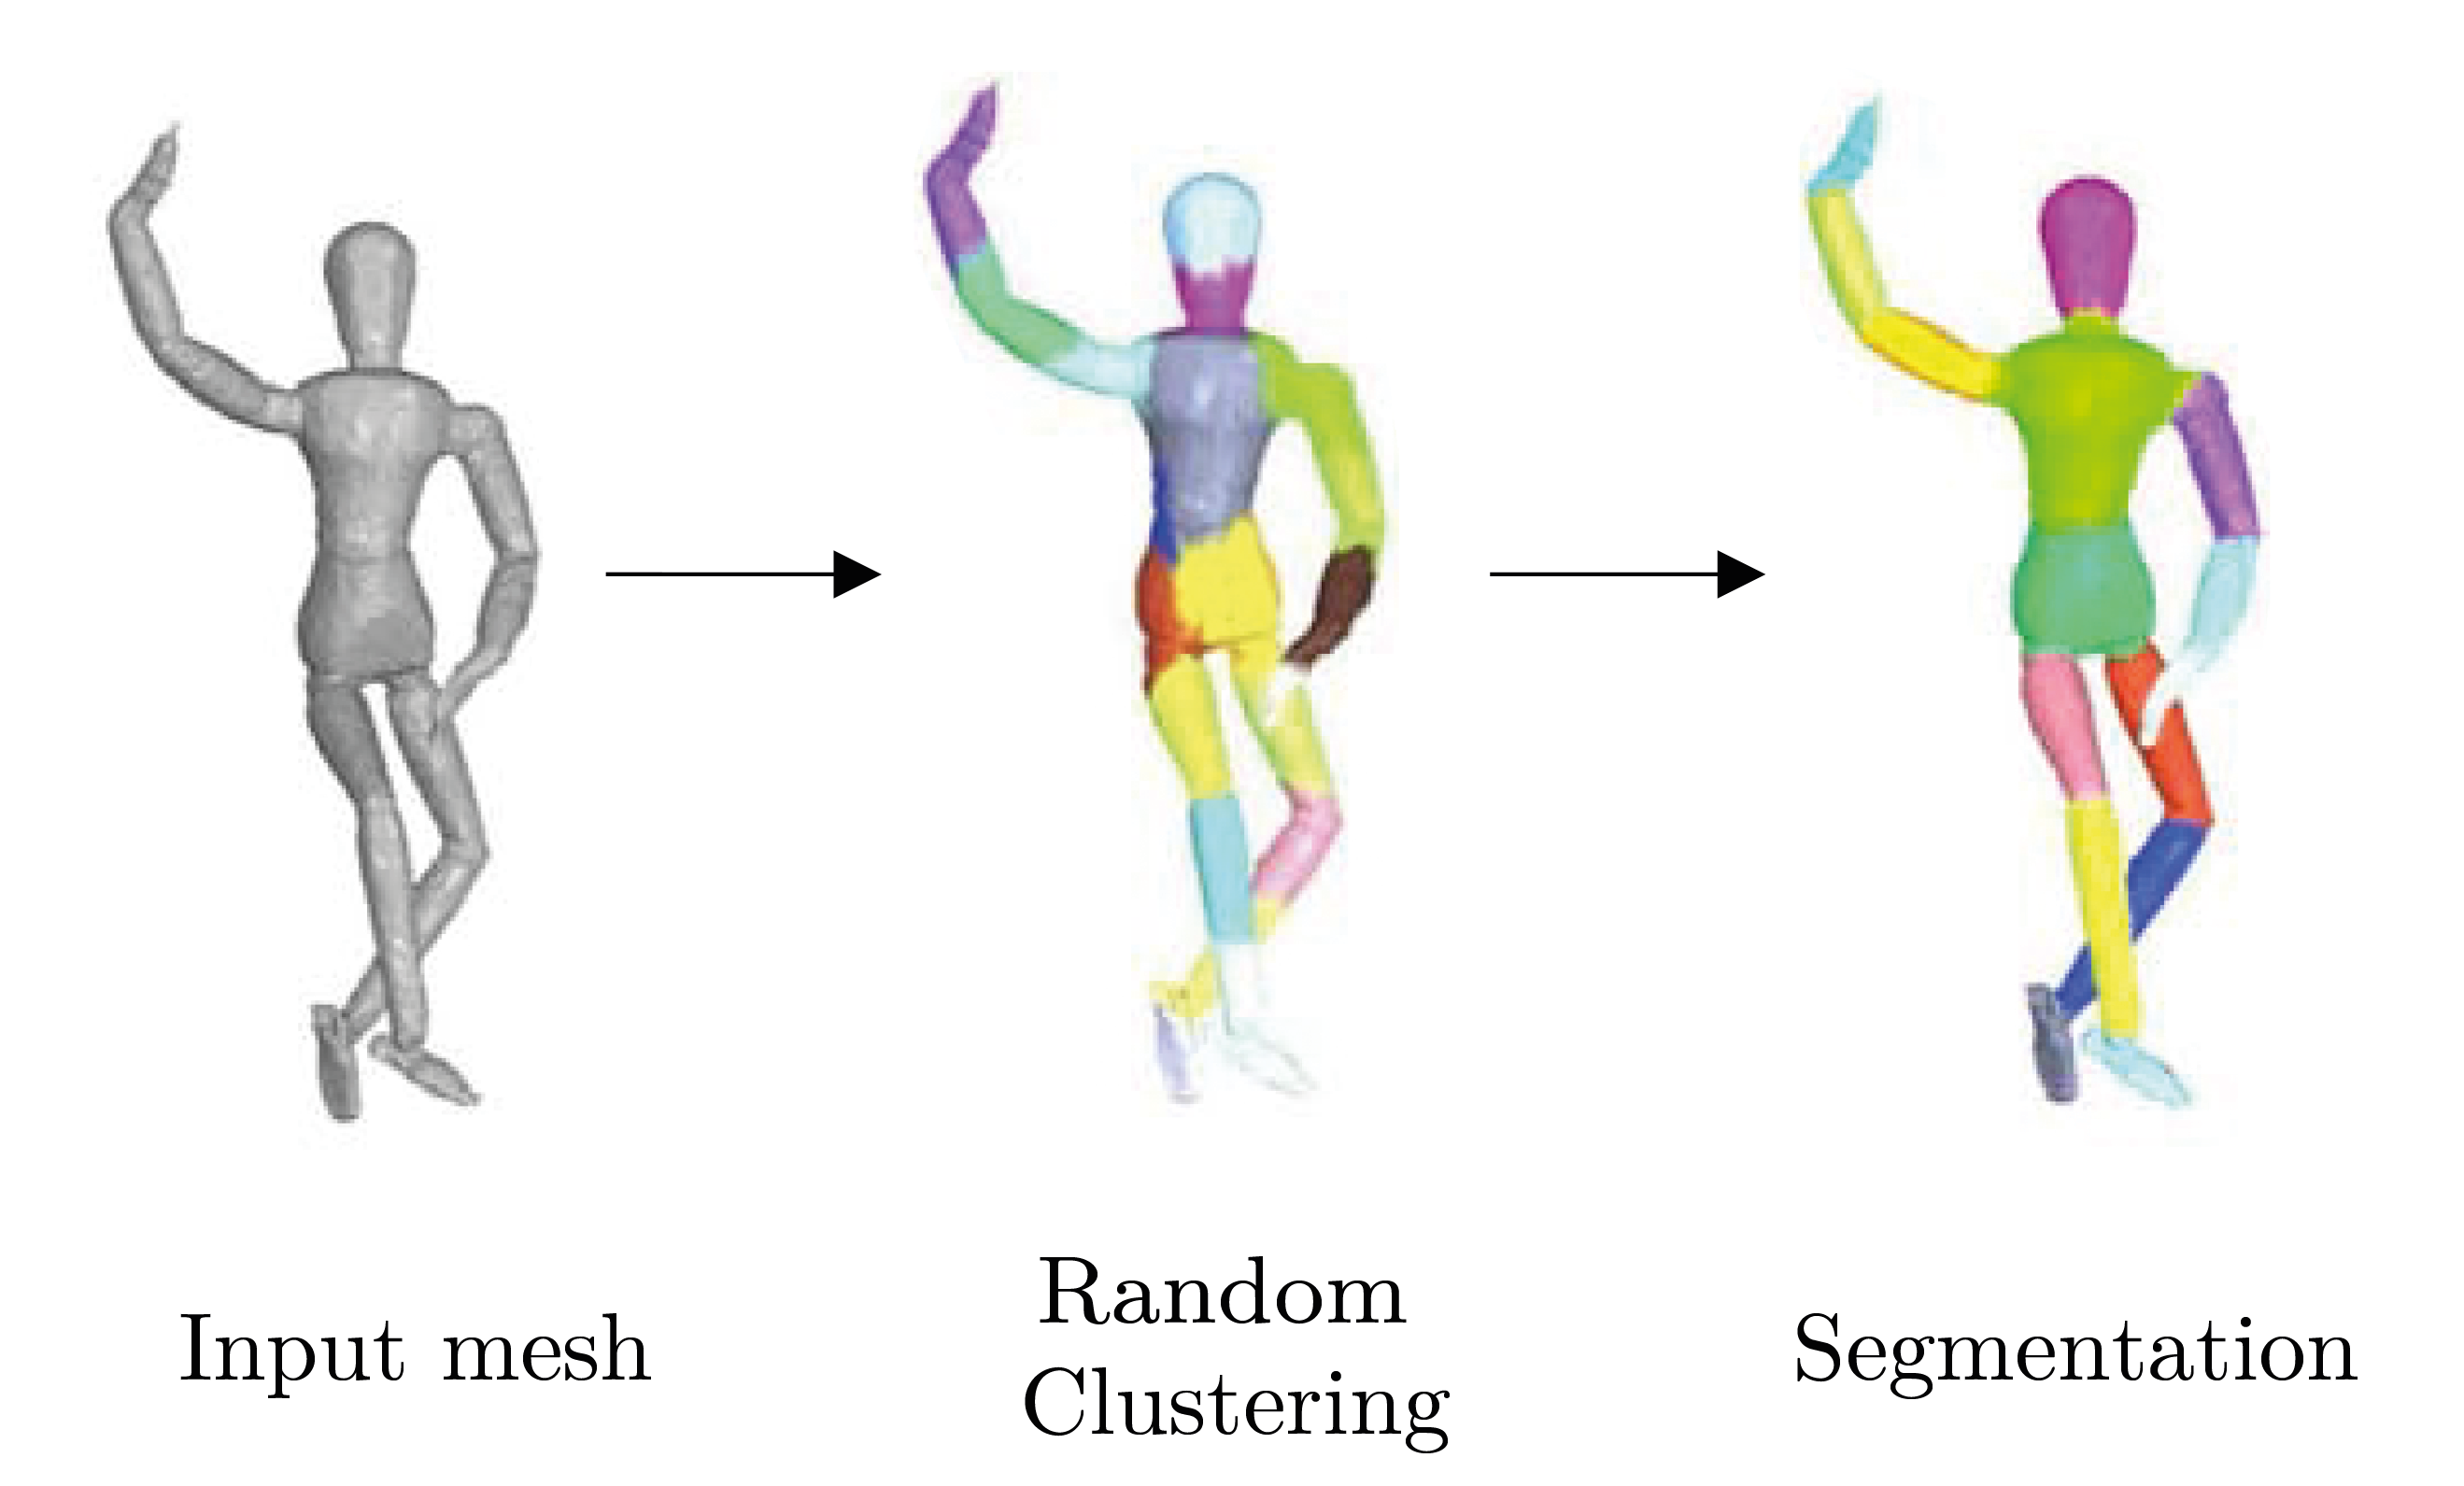
\includegraphics[width=0.7\linewidth]{anguelov}
	\caption{Segmentation a template mesh $M$ into its rigid parts by applying random clustering and a probabilistic framework to iteratively detect associating parts in another mesh \cite{Anguelov04}.}
	\label{fig:correlatedcorrespondance}
\end{figure}
%%
A different approach proposes the recursive detection of body parts by the LRP -- ``largest rigid part'' algorithm \cite {guo2016correspondence}. 
%%
\subsection{LRP}
The LRP algorithm discovers the articulated parts of two objects in different configurations by initially detecting the largest rigid part. This would be the biggest point cluster by applying a single rigid transformation. To reach that, sparse correspondences in combination with RANSAC are implemented. From there, the linking parts are recursively detected by growing clusters from the LRP and reapplying the algorithm. 
%%
\begin{figure}[H]
	\centering\small
	\begin{tabular}{cc}
		\fbox{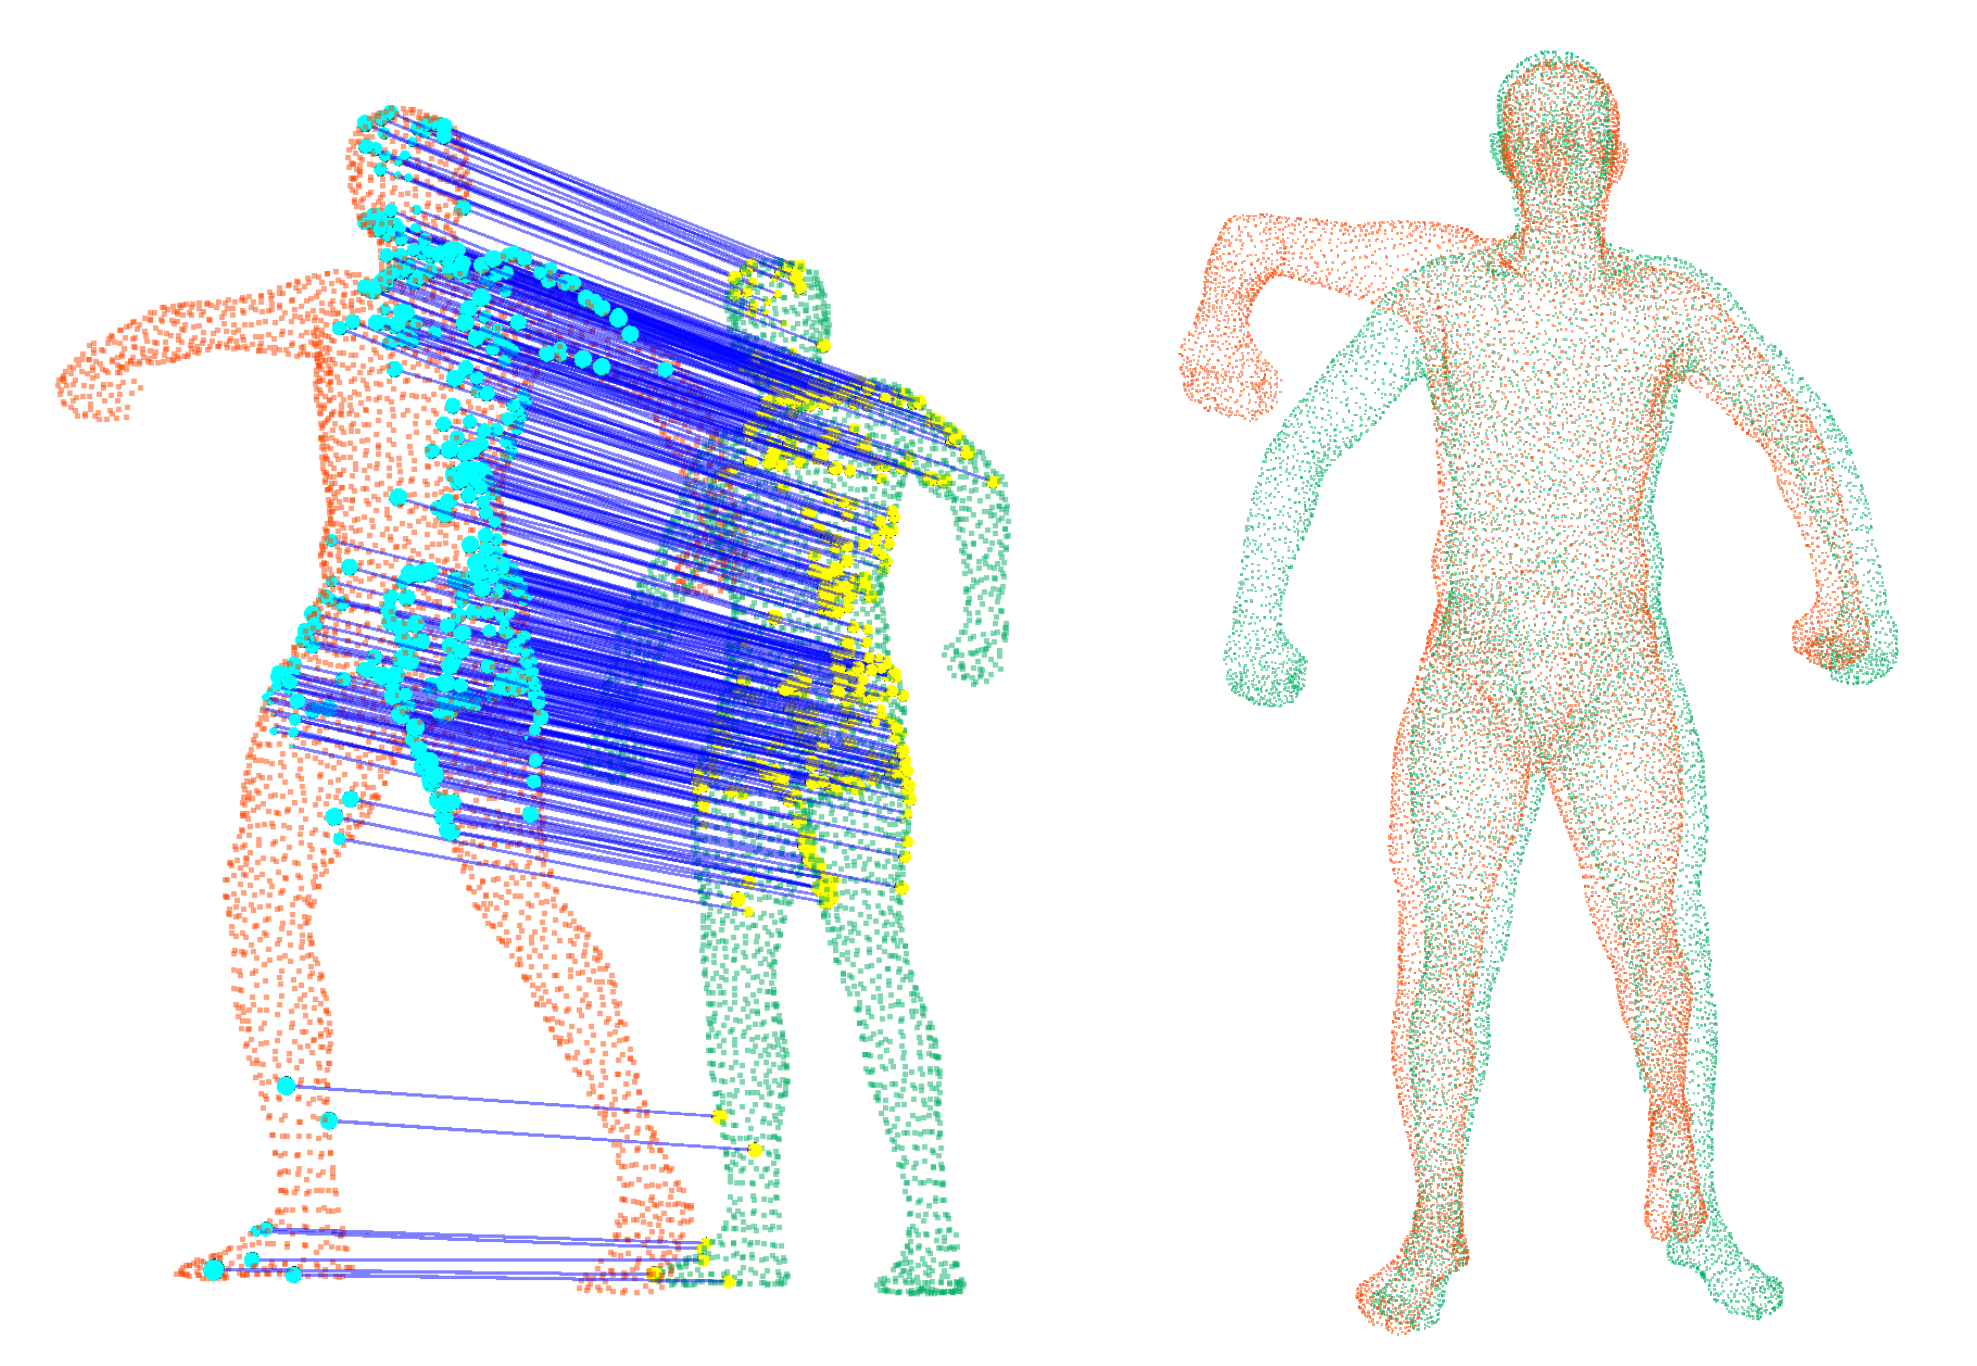
\includegraphics[width=0.45\textwidth]{LRP_body}} &	
		\fbox{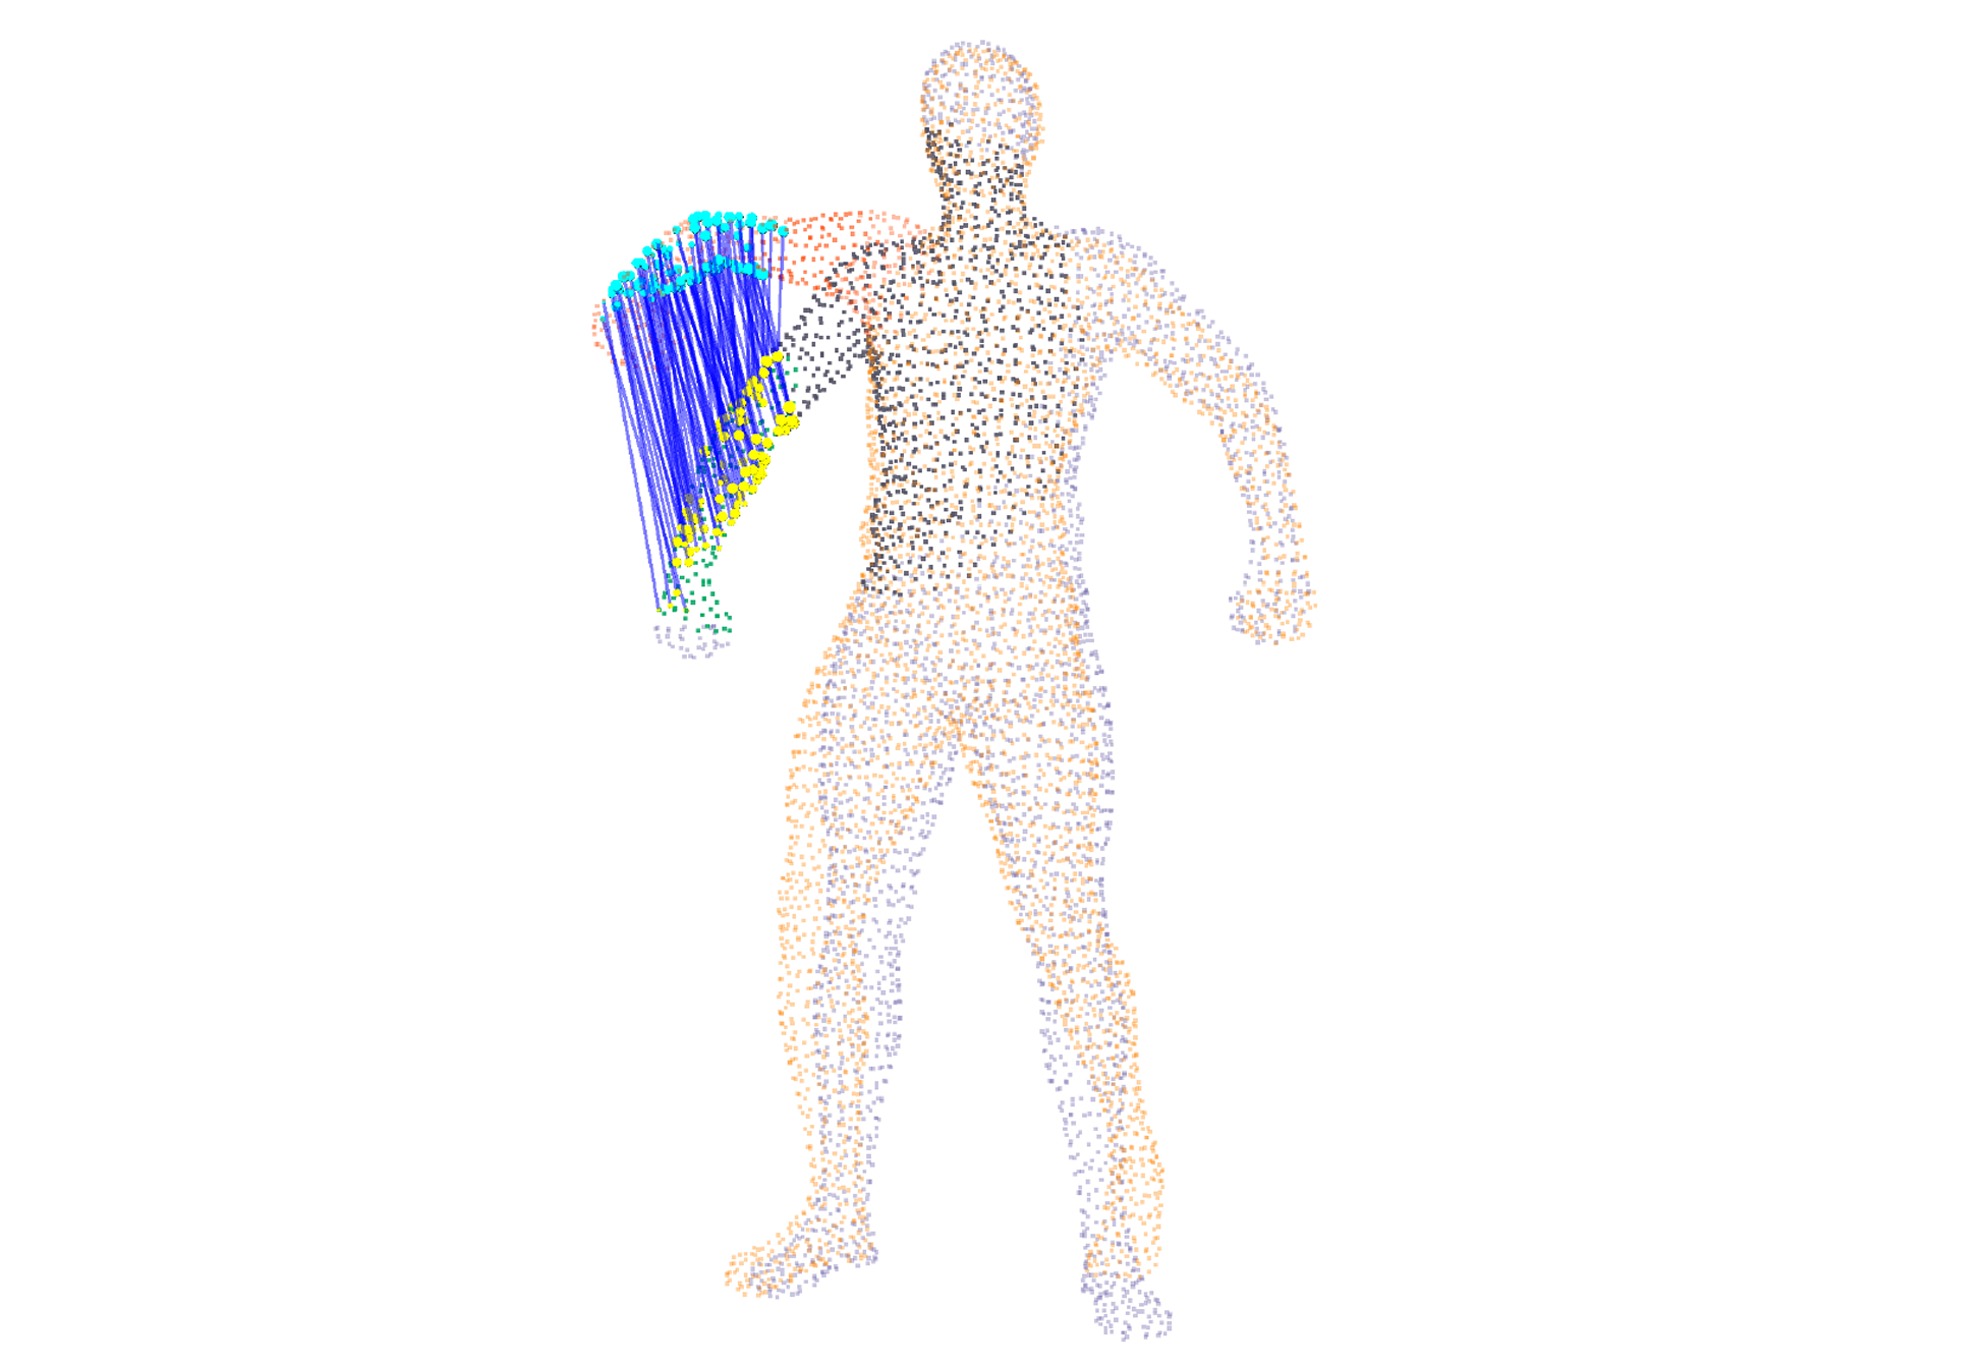
\includegraphics[width=0.45\textwidth]{LRP_arm}} 
		\\
		(a) & (b) 
	\end{tabular}
	\caption{Detecting the largest rigid part of an object~(a), and align the object to recursively detect linking parts to the LRP~(b) \cite{guo2016correspondence}.} 
	\label{fig:LRP_algorithm}
\end{figure}
%%
Another approach is achieved by Symmetrization \cite{Mitra07}, by detecting and aligning the body parts’ symmetry axes of an object(see figure \ref{fig:Symmetrization}). Based on Anguelov \cite{Anguelov04} and Mitra \cite{Mitra07}, Chang et al developed a closely related approach \cite{chang08articulated} \cite{chang09range}.
%%
\begin{figure}[H]
	\centering\small
	\begin{tabular}{cc}
		\fbox{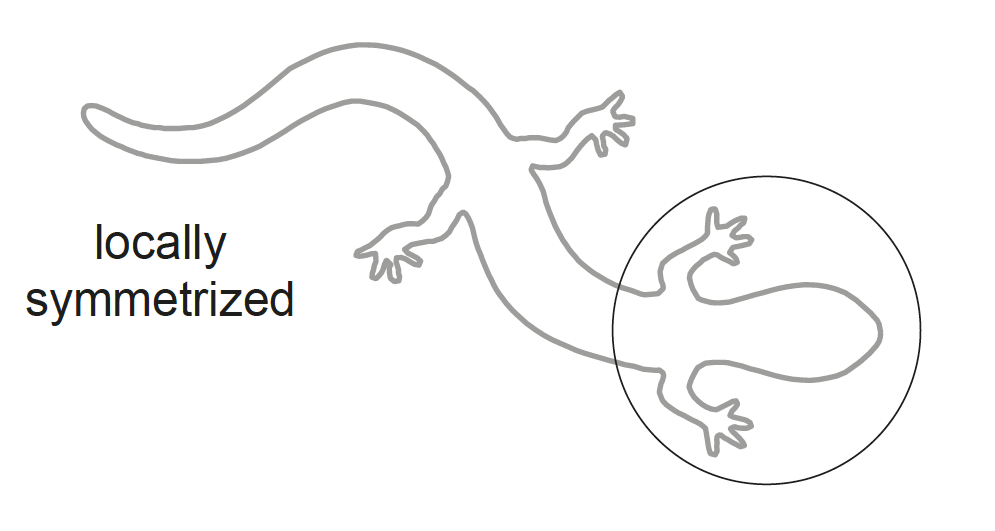
\includegraphics[width=0.45\textwidth]{Symmetrization1}} &
		\fbox{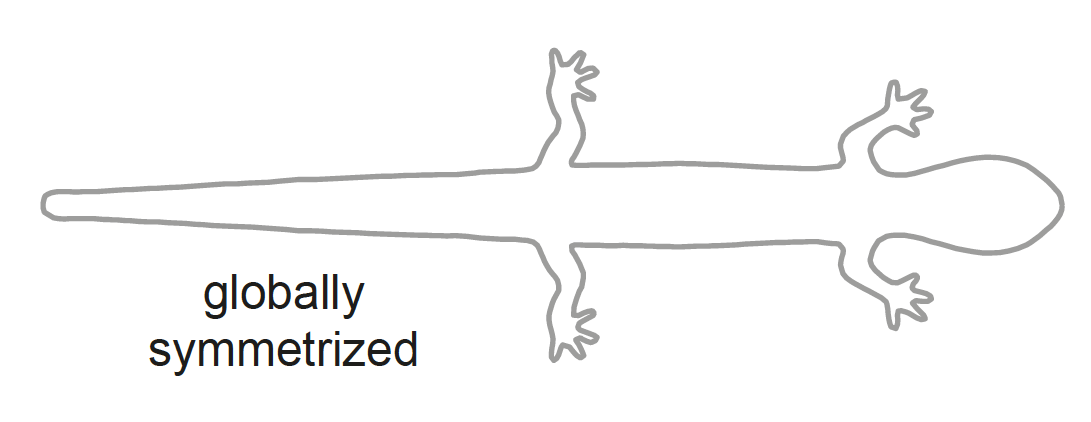
\includegraphics[width=0.45\textwidth]{Symmetrization2}} 
		\\
		(a) & (b) 
	\end{tabular}
	\caption{Detection of the rigid parts of an object by local~(a) and global~(b) Symmetrization \cite{Mitra07}.} 
	\label{fig:Symmetrization}
\end{figure}
%%

%TODO: Add other references
\subsection{Possible improvements}

%TODO: What are the main deficits of the algorithms?

The proposed approaches achieve convincing results concerning the accuracy of the segmentation and the detection of rigid parts. However, they are all computationally expensive and require a considerable number of computation steps to iteratively detect rigid parts in two associated objects. This reflects on the run time of the algorithm which offers therefore great potential for improvements.

Taking the existing methods as reference (see chapter \ref{cha:RelatedWork}) a new segmentation approach is developed. Thereby, the main focus is to reduce the computation steps of the correlated correspondence algorithm \cite{CorrelatedCorrespondance} as well as the LRP algorithm \cite {guo2016correspondence}. To fully focus on the segmentation into its rigid part, the 3D reconstruction of the articulated object is assumed to be available.
%\chapter{Related work}
\label{cha:RelatedWork}

By focusing on approaches computing the segmentation of articulated objects from 3D data, many different ones could be detected. They face similar challenges (see subsection \ref{Challenges}) but solve them in different ways
%%
\section{Correlated Correspondence}

A main approach for non-rigid registration is proposed by Anguelov \cite{Anguelov04} applying the correlated correspondence algorithm \cite{CorrelatedCorrespondance}. The algorithm takes a \textit{template} Mesh $D_0$ and other Meshes $D_1,\ldots,D_n$ in different configurations as input. The algorithm then performs a probabilistic framework and Expectation-Maximization (EM) to iterate between finding a decomposition of the \textit{template} into rigid parts and detecting them in the other meshes. Furthermore, a random clustering is applied to facilitate the detection of associated rigid parts.
%%
\begin{figure}
	\centering
	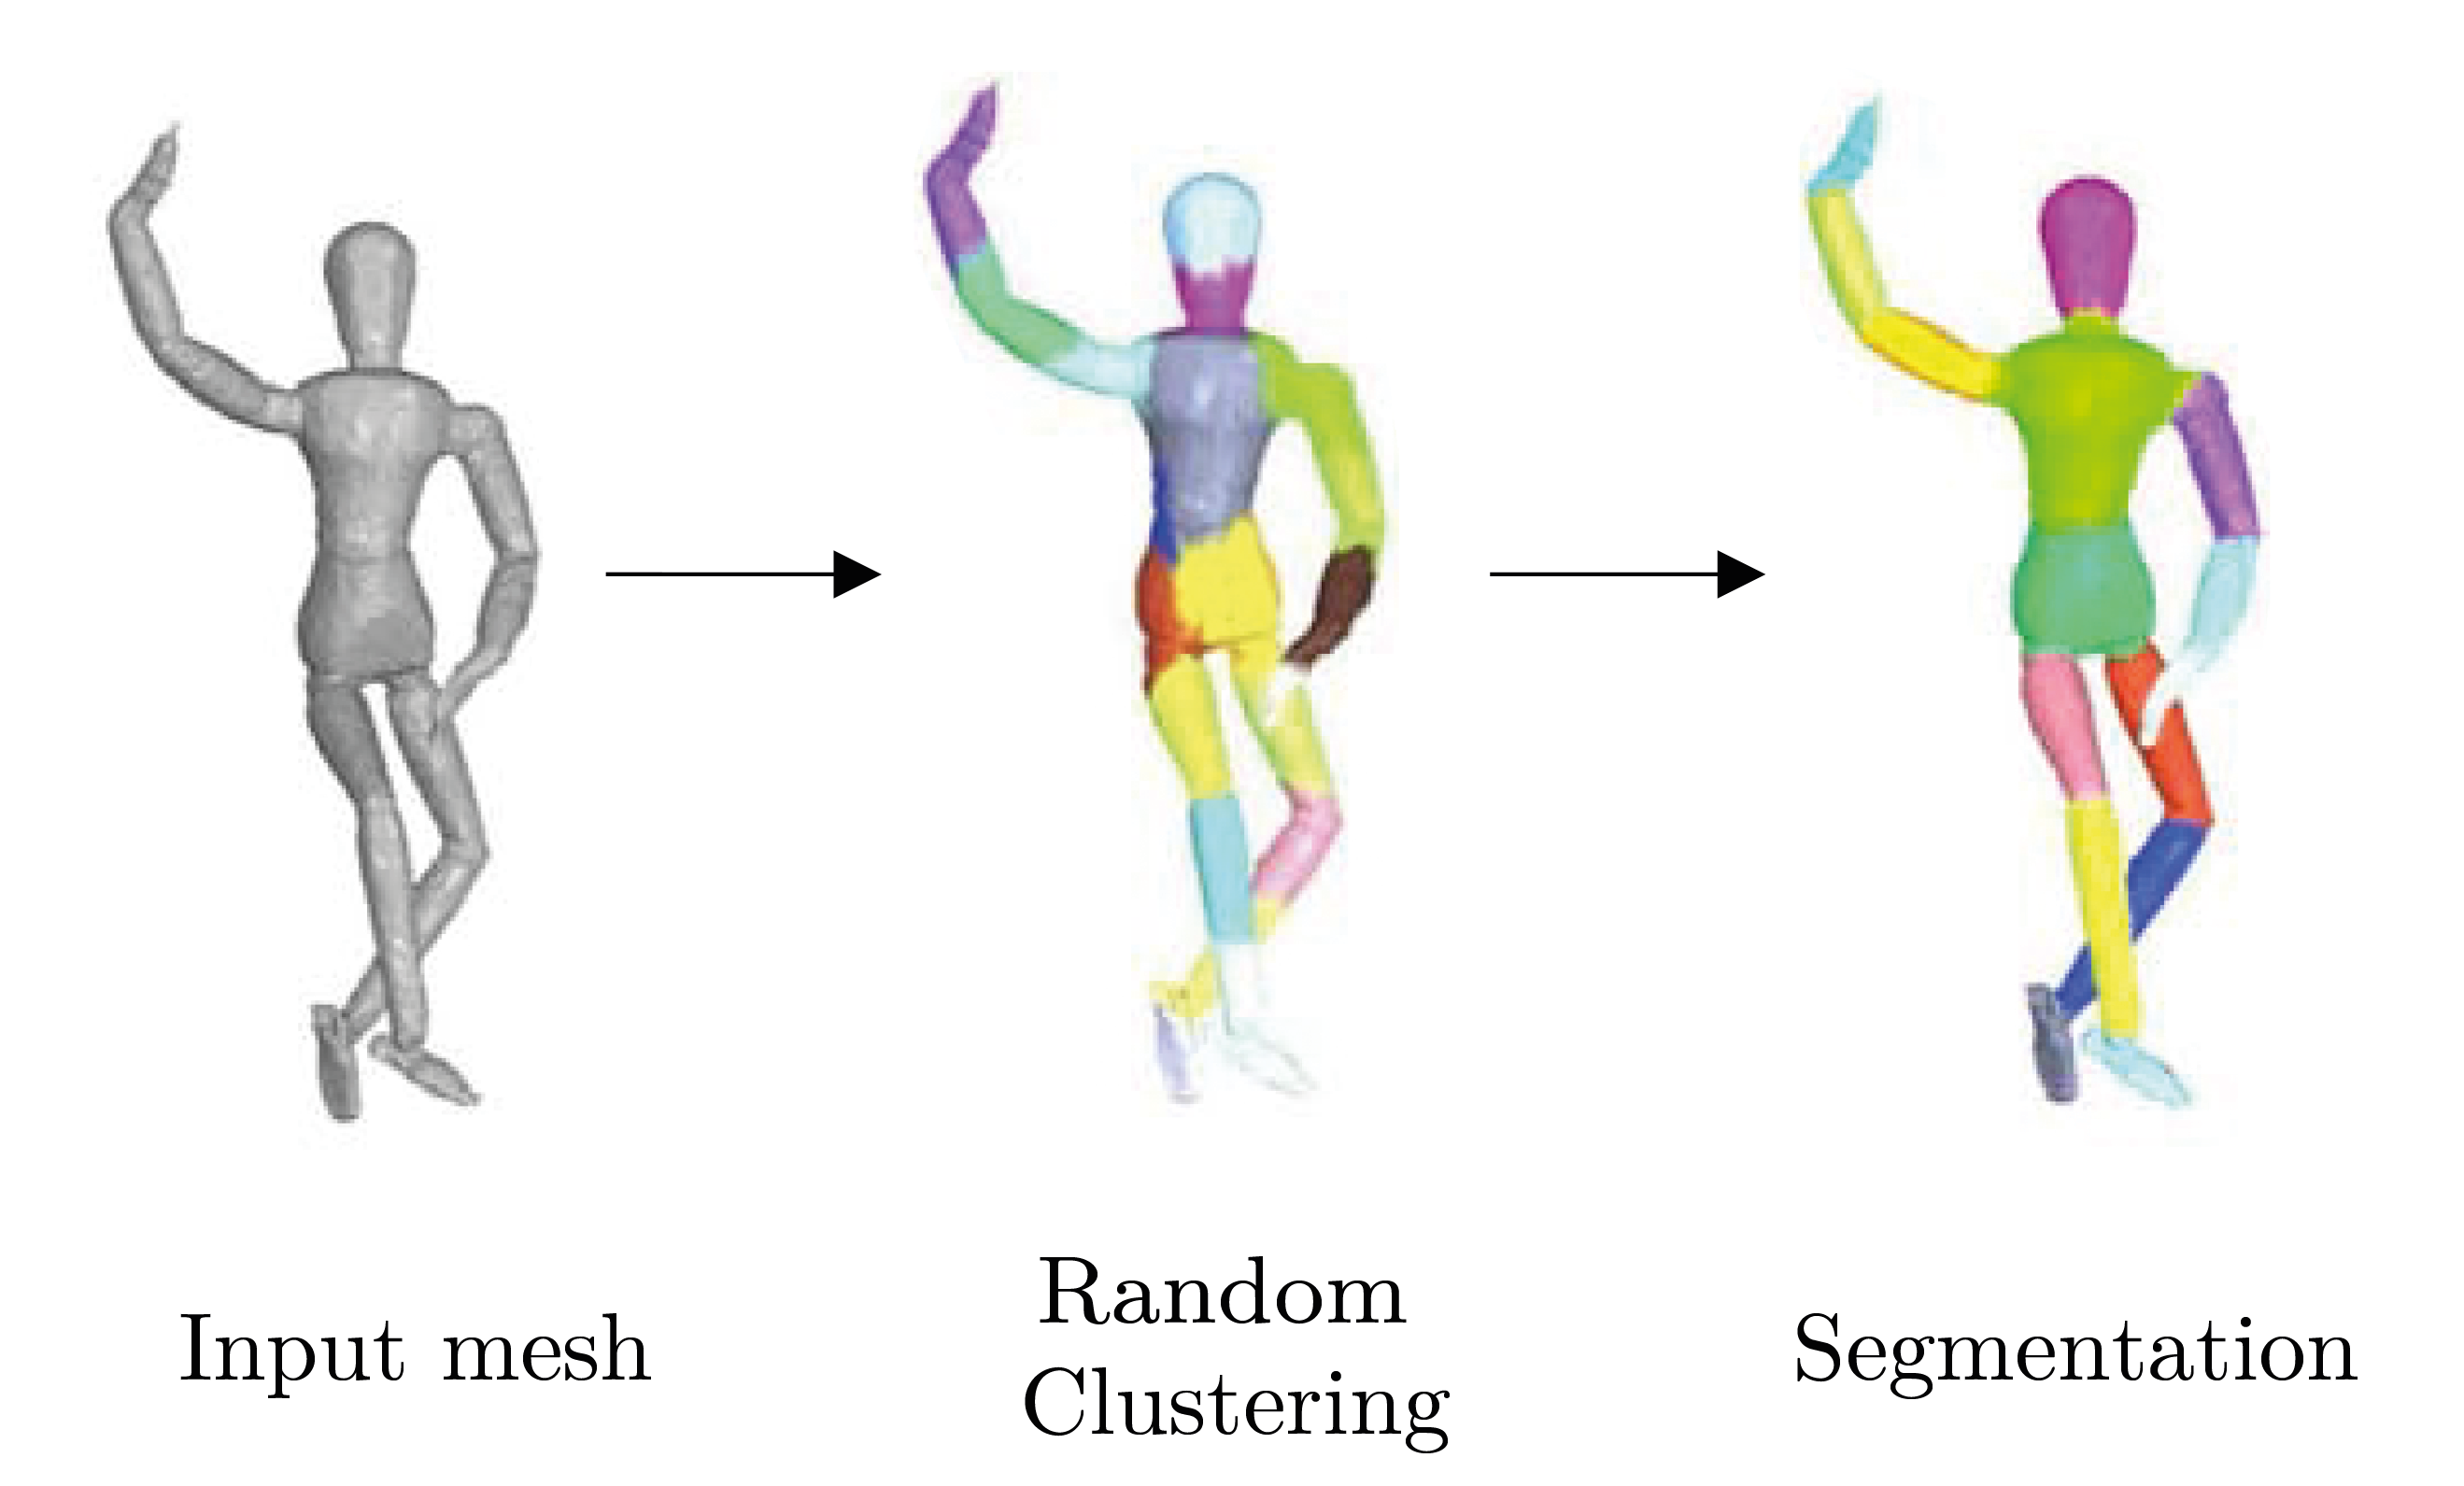
\includegraphics[width=0.7\linewidth]{anguelov}
	\caption{Segmentation a template mesh $M$ into its rigid parts by applying random clustering and a probabilistic framework to iteratively detect associating parts in another mesh \cite{Anguelov04}.}
	\label{fig:correlatedcorrespondance}
\end{figure}
%%
A different approach proposes the recursive detection of body parts by the LRP -- ``largest rigid part'' algorithm \cite {guo2016correspondence}. 
%%
\section{LRP}
The LRP algorithm discovers the articulated parts of two objects in different configurations by initially detecting the largest rigid part. This would be the biggest point cluster by applying a single rigid transformation. To reach that, sparse correspondences in combination with RANSAC are implemented. From there, the linking parts are recursively detected by growing clusters from the LRP and reapplying the algorithm. 
%%
\begin{figure}[H]
	\centering\small
	\begin{tabular}{cc}
		\fbox{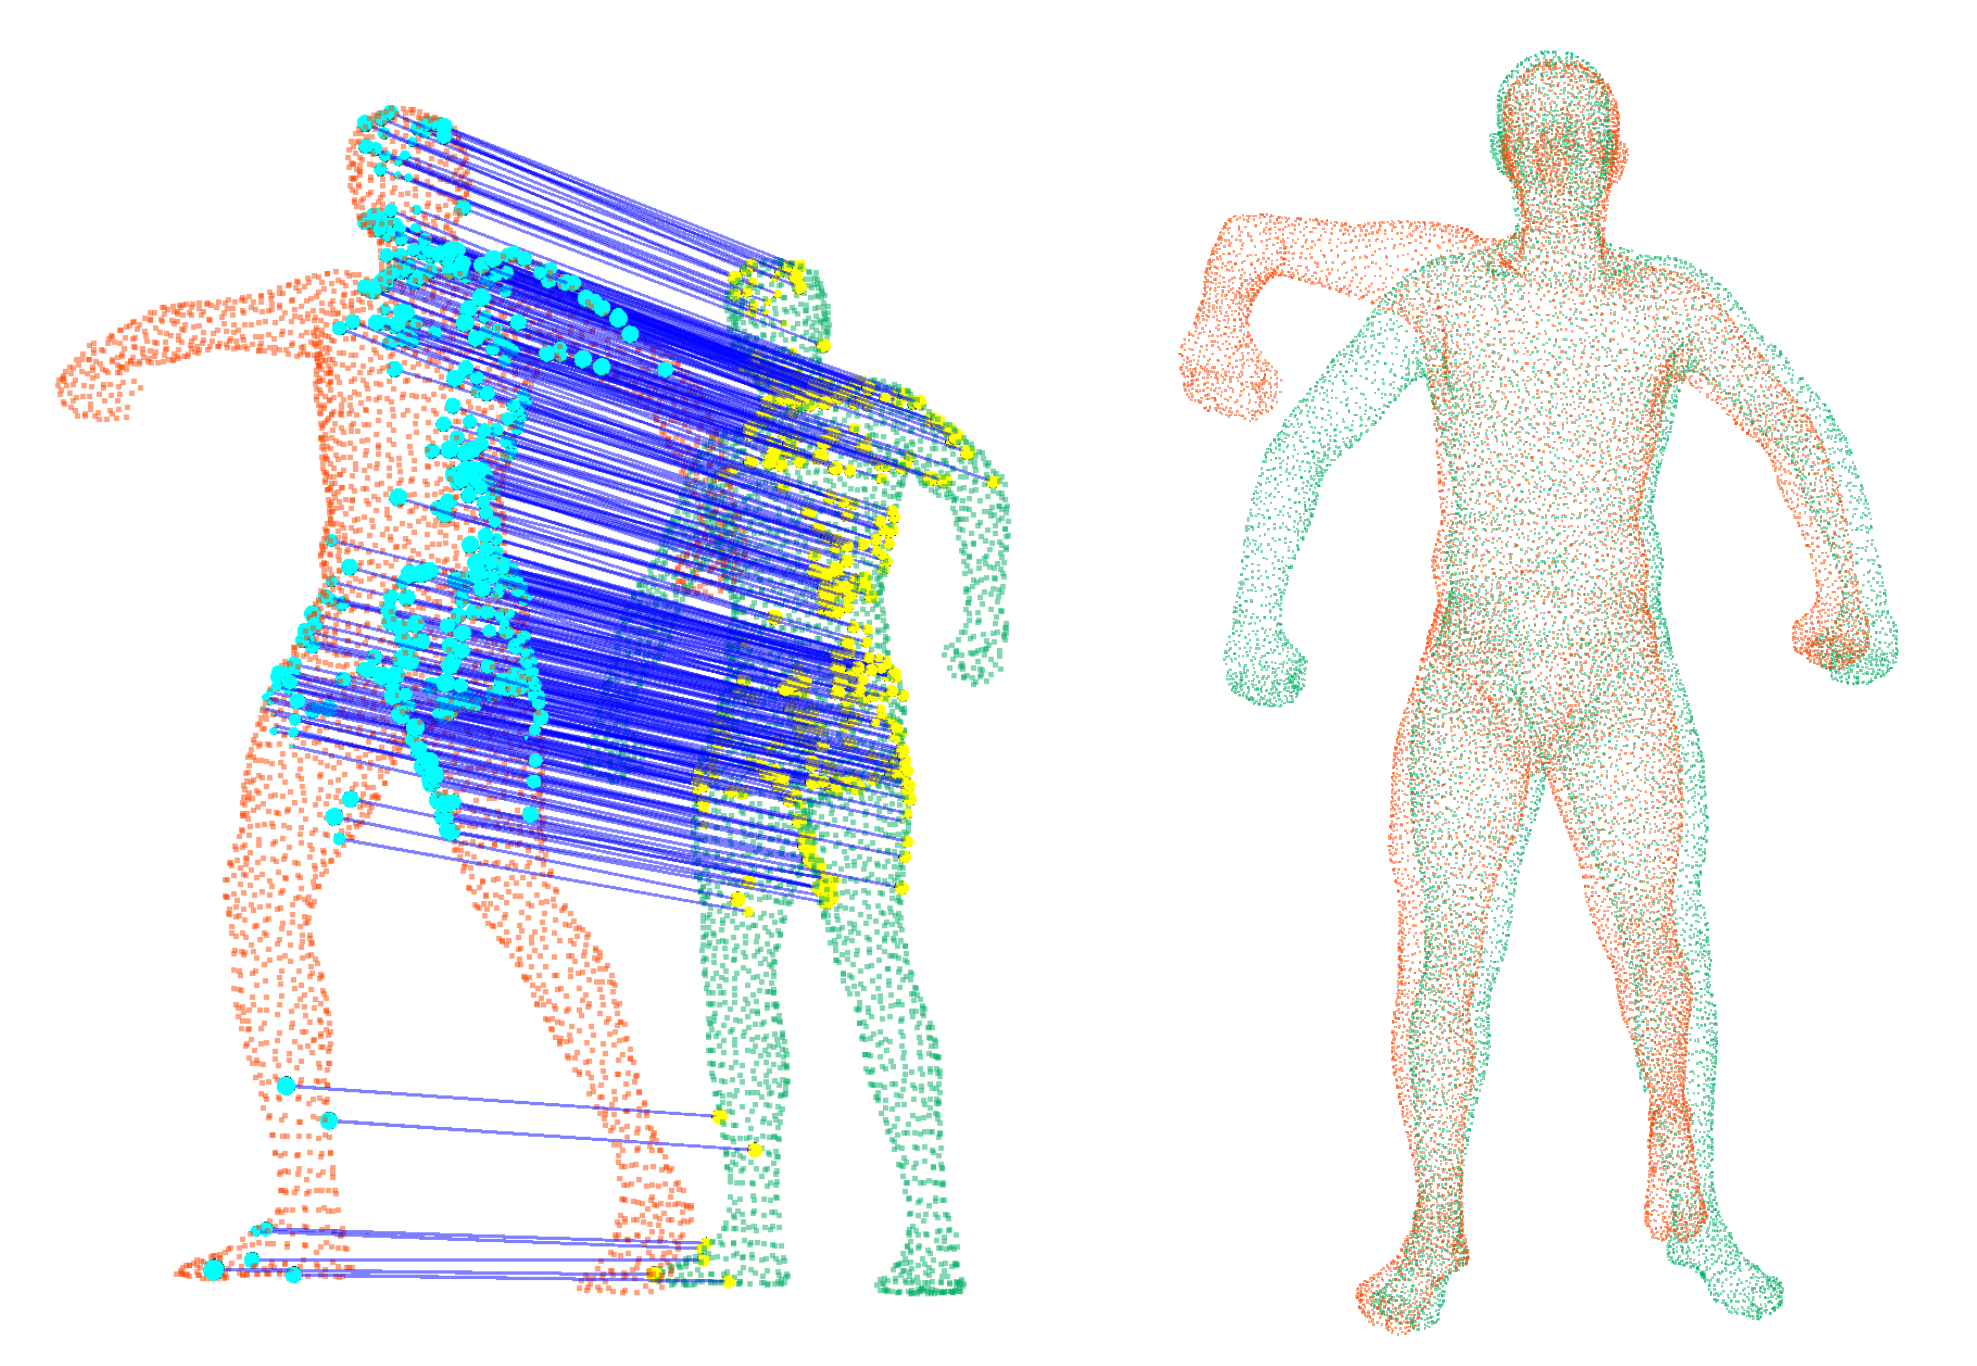
\includegraphics[width=0.45\textwidth]{LRP_body}} &	
		\fbox{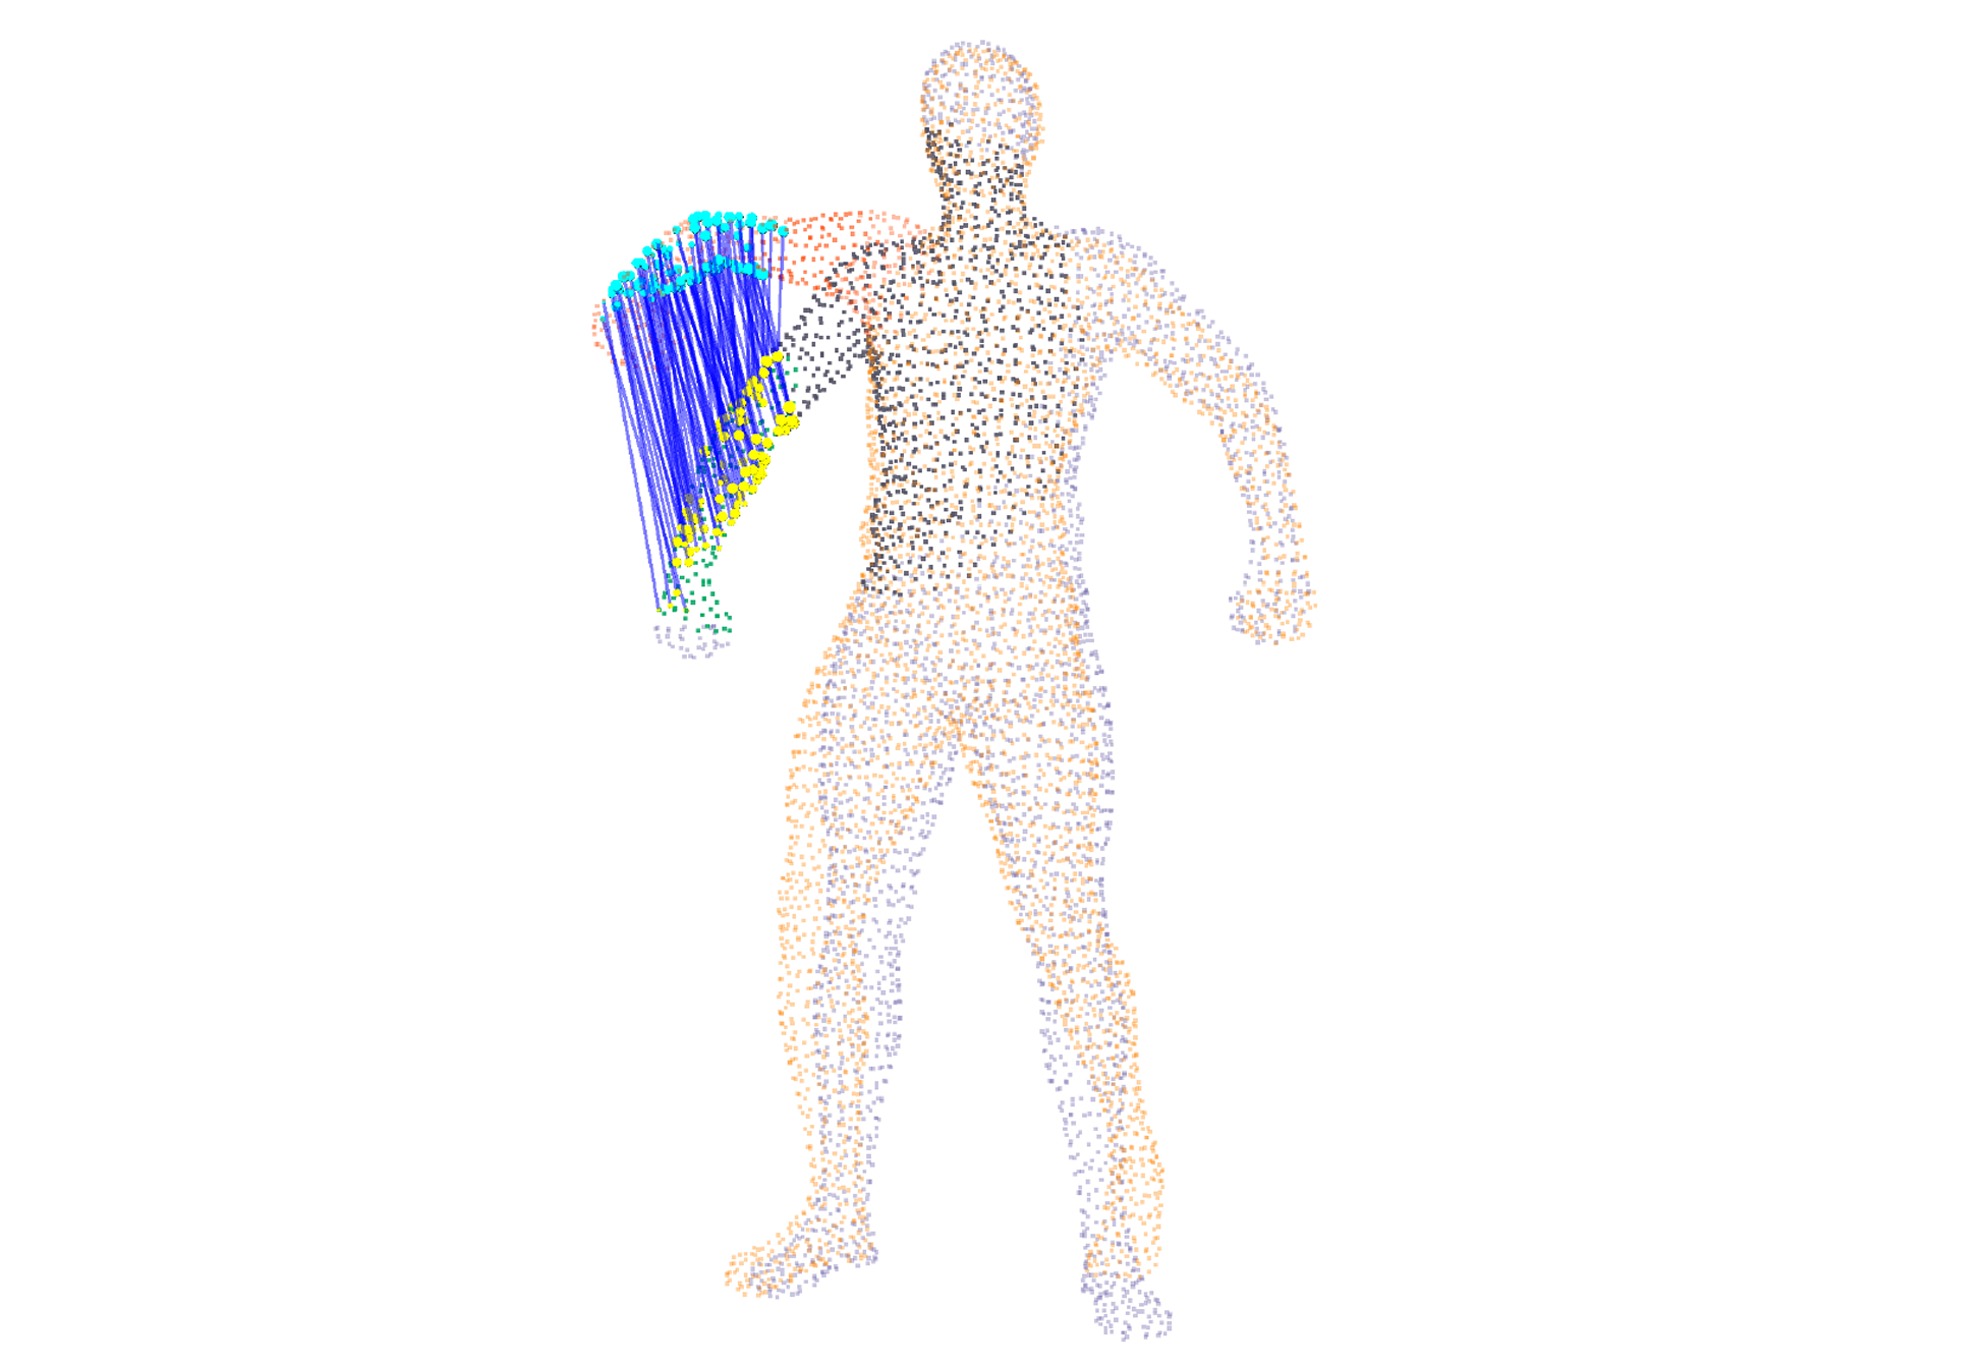
\includegraphics[width=0.45\textwidth]{LRP_arm}} 
		\\
		(a) & (b) 
	\end{tabular}
	\caption{Detecting the largest rigid part of an object~(a), and align the object to recursively detect linking parts to the LRP~(b) \cite{guo2016correspondence}.} 
	\label{fig:LRP_algorithm}
\end{figure}
%%
Another approach is achieved by Symmetrization \cite{Mitra07}, by detecting and aligning the body parts’ symmetry axes of an object(see figure \ref{fig:Symmetrization}). Based on Anguelov \cite{Anguelov04} and Mitra \cite{Mitra07}, Chang et al developed a closely related approach \cite{chang08articulated} \cite{chang09range}.
%%
\begin{figure}[H]
	\centering\small
	\begin{tabular}{cc}
		\fbox{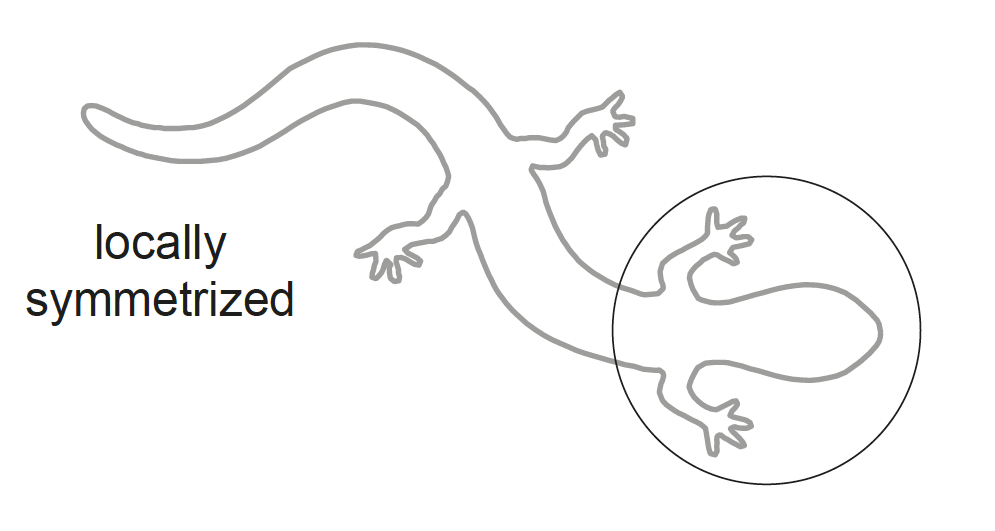
\includegraphics[width=0.45\textwidth]{Symmetrization1}} &
		\fbox{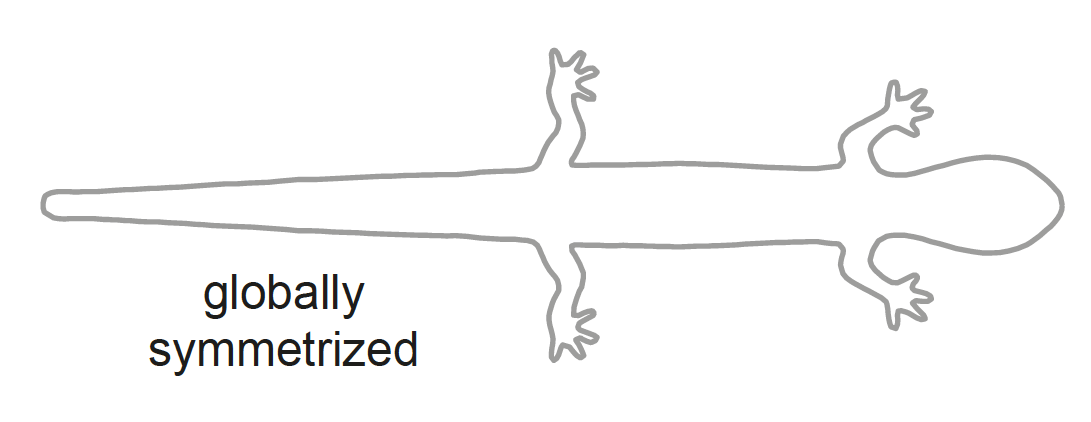
\includegraphics[width=0.45\textwidth]{Symmetrization2}} 
		\\
		(a) & (b) 
	\end{tabular}
	\caption{Detection of the rigid parts of an object by local~(a) and global~(b) Symmetrization \cite{Mitra07}.} 
	\label{fig:Symmetrization}
\end{figure}
%%

%TODO: Add other references
\section{Possible improvements}

%TODO: What are the main deficits of the algorithms?

The proposed approaches achieve convincing results concerning the accuracy of the segmentation and the detection of rigid parts. However, they are all computationally expensive and require a considerable number of computation steps to iteratively detect rigid parts in two associated objects. This reflects on the run time of the algorithm which offers therefore great potential for improvements. %% added to introduction
\chapter{Notation}
\label{cha:Notation}

\begin{itemize}
	%use \dotfill for points
	\item[$M$] Input mesh
	\item[$\mathcal{P}$] set of rigid parts
	\item[$\mathcal{J}$] set of joints
	\item[$\mathcal{C}$] set of clusters
	\item[$\mathcal{T}$] set of transformations
	\item[$C_i$] cluster
	\item[$C_{i,j,\cdots}$] sub cluster with varying depth
	\item[$p_i$] principal axis of $C_i$
	\item[$s_i$] secondary axis of $C_i$
	\item[$\theta$] orientation of $C_i$
	\item[$\boldsymbol{p}_i(x,y)$] 2D cluster point of $C_i$
	\item[$\boldsymbol{p}_i(x,y,z)$] 3D cluster point of $C_i$
	\item[$\boldsymbol{c}_i(x,y)$] centroid of $C_i$
	\item[$\boldsymbol{j}_i(x,y)$] joint between two clusters $C_i$ and $C_j$
	\item[$g(\boldsymbol{p}_i,\boldsymbol{p}_j)$] geodesic distance between two cluster points
	\item[$d(\boldsymbol{p}_i,\boldsymbol{p}_j)$] euclidean distance between two cluster points
	\item[$e$] matching error between two clusters
	\item[$e_{avg}$] average matching error between two clusters 
	\item[$e_{PF}$] matching error between two clusters applying Procrustes fitting
	\item[$\tau$] error threshold 
	\item[$N$] Node in a tree
	\item[$\mathit{left}$] left child of $N$
	\item[$\mathit{right}$] right child of $N$
	\item[$\mathcal{L}$] set of final sub cluster pairs
	\item[$L_{i,j}$] sub cluster of $\mathcal{L}$	
	\item[$\mathcal{U}$] set of unclustered points
	\item[$\boldsymbol{u}_i(x,y)$] unclustered point
	\item[$r$] radius
	\item[$\vec{n}$] normal vector
	\item[$H_i$] feature histogram of a point $p_i$
	\item[$H_\mu$] mean feature histogram of a cluster $C_i$
\end{itemize}



%\chapter{Initial position}
\label{cha:requirements}

Taking the existing methods as reference (see chapter \ref{cha:RelatedWork}) a new segmentation approach is developed. Thereby, the main focus is to reduce the computation steps of the correlated correspondence algorithm \cite{CorrelatedCorrespondance} as well as the LRP algorithm \cite {guo2016correspondence}. To fully focus on the segmentation into its rigid part, the 3D reconstruction of the articulated object is assumed to be available.

\section{Goal}

The goal is to segment an articulated mesh $M$ into its unknown number $n$ of rigid parts $\mathcal{P} =  \{P_1,\ldots,P_n\}$ and extract all joints $m$ $\mathcal{J} =  \{J_1,\ldots,J_m\}$ linking those parts in form of a skeleton structure. In general, this is done by non-rigid registration of the point clouds $C_1$ and $C_2$ of an object in two different poses. $C_1$ is thereby used as a \textit{template} to be registered with $C_2$. The main task is to determine a part assignment $P_i$ and the corresponding transformation $T_i$ for all points of the \textit{template} that aligns them with all points of $C_2$. Basically, a divide and conquer approach is implemented to recursively subdivide $C_1$ and $C_2$ into matching sub clusters. 

\section{Assumptions}

The input mesh $M$ is assumed to solely consist of rigid parts that can not be deformed or stretched (e.g. rigid parts of a human) and are linked by joints. Comparing two poses being adopted by the articulated object, the geodesic distance $g(\boldsymbol{p}_i,\boldsymbol{p}_j)$ between two mesh points $\boldsymbol{p}_i(x,y)$ and $\boldsymbol{p}_j(x,y)$ remains constant. Thereby, it is taken advantage of the knowledge that points located on a rigid part $P_i$ have the same transformation $T_i$ . Furthermore, it is assumed that the two poses of $M$ are oriented in the same direction.

\section{Chosen environment}

The initial approach was implemented in Java, using ImageJ as processing library. The chosen environment depends on the following factors:
\begin{itemize}
	\item familiarity and prior experience
	\item complexity
	\item available plug-in for image processing
\end{itemize}
%%
As ImageJ is mainly used for 2D use cases, another implementation would be possible in 3D using PCL in C++. As a result, the attention can be brought to segmentation and visualization in 3D. %% added to intoduction
\chapter{Linear approach}
\label{cha:LinearApproach}

The first approach taken to achieve the goal was a straightforward, linear approach, which subdivides the input into sub clusters until they match. Solely the principal axis of $C_1$ and $C_2$ are computed to roughly align the clusters the similarly. 

%TODO: What was the idea? Why? --> reduce computation steps --> just take points with coordinates, PCA in beginning

\section{General functionality}

The algorithm starts with two sets of point clouds $C_1$ and $C_2$ of an object $M$ in different poses (see figure \ref{fig:pc_2parts}). The two point clouds are iteratively subdivided into point clusters $\mathcal{C}_1 =  (C_{1,1},\ldots, C_{1,m})$ and $\mathcal{C}_2 =  (C_{2,1},\ldots, C_{2,m})$. In each iteration step two related sub clusters of $C_1$ and $C_2$ are verified to match by applying the ICP (iterative closest point), resulting in a matching error $e$. In case of $e < \tau$, two clusters are assumed to match. Otherwise, the algorithm is applied recursively and the sub clusters are again subdivided. The algorithm terminates if all resulting sub clusters of $C_1$ can be matched to all sub clusters of $C_2$. Subsequently, they are stored depending on their location and then checked to be merged, in case of having divided a rigid part. After that step, the resulting clusters are assigned to rigid parts $\mathcal{P} =  \{P_1,\ldots,P_n\}$.

\subsection{Detecting point clusters}

As a first step, all point clusters $\mathcal{C} = \{C_1, \ldots , C_m\}$ are detected by applying region growing on all points of $M$. A cluster $C_i$ is grown from an unclustered point $\boldsymbol{p}_i(x,y)$. Another point $\boldsymbol{p}_j(x,y)$ is added to the cluster $C_i$ if the euclidean distance between them $d(\boldsymbol{p}_i, \boldsymbol{p}_j)$ is below a predefined threshold $\tau$. This threshold is thereby depending on the resolution and density of $M$. All points of $C_i$ are then iteratively compared to the remaining unclustered points to allow the cluster to grow. Once, all points of $C_i$ have been treated, another unclustered point is used as a seed. If there are no unclustered points left, the clusters with the highest number of points $n$ are selected as input clusters $C_1$ and $C_2$ (see figure \ref{fig:pc_2parts}). As a result, the remaining clusters are classified as noise and rejected for further computations.
%%
% TODO: picture of removing outliers + change notation (C1, C2)
%%
\begin{figure}[htbp]
	\centering\small
	\begin{tabular}{cc}
		\fbox{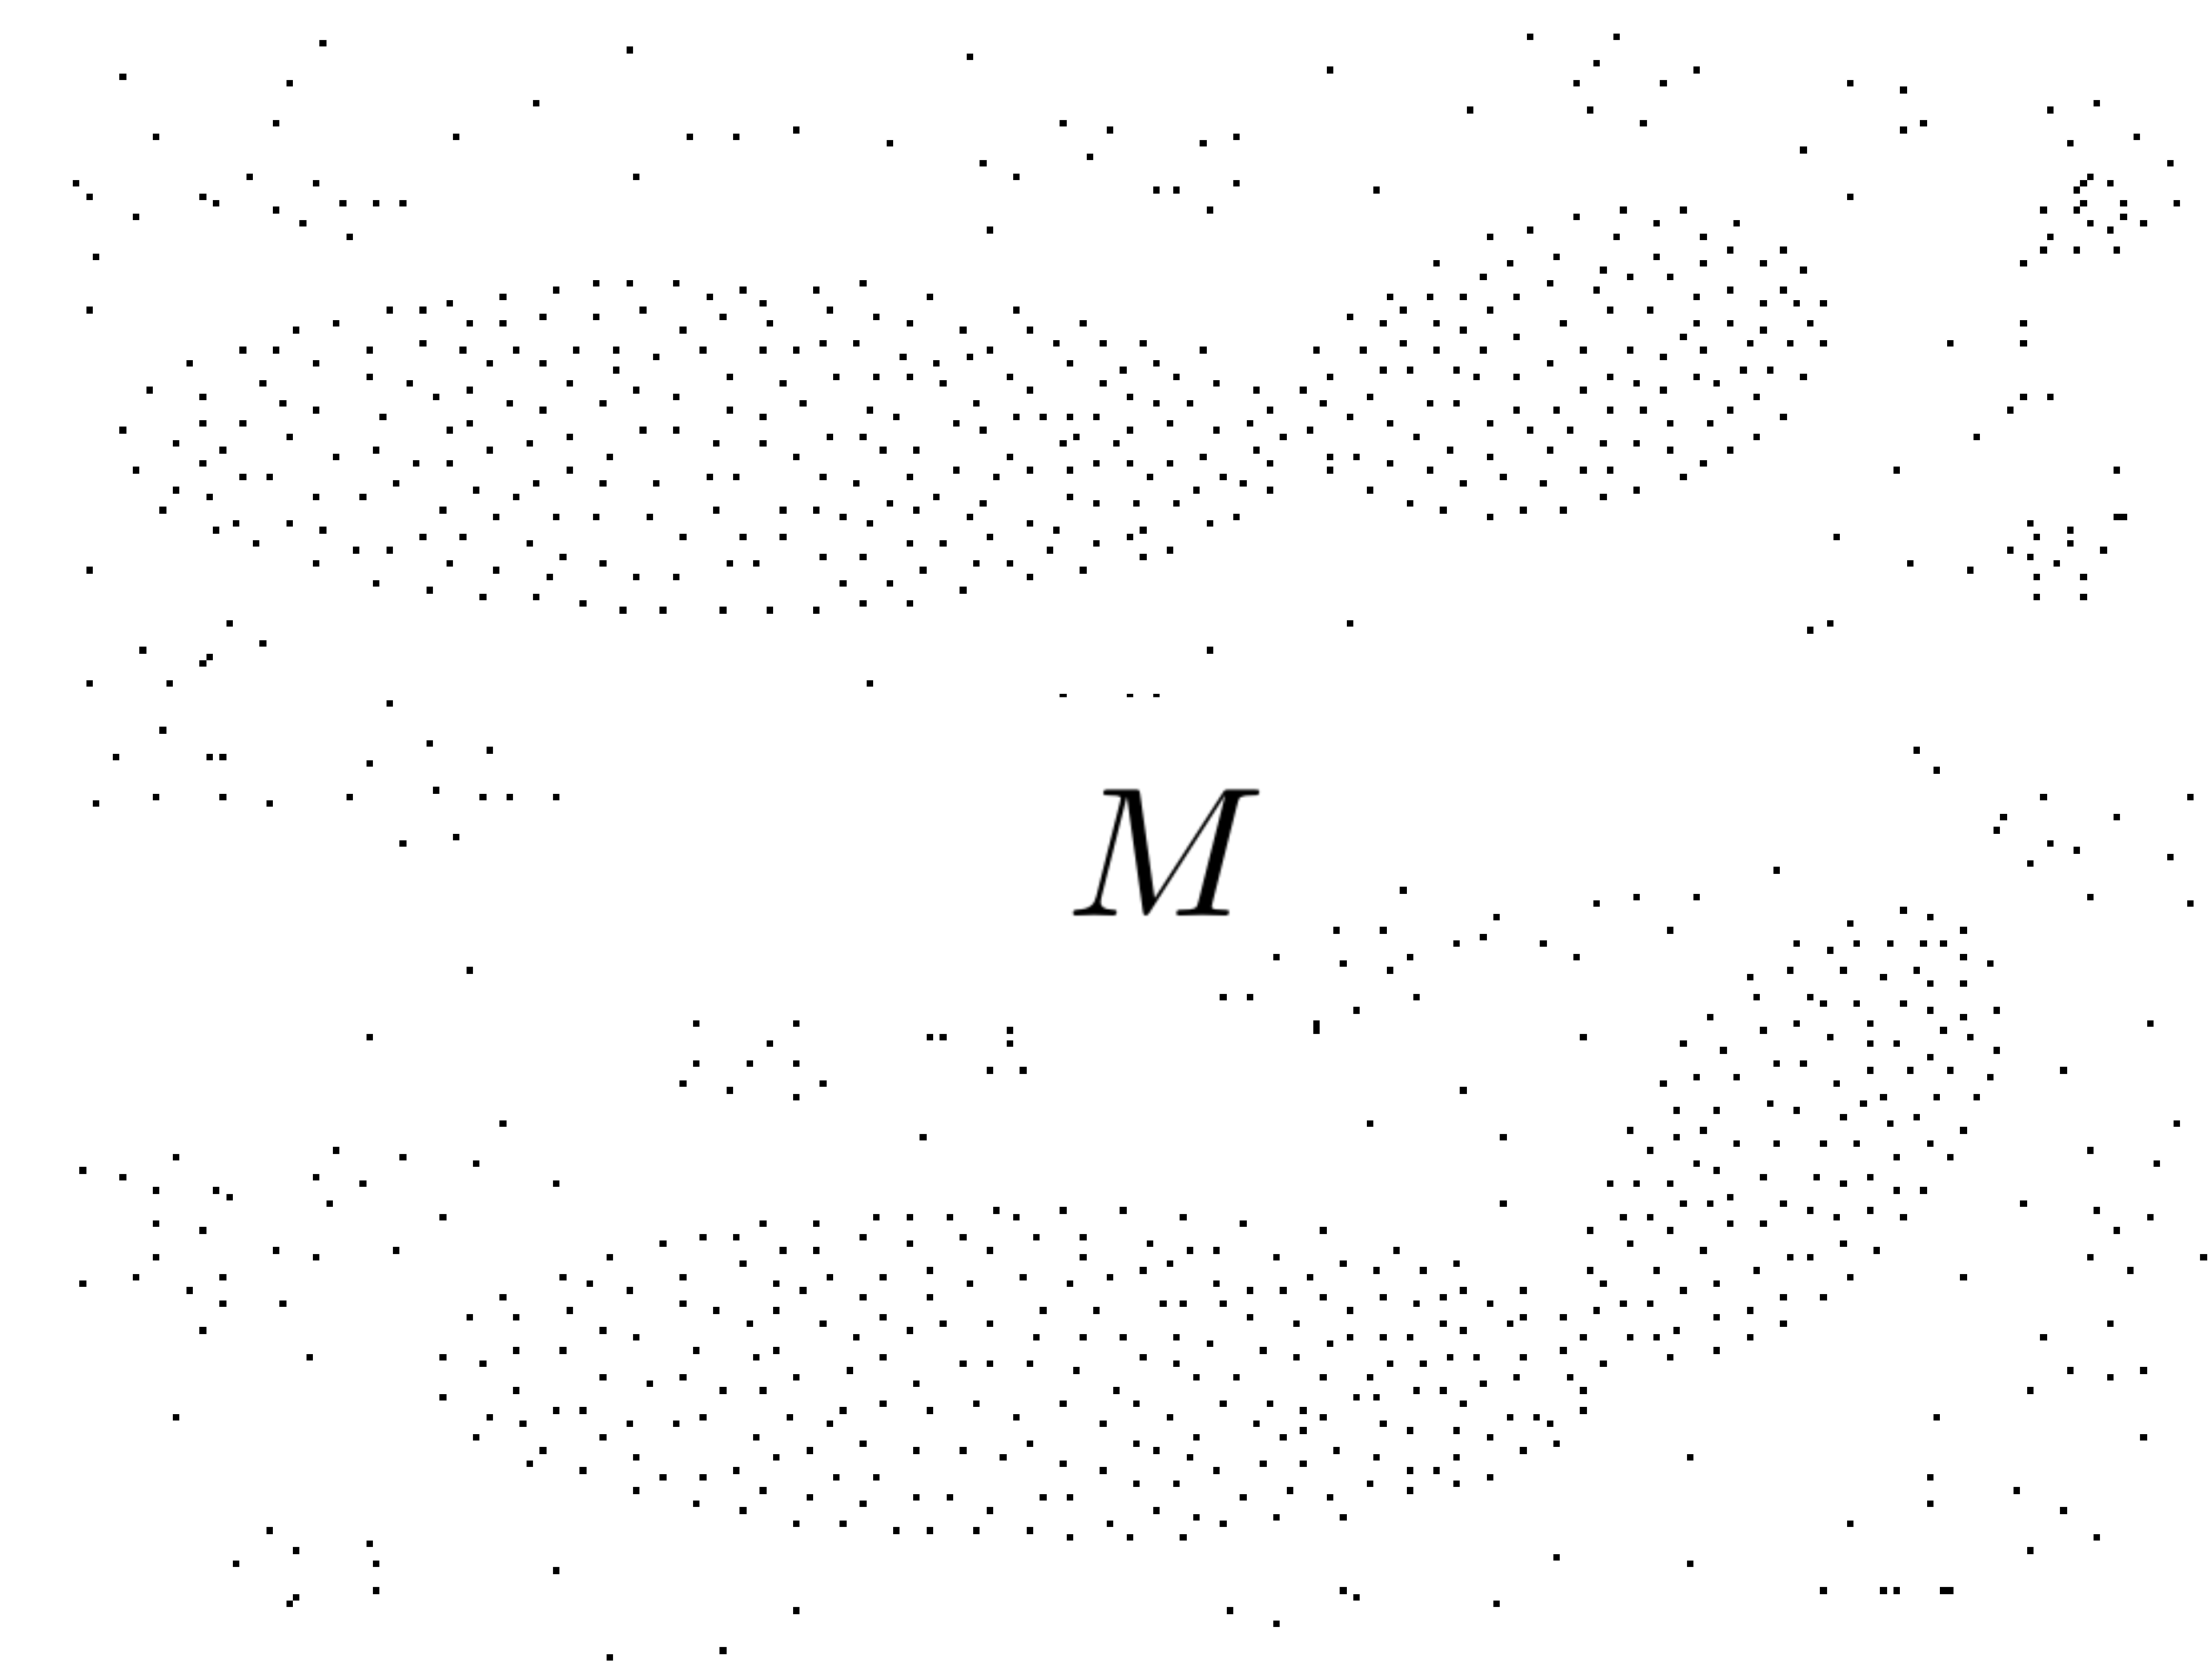
\includegraphics[width=0.45\textwidth]{pc_2parts_Noise}} &		
		\fbox{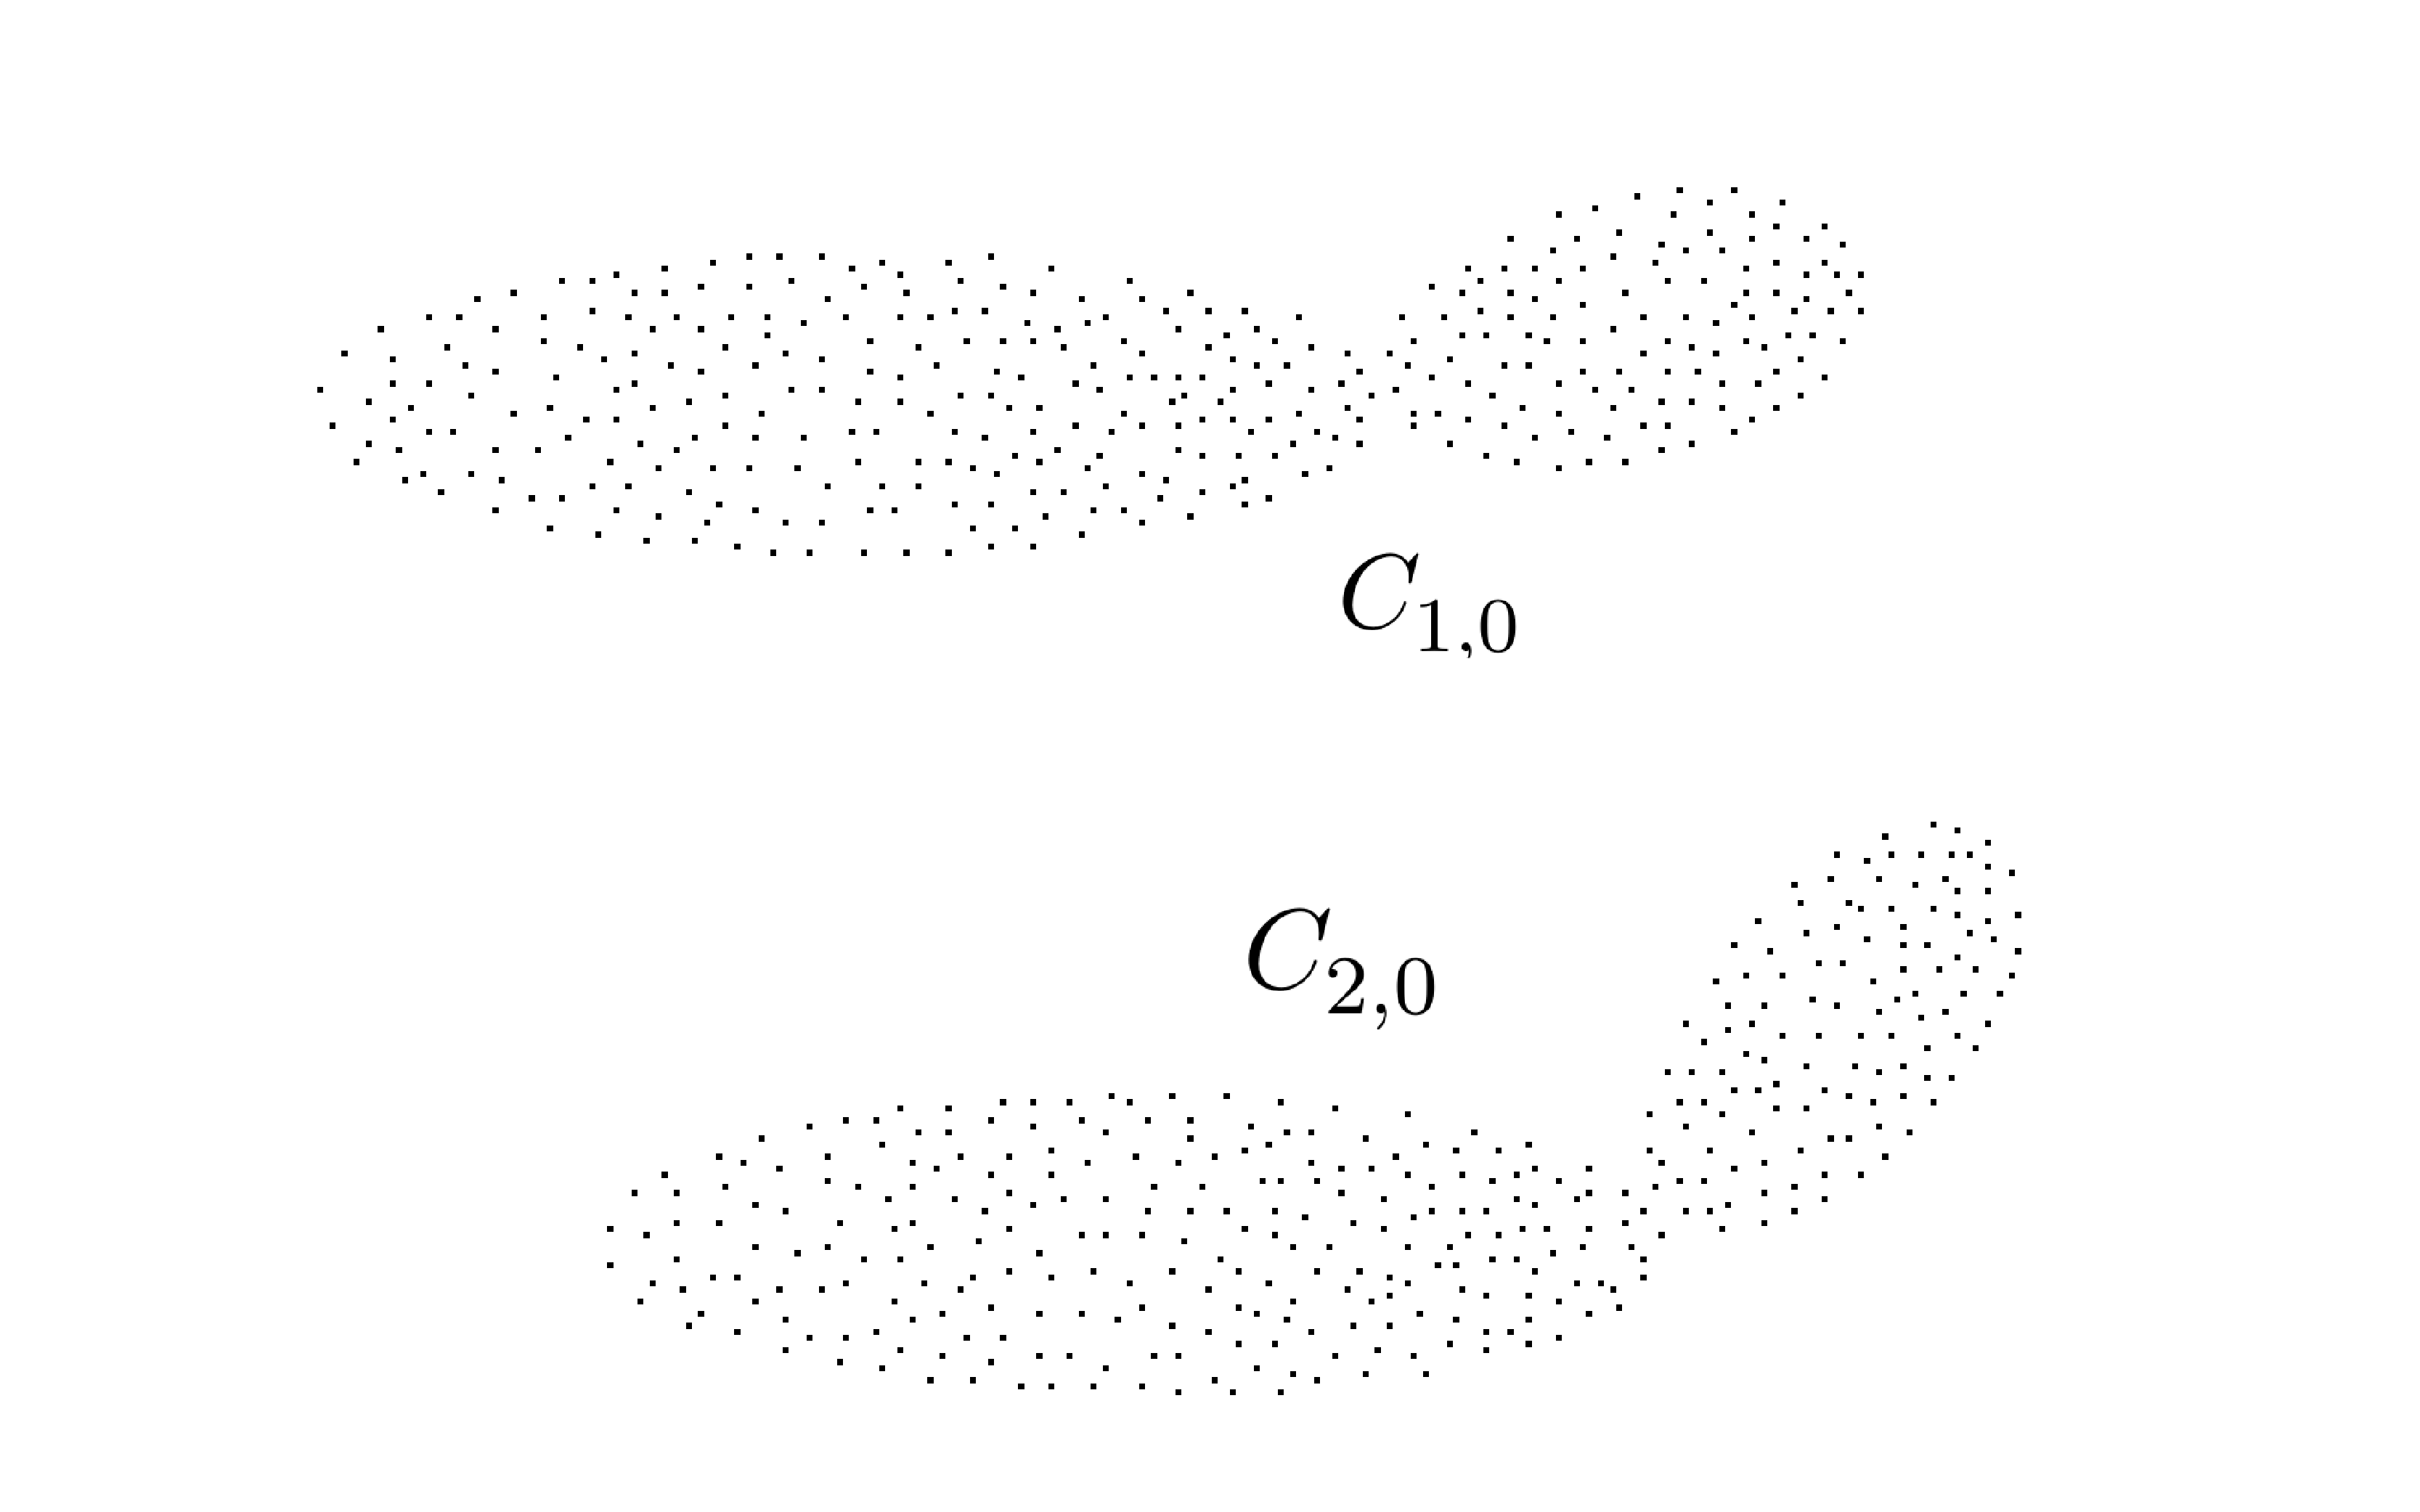
\includegraphics[width=0.45\textwidth]{pc_2parts_noNoise}} 
		\\
		(a) & (b) 
	\end{tabular}
	\caption{Taking a mesh $M$ in two different poses as input (a), removing noise of the input point clouds (b) to achieve the input clusters $C_1$ and $C_2$.} 
	\label{fig:pc_2parts}
\end{figure}

\subsection{Subdividing into clusters}
\label{Subdividing}

As a next step, the two main clusters $C_1$ and $C_2$ are taken as input for further computation steps. If the matching between two clusters does not succeed, they are both subdivided into two sub clusters. Otherwise, no subdividing is done. The whole procedure is repeated recursively for all clusters $\mathcal{C} = (C_{i,1}, \ldots, C_{i,m})$ of $C_1$ and $C_2$ until all associated clusters of $C_1$ match the clusters of $C_2$.  

\subsubsection{Divider position}

To determine where to divide a cluster, it is taken advantage of the principal component analysis (PCA). As a first step, the orientation $\theta$ of $C_1$ and $C_2$ are computed by calculating the central moments
%%
\begin{equation}
	\mu_{pq}(\mathcal{R}) = \sum_{(u,v)\in\mathcal{R}} (u - \bar{x})^p \cdot (v - \bar{y})^q
\end{equation}
%%
\begin{equation}
	\theta(\mathcal{R}) = \frac{1}{2} \tan^{-1} \left(\frac{2\cdot \mu_{11}(\mathcal{R})}{\mu_{20}(\mathcal{R}) - \mu_{02}(\mathcal{R})}\right)
\end{equation}
%%
for each cluster.	
The divider positions are determined by computing the principal axes $p_{1}$ and $p_{2}$ and subsequently taking the perpendicular secondary axes $s_{1}$ and $s_{2}$ through the centroids (see figure \ref{fig:dc_axes_2p}). The secondary axes divide $C_1$ and $C_2$ into the sub clusters $C_{1,1}$ and $C_{1,2}$ as well as $C_{2,1}$ and $C_{2,2}$.

\begin{figure}
	\centering
	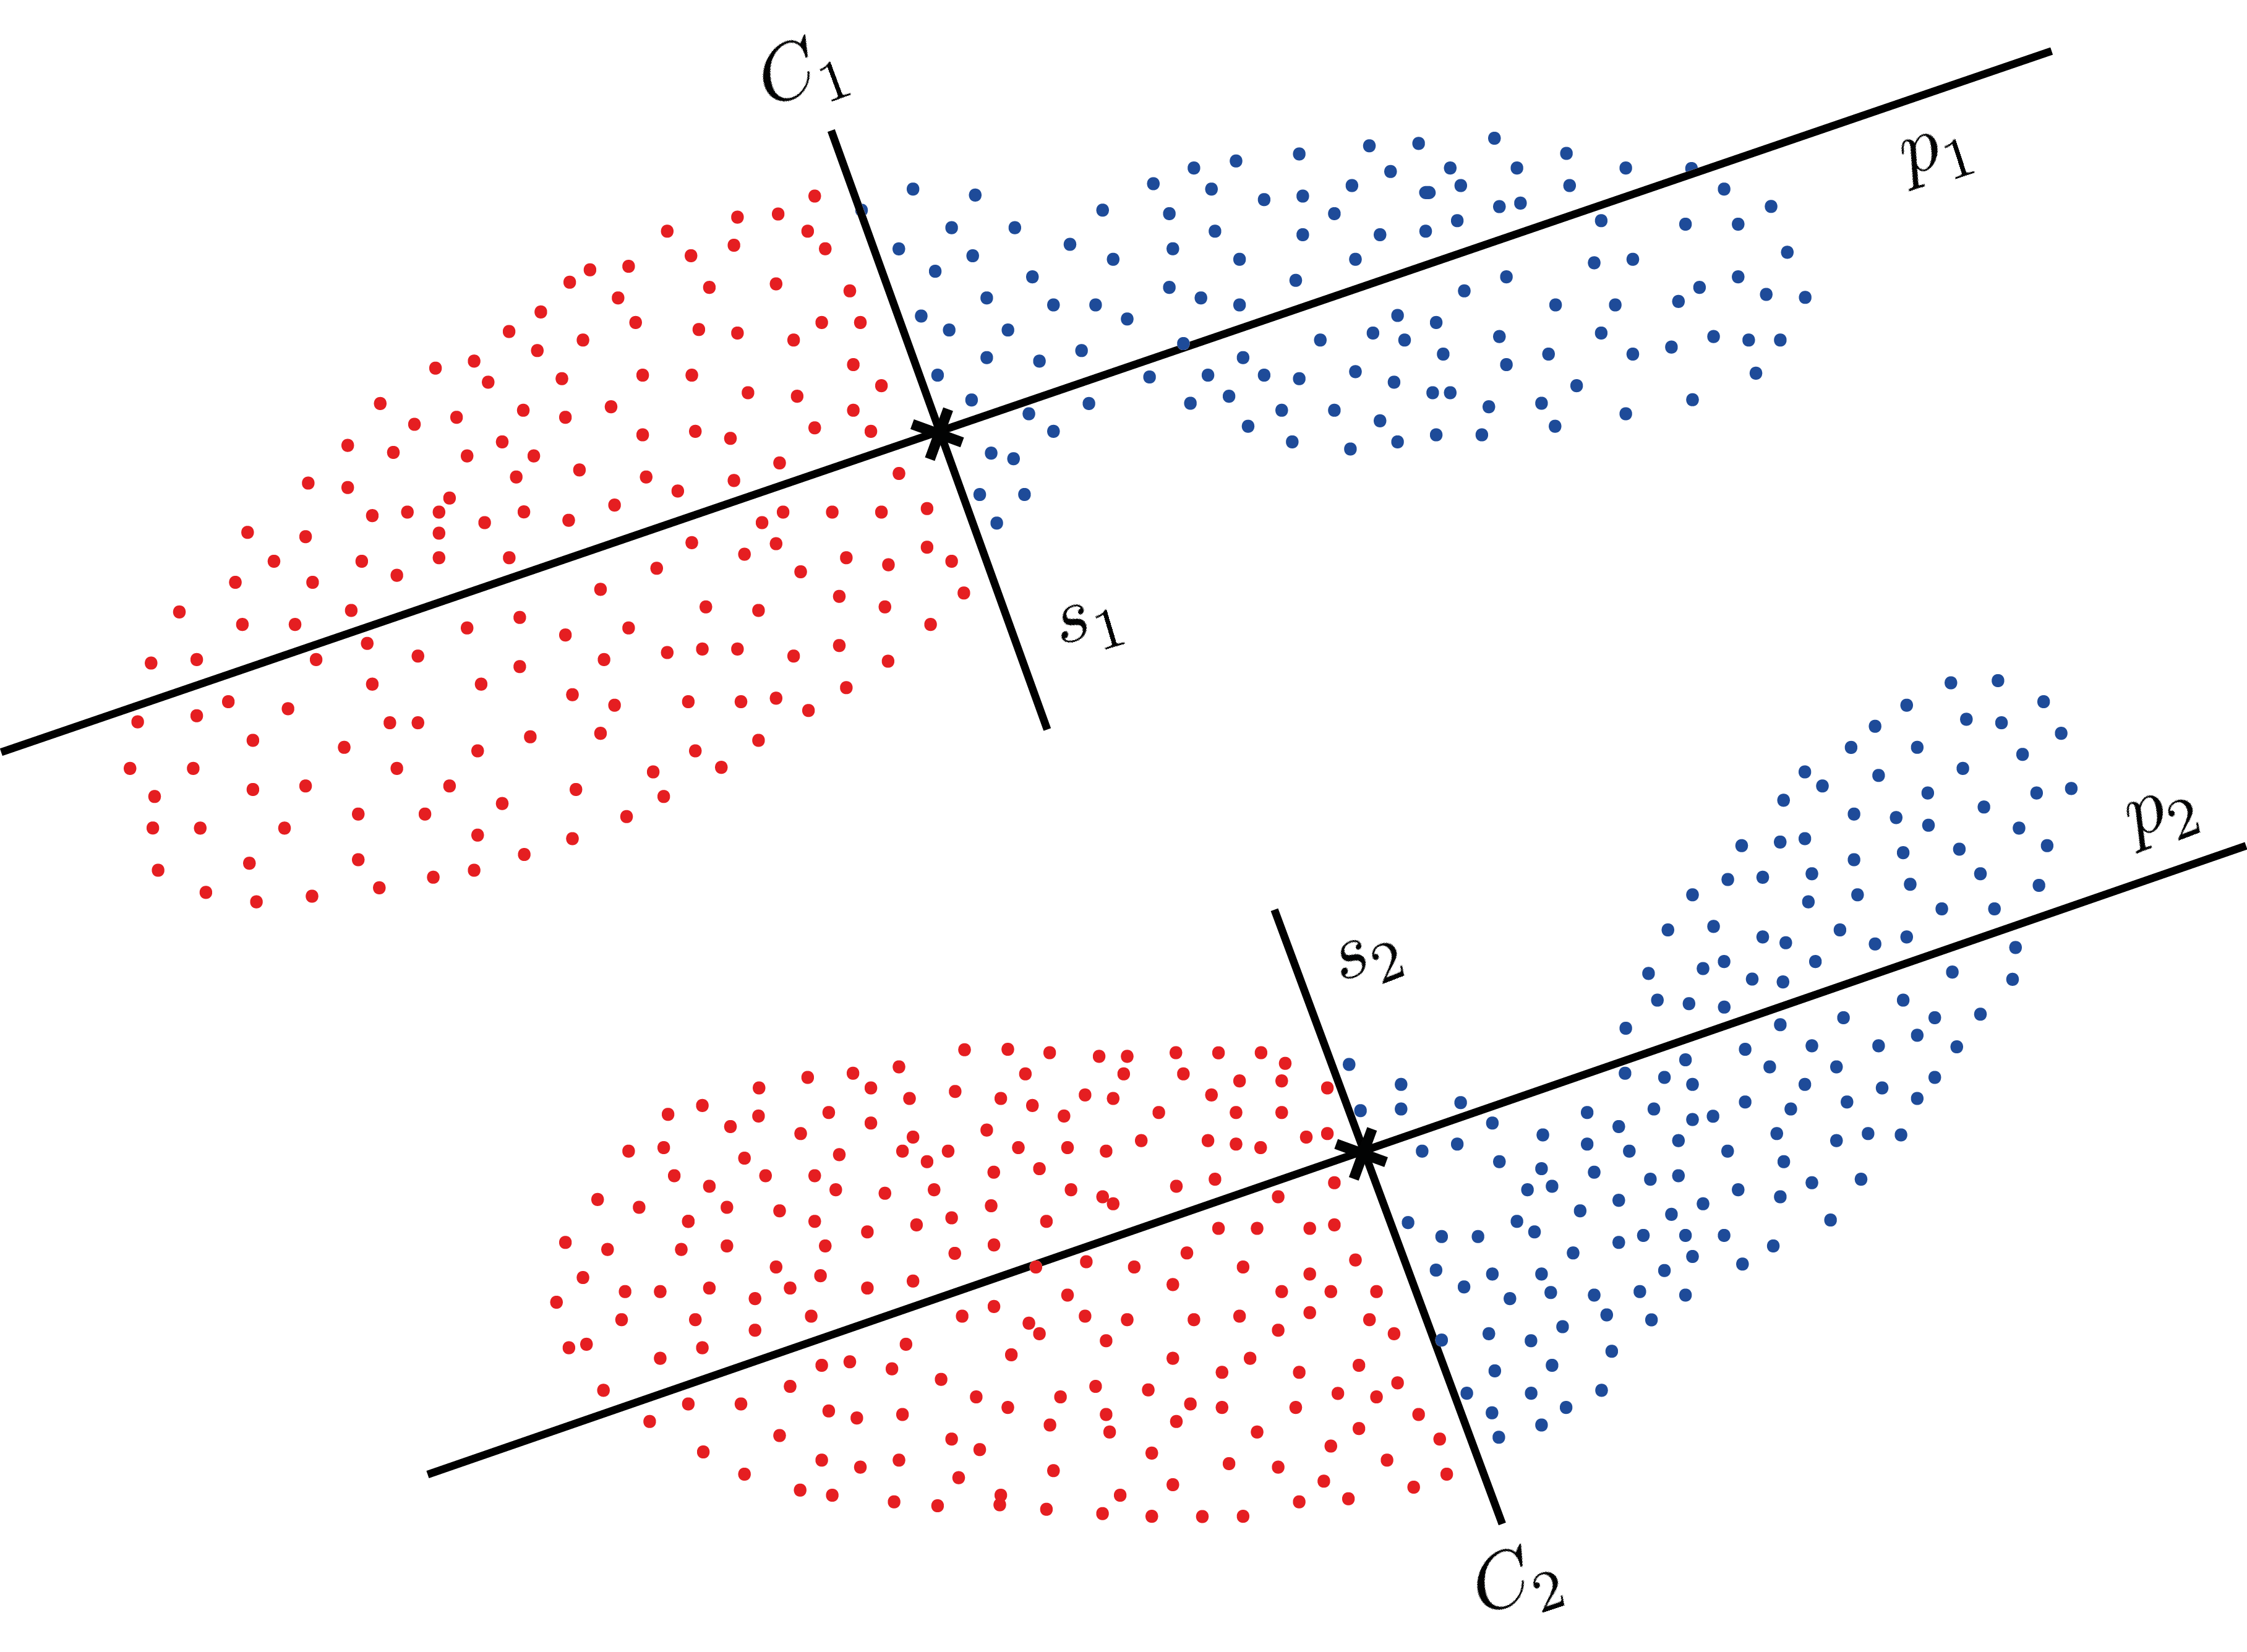
\includegraphics[width=0.8\linewidth]{illustration_axes}
	\caption{Subdividing $C_1$ and $C_2$ into two sub clusters by computing the secondary axes $s_1$ and $s_2$ perpendicular to $p_1$ and $p_2$ through the centroids.}
	\label{fig:dc_axes_2p}
\end{figure}

\subsubsection{Declaring the matching condition between two clusters}

By applying the ICP and the nearest neighbor approach on two associated clusters $C_1$ and $C_2$, a certain matching error $e$ is computed between their cluster points $ C_p =  \{ p_1, \ldots, p_m\}$ and the associated points $ C_q =  \{ q_1, \ldots, q_m\}$. To eliminate the dependency between the matching error and the number of cluster points $m$, the average error per point of $C_p$ and $C_q$
%
\begin{equation}
	e_{\mathrm{avg}(C_p, C_q)} = \frac{1}{| C_p |} \cdot \displaystyle\sum_{i=0}^{m}\| \boldsymbol{p}_i - \boldsymbol{q}_i\|^2
\end{equation}
%
is computed, assuming that the two clusters $C_p$ and $C_q$ contain the same number of cluster points $m$. In case of varying point amounts, the segmentation needs to be carried out differently that sub clusters contain the same number of points. Alternatively, extra points are not considered in the error amount calculation. To declare when two clusters match, it is quite essential to determine an appropriate threshold $\tau$ for the maximum distance $d(p_0, q_0)$ between two associated points $p_0$ and $q_0$. In case of being overvalued, clusters are more likely to match which could result in insufficient subdividing. On the other hand, the clusters are difficult to be matched, which will result in further subdividing and the detection of too many rigid parts. The two clusters $C_p$ and $C_q$ are matching, if $e_{avg} < \tau$.

\subsubsection{Cluster tree}
\label{tree}

The subdividing of the clusters $C_1$ and $C_2$ is realized by a depth-first approach in a tree. Consequently, $C_1$ and $C_2$ represent the root and are subdivided from the left to the right. A node $N$ of the tree contains two related clusters $C_{1,i}$ and $C_{2,i}$, where $i$ defines whether the node is a left ($i=1$) or right ($i=2$) node of the parent. In case of further subdividing, a Node $\mathit{left}$, containing the  clusters $C_{1,i,1}$ and $C_{2,i,1}$, as well as a Node $\mathit{right}$, containing the clusters $C_{1,i,2}$ and $C_{2,i,2}$ origin. If two associated clusters $C_{1,i,j}$ and $C_{2,i,j}$ in a Node $N_i$ match, no further subdividing is performed. The resulting leaves of the tree are the final matching sub clusters and stored from left to right in a list $\mathcal{L} = (L_{1,1},L_{2,1},\ldots,L_{1,m},L_{2,m})$ (see figure \ref{fig:illustrationTree}). By applying the depth-first approach, the neighboring clusters in the list are also neighboring clusters in the main clusters $C_1$ and $C_2$.  As a result, in the following step the adjacent sub clusters of $C_1$ or $C_2$ can be merged (see subsection \ref{mergingClusters}).
\begin{figure}
	\centering
	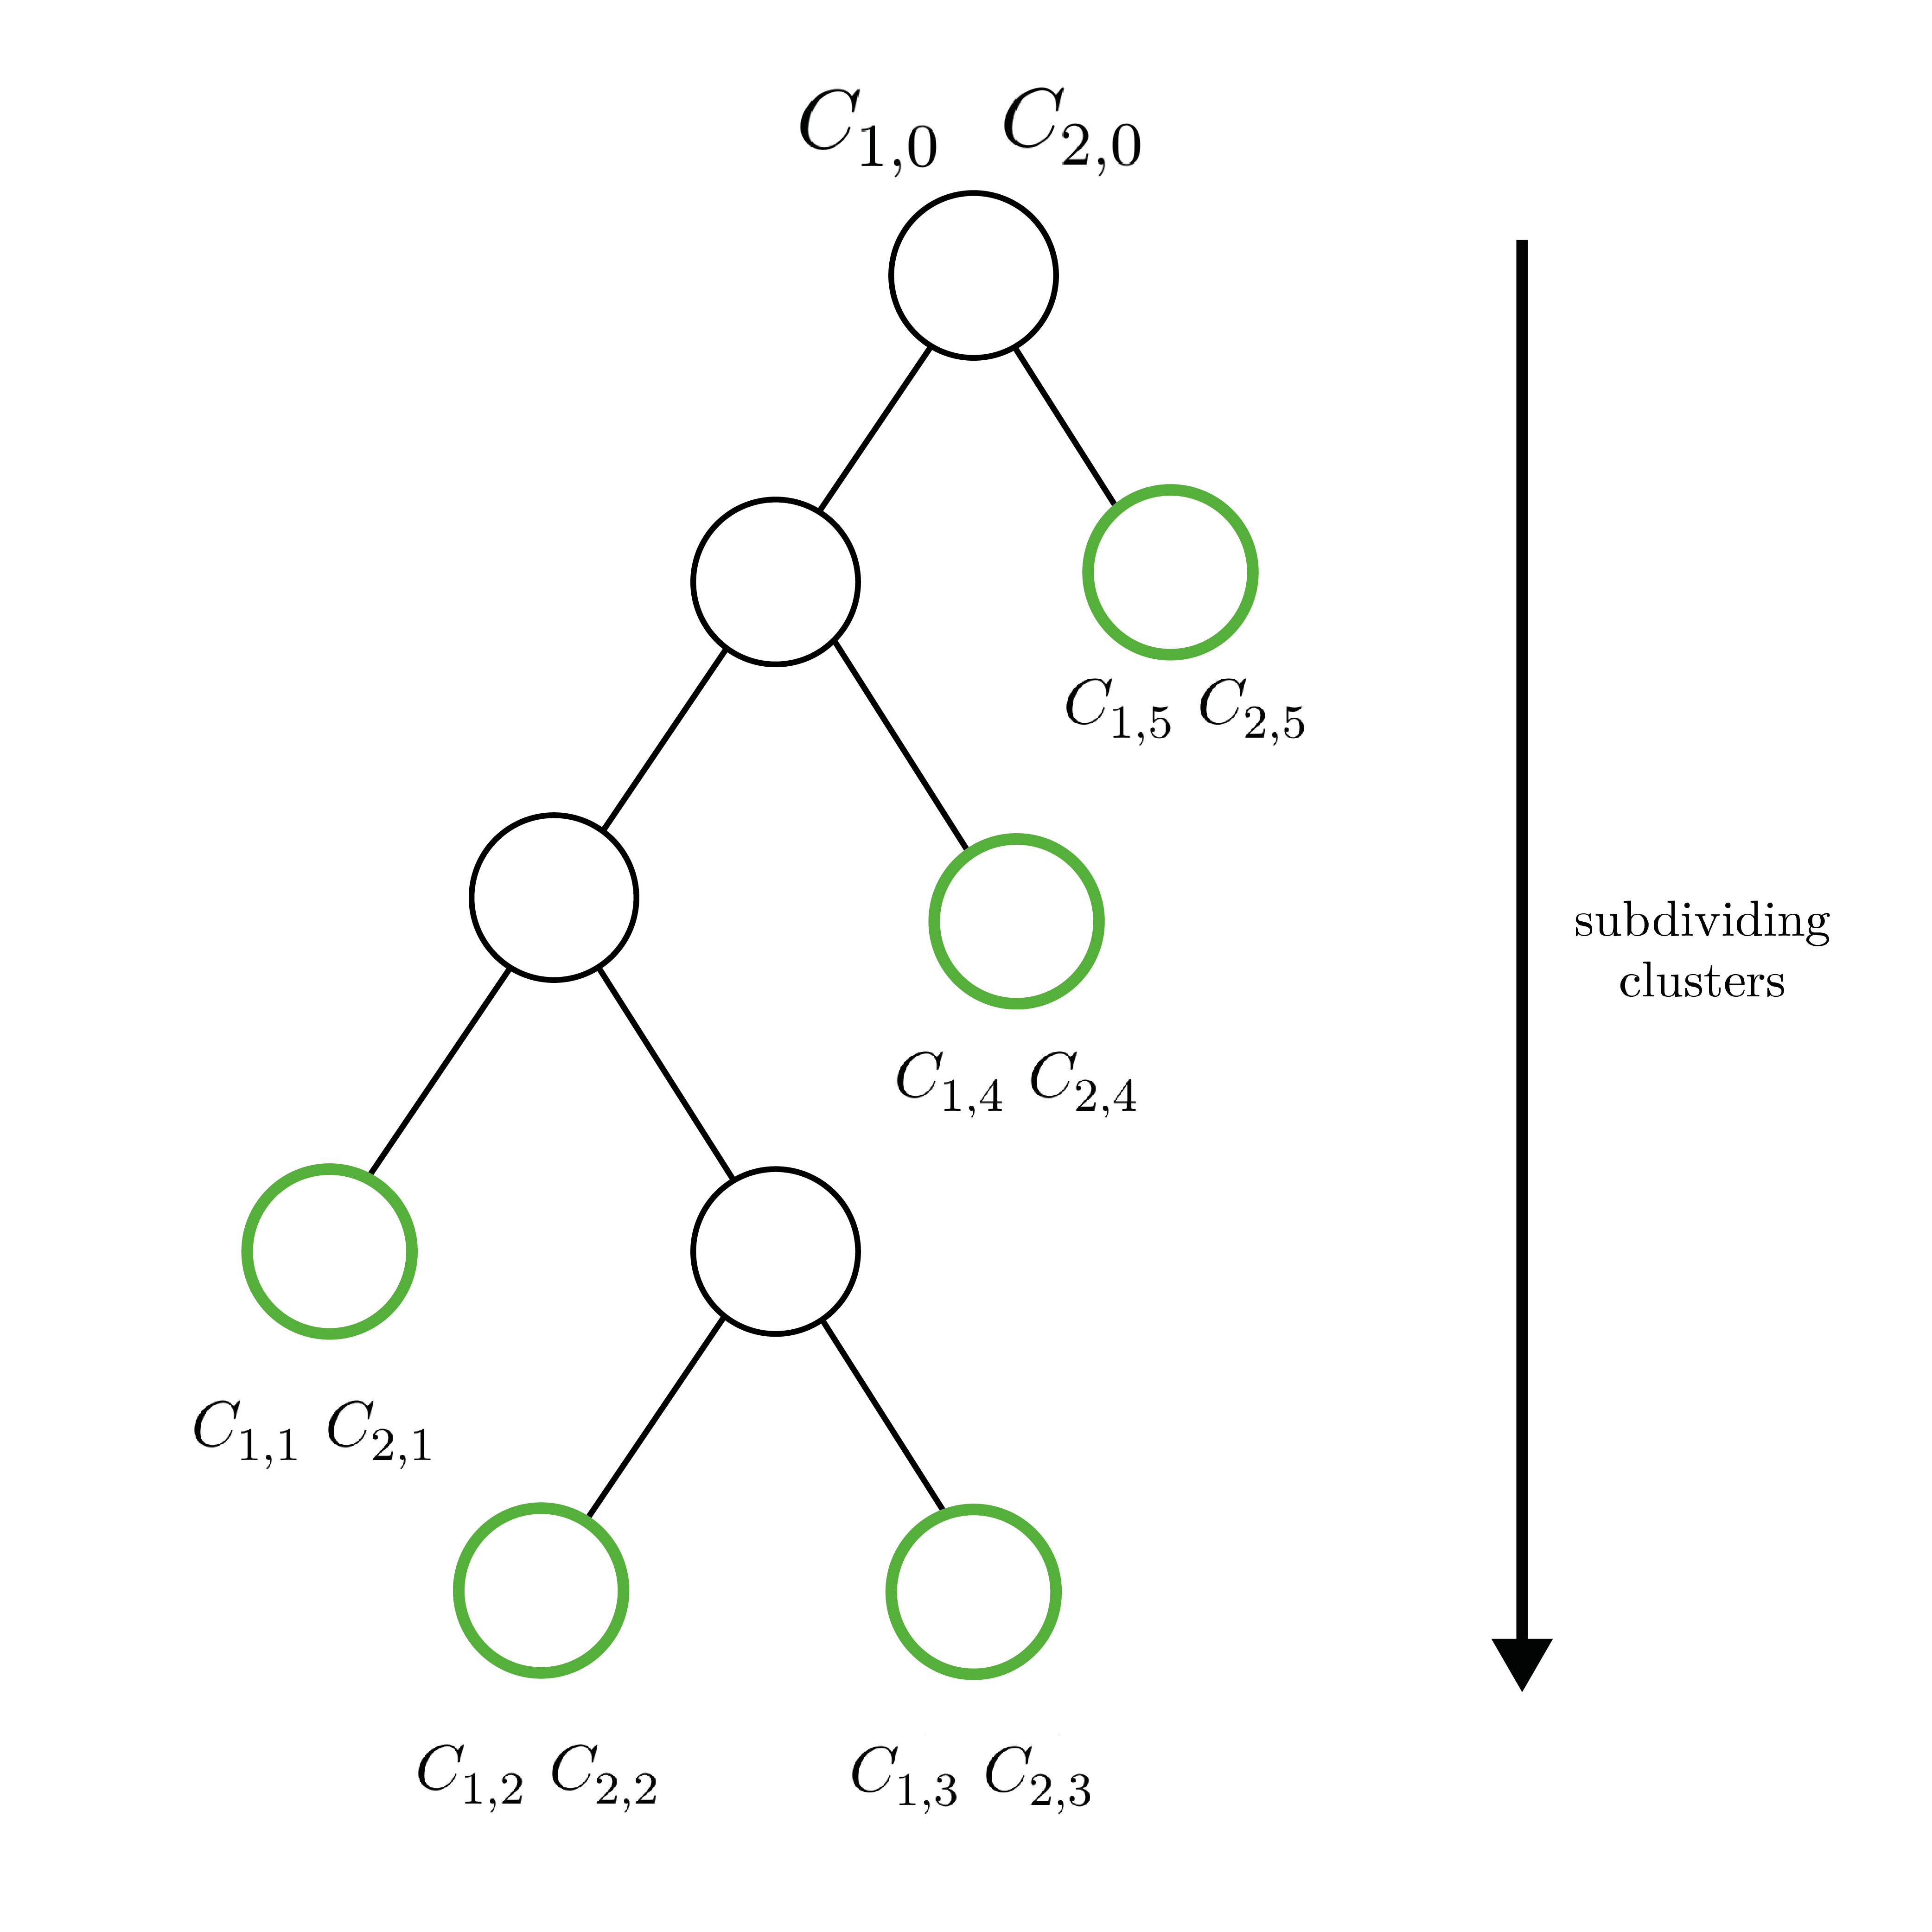
\includegraphics[width=0.7\linewidth]{IllustrationTree}
	\caption{Subdividing of $C_1$ and $C_2$ into matching clusters by a depth-first approach in a tree. The Subdividing terminates if all sub clusters of $C_1$ and $C_2$ match when applying the ICP.}
	\label{fig:illustrationTree}
\end{figure}

\subsection{Merging neighboring clusters to rigid parts}
\label{mergingClusters}x
%%
As a next step, adjacent sub clusters from $\mathcal{L}$ are iteratively merged and subsequently verified to still match. This process is required to rejoin, if necessary, detected sub clusters to the rigid parts of the object. This is the case, if a rigid part was subdivided during the subdividing process (see section \ref{Subdividing}). The merging initiates with the first clusters in the list $L_{1,i}$, $L_{2,i}$ and its adjacent clusters $L_{1,i+1},L_{2,i+1}$. If the resulting merged clusters can be matched, the merging proceeds with the adjacent cluster $L_{1,i+2},C_{2,i+2}$. If not, the merging is not executed and $L_{1,i}$, $L_{2,i}$ are stored in a list of resulting clusters $\mathcal{R}$. The merging procedure then initiates with $L_{1,i+1},L_{2,i+1}$. The process terminates if all clusters of $\mathcal{L}$ are verified and consequently the clusters of $\mathcal{R}$ are assigned to rigid parts $\mathcal{P} =  \{P_1,\ldots,P_m\}$ (see figure \ref{fig:clusterChain}). 

\begin{figure}
	\centering
	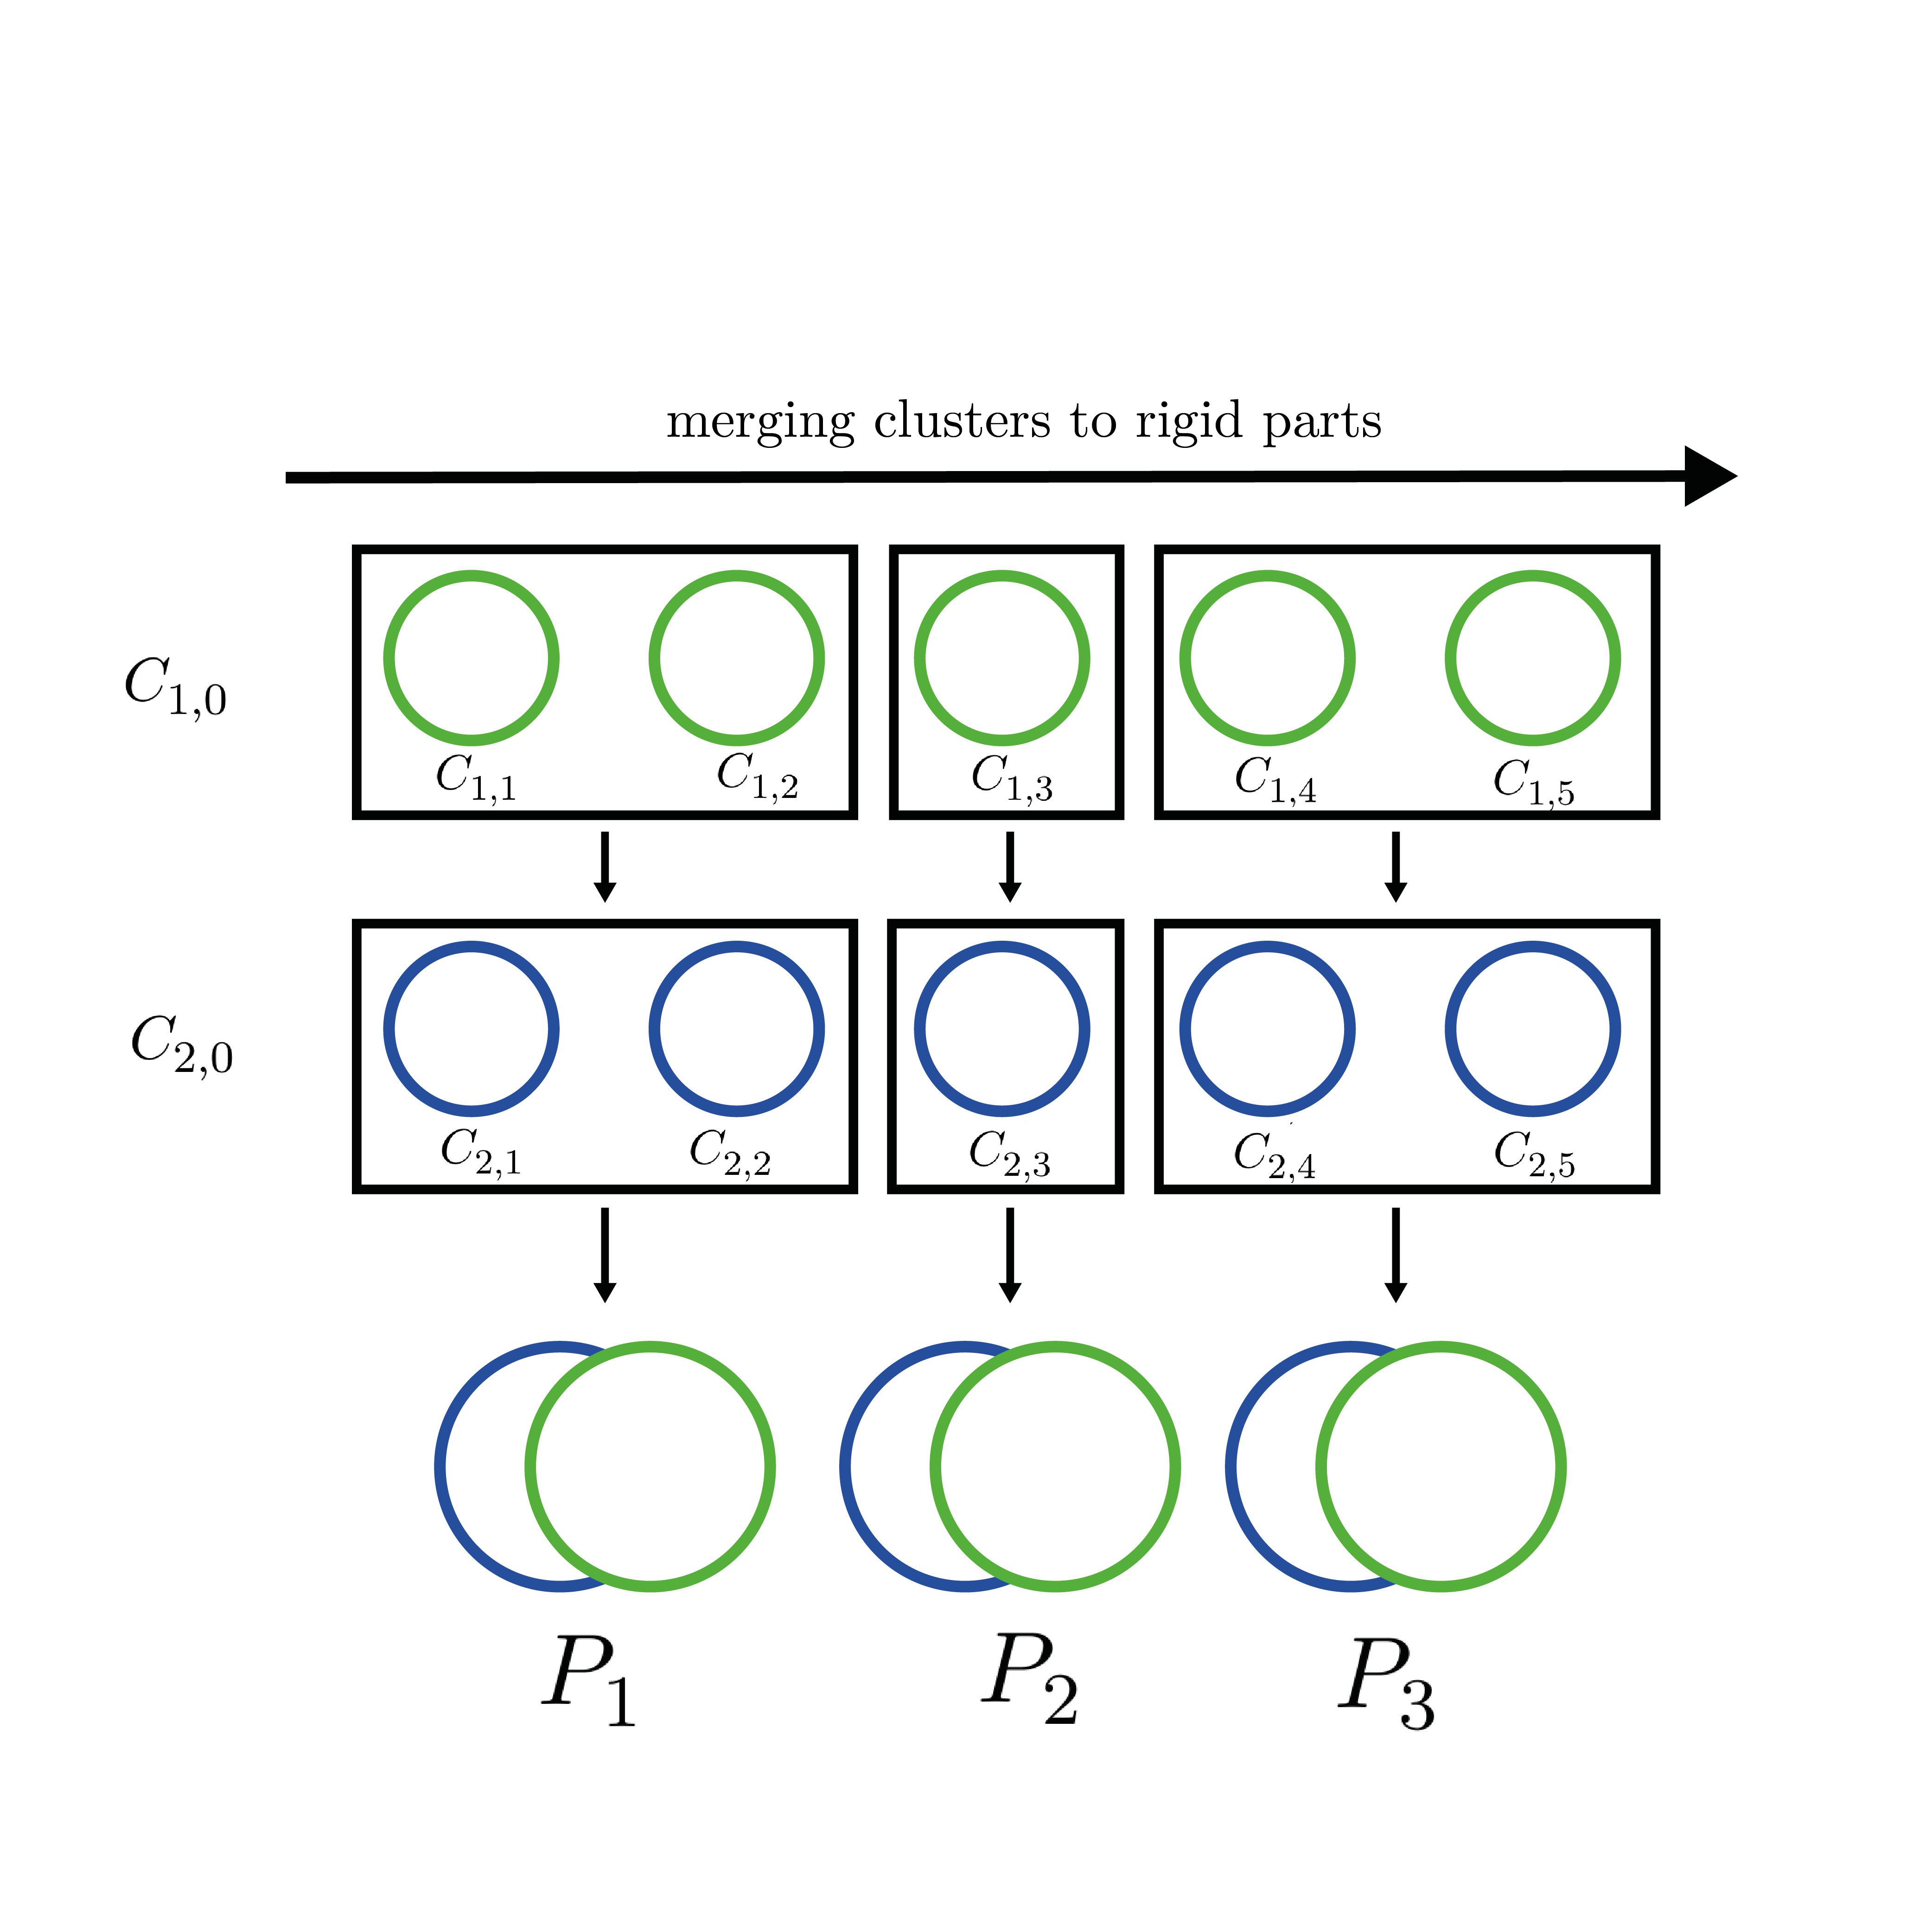
\includegraphics[width=0.8\linewidth]{ClusterChain}
	\caption{Detecting rigid parts of $C_1$ and $C_2$ by iteratively merging adjacent clusters of $\mathcal{L}$ that merged clusters still match.}
	\label{fig:clusterChain}
\end{figure}

\subsection{Joint/skeleton estimation}

After detecting the rigid parts $\mathcal{P} =  \{ {P_1,\ldots,P_m}\}$, they are linked with joints. Their locations are thereby calculated by computing the points of intersection of all principal axis of $\mathcal{P} = \{ {P_1,\ldots,P_m}\}$. However, this calculation assumes that the rigid parts are symmetric, as in the other case the principal axis might not represent the skeleton of an object. For this reason another approach has to be taken into account. Anguelov \cite{Anguelov04} declares joints as two points of two neighboring rigid parts that undergo the same transformation $T$. In the current implementation an object point is only allocated to one rigid part $P$. An improvement of the current situation is therefore to select points that are located near a joint allocated to more neighboring rigid parts and from those selected points the location of a joint is computed. 

\begin{figure}[H]
	\centering\small
	\begin{tabular}{cc}
		\fbox{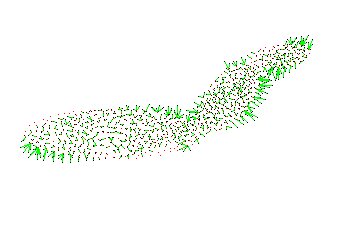
\includegraphics[width=0.45\textwidth]{results/non-rigid_3parts_associations}} &
		\fbox{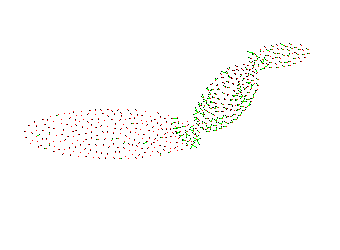
\includegraphics[width=0.45\textwidth]{results/rigid_3parts_associations}} 
		\\
		(a) & (b) 
	\end{tabular}
	\caption{Registration of $C_1$ and $C_2$ before the segmentation into rigid parts (a) and after the segmentation.} 
	\label{fig:ICPResults}
\end{figure}

\section{Implementation}

After planning the algorithm, it was initially implemented and for 2D point clouds, in order to be able to focus solely on developing and testing.

\subsection{Chosen environment}

The initial approach was implemented in Java, using ImageJ as processing library. The chosen environment depends on the following factors:
\begin{itemize}
	\item familiarity and prior experience
	\item complexity
	\item available plug-in for image processing
\end{itemize}
%%
As ImageJ is mainly used for 2D use cases, another implementation would be possible in 3D using PCL in C++. As a result, the attention can be brought to segmentation and visualization in 3D.

\subsection{Architecture}

The initial algorithm was realized with four classes to divide the ``divide and conquer'' algorithm from the Cluster object as well as the Visualization and the registration process of sub clusters.
The main class \texttt{Segmentation} solely requires a stack of two point clouds in 2D. As a first step, possible noise is removed from the input mesh $M$ (see algorithm \ref{alg:noiseRemoval}). The algorithm returns the biggest point cluster $C_i$ that is assumed to be an articulated object. A class \texttt{Cluster} was implemented to store the cluster's points, its centroid, the orientation $\theta$ as well as the principal and secondary axes. For the subdividing, a \texttt{ClusterTree} was implemented to simultaneously divide the main clusters $C_1$ and $C_2$ into sub clusters (see algorithm \ref{alg:subdivide}). Each node $N$ contains thereby two associated clusters $C_{1,i}$ and $C_{2,i}$. For the clustering and merging of clusters a \texttt{List<Clusters>} was used to dynamically add and remove Clusters. Furthermore, a class \texttt{ICP} was created, which takes two clusters to be matched as input, using Procrustes fitting. First, the noise removal and cluster detection is done in the \texttt{Cluster} class. As a next step, the detected main clusters $m$  $C_1,\cdots,C_{m}$ are taken as input with an empty list to get the matching sub clusters of all input clusters. Following, the divide and conquer algorithm (see algorithm \ref{alg:subdivide}) takes advantage of the ICP class to iteratively register two sub clusters of two main clusters $C_{i},\cdots,C_{j}$. As the segmentation is done depth first the verified sub clusters are stored in the list from left to right. The returned segmented list is taken as input to iteratively merge the sub clusters to detected rigid parts (see algorithm \ref{alg:merging}). As a return we get a list with sub clusters representing the rigid parts of the input clusters. Subsequently, the Visualization class is used, to color the cluster points differently and draw PCA related components, like the axis and interference points of different rigid parts.

%TODO: add code snippets for Procrustes, explain ICP...

\subsection{ICP}
One main part of the algorithm is the modified implementation of the ICP using Procrustes fitting to compute a transformation that detects sparse point correspondences. Thereby, only reciprocal correspondences within a specific distance $\tau$ contribute to the calculation. The final point correspondences of $C_i$ and $C_j$ are stored in a \texttt{Map<Integer, Integer>} containing the indices of the corresponding points. This is because the storage of points in the form $\boldsymbol{p}_i(x,y)$ would underly a specific transformation, which is applied during the ICP and initial alignment. For further computations using the RANSAC, no transformations are desired. As the main difficulty is the right initial alignment of the actual largest rigid part (torso) the value of the distance threshold $\tau$ is chosen generously. As a result, a higher number of false point correspondences is detected which has to be compensated by RANSAC (see subsection \ref{RANSAC}).

\begin{lstlisting}
...
for (Map.Entry<Integer, Integer> entry : reference.entrySet()) {
Integer referenceIndex = entry.getKey();
Integer targetIndex = entry.getValue();

if (target.containsKey(targetIndex) && target.get(targetIndex) == referenceIndex) {
referencePoints.add(originalReference.get(referenceIndex));
targetPoints.add(originalTarget.get(targetIndex));
finalAssociations.put(referenceIndex, targetIndex);
}
}
...
\end{lstlisting}

\begin{figure}
	\centering
	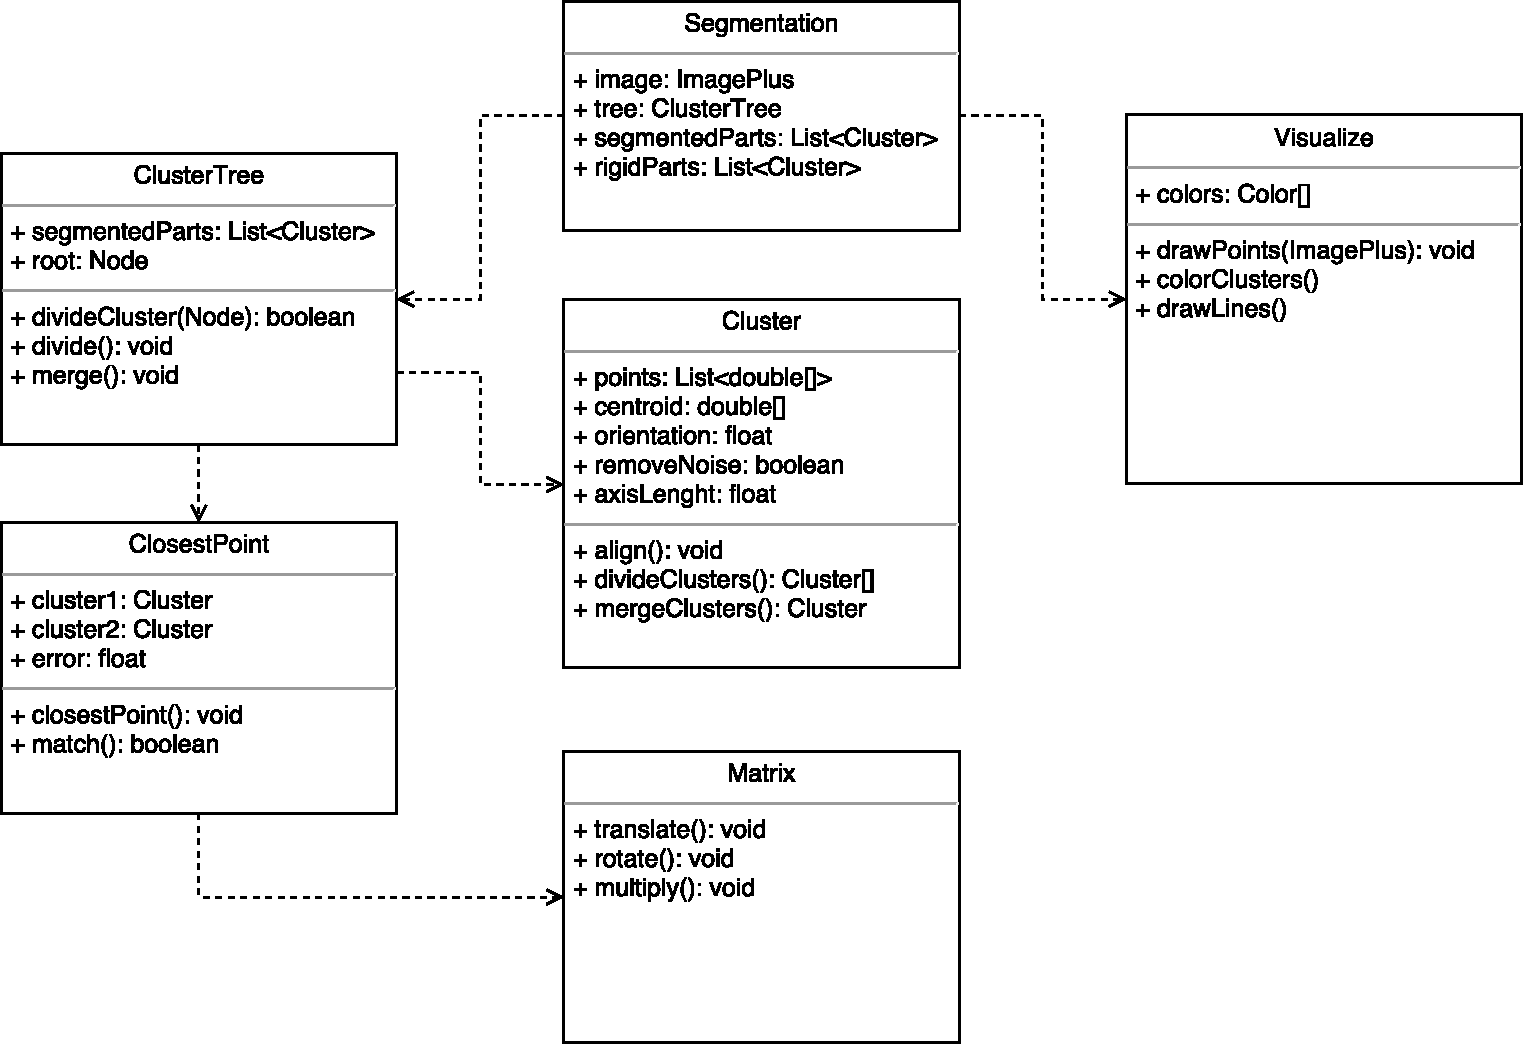
\includegraphics[width=0.9\linewidth]{SegmentationUML}
	\caption{UML diagram of the classes related to the implementation of the algorithm.}
	\label{fig:UML}
\end{figure}

\begin{algorithm}[tbp]
	\caption{Noise removal of an input point mesh $M$ in form a set of unclustered points $\{\boldsymbol{u}_1,\ldots,\boldsymbol{u}_n\}$ by region growing. The first point of $M$ is used as seed and grows a cluster $C_{current}$ by iteratively adding neighboring points located inside a threshold $\tau$. Once, all points have been examined, the largest cluster $C_{max}$ is returned and defined as articulated object to be segmented.}
	
	\begin{algorithmic}[1]     % [1] = all lines are numbered
		\label{noiseRemoval}
		
		\Procedure{RemoveNoise}{$M$} 
		\State $\mathit{C_{max}} \gets ()$
		\State $\mathit{C_{current}} \gets ()$
		\State $n \gets \mathit{sizeOf}(M)$
		\State $m \gets \mathit{sizeOf}(C_{current})$
		
		\While {$n$ > 0}
		\State $\mathit{c_{current}} \gets \mathit{c_{current}} + \boldsymbol{u}_1$
		\For{$i = 1,\ldots,m$}
		\State $M \gets M - C_{current}$
			\For{$j = 1,\ldots,n$}
			\If {\Call{$d$}{$\boldsymbol{p}_i, \boldsymbol{u}_j}< \tau$}
			\State $C_{current} \gets C_{current} + \boldsymbol{u}_j$
			\EndIf
			\EndFor
		\EndFor
		\State $M \gets M - C_{current}$
		\If{$m > \mathit{sizeOf}(C_{max})$}
		\State $C_{max} \gets C_{current}$
		\EndIf
		\State $C_{current} \gets ()$
		\EndWhile
		\State\Return $C_{max}$
		\EndProcedure	
	\end{algorithmic}
\end{algorithm}

\begin{algorithm}[tbp]
	\caption{Recursive subdividing of two clusters $C_1$ and $C_2$, in the form of a Node $\mathit{N}$ in a Tree, into matching sub clusters. The ICP is applied on two corresponding clusters in $\mathit{N}$ to verify them to match, in which case they are stored in a list. Otherwise, if the two clusters do not match, they are further subdivided. The list with all matching subclusters is returned once the subdivide algorithm terminates.}
	\label{alg:subdivide}
	
		\begin{algorithmic}[1]     % [1] = all lines are numbered
			\label{clusterTree}
			\Procedure{ClusterTree}{$\mathit{C_1}, \mathit{C_2}$}
			
			\State $L \gets ()$
			\State $\mathit{left} \gets \mathit{nil}$
			\State $\mathit{right} \gets \mathit{nil}$
			\State $N \gets \langle C_1, C_2, \mathit{left}, \mathit{right}\rangle$
			\State $L \gets \Call{Subdivide}{N}$
			\State $P \gets \Call{MergeClusters}{L}$
			
			\EndProcedure
		\end{algorithmic}
	
	\begin{algorithmic}[1]     % [1] = all lines are numbered
		\label{subdivide}
		\Procedure{Subdivide}{$N$}
		
		\If {$\Call{match}{C_1(N)}, C_2(N)$}
		\Comment{Apply ICP on two clusters}
		\State $L \gets L + (N)$
		
		\Else
		\State $\mathit{left}(N) \gets \Call{Split}{N}$
		\State $\mathit{right}(N) \gets \Call{Split}{N}$
		\Comment{Split the cluster into a left and right side}
		\State \Call{Subdivide}{$\mathit{left}(N)$}
		\State \Call{Subdivide}{$\mathit{right}(N)$}
		\Comment{Recall the algorithm with sub clusters}
		\EndIf
		
		\State\Return $L$
		\Comment{Return all sub clusters after termination.}
		\EndProcedure
			
	\end{algorithmic}
\end{algorithm}

\begin{algorithm}[tbp]
	\caption{Merging of the sub clusters $\mathit{L} = ((L_{1,1}, L_{2,1}),\ldots,(L_{1,m}, L_{2,m}))$, resulting from algorithm \ref{alg:subdivide} in the order of being stored, to rigid parts $\mathcal{P}$. Verify the matching of merged adjacent clusters $L_{i,j}$ and $L_{i,j+1}$ from $C_1$ and $C_2$. The merging is continued until no match can be done. In this case the last last merged cluster pairs are stored as rigid parts $P_1$ and $P_2$. The algorithm then continues with the next cluster pair in the list and terminates if all pairs have been traversed. The list with all detected rigid parts $\mathcal{P}$ is returned.}
	\label{alg:merging}
	
	\begin{algorithmic}[1]     % [1] = all lines are numbered
		\label{merging}

		\Procedure{MergeClusters}{$L$} 
		\State $P \gets ()$
		\State $P_1 \gets L_{1,1}$
		\State $P_2 \gets L_{2,1}$
		\State $n \gets \mathit{sizeOf}(L)$
		
		\For{$i = 2,\ldots,n$}
		\State $\mathit{merge_1} \gets \Call{Merge}{P_1, L_{1,i}}$
		\State $\mathit{merge_2} \gets \Call{Merge}{P_2, L_{2,i}}$
		
		\If {\Call{match}{$merge_1$, $merge_2$}}
		\Comment{Apply ICP on two merged clusters}
		\State $\mathit{P_1} \gets merge_1$
		\State $\mathit{P_2} \gets merge_2$
		\Comment{Continue merging with merged clusters}
		\Else
		\State $P \gets P + (P_1, P_2)$
		\State $P_1 \gets L_{1,i}$
		\State $P_2 \gets L_{2,i}$
		\Comment{Initiate merging with current clusters}
		\EndIf
		\EndFor
		\State $P \gets P + (merge_1, merge_2)$
		\State\Return $P$
		\EndProcedure	
	\end{algorithmic}
\end{algorithm}

\section{Results}

At first, the implementation was tested on two point clouds of an articulated object with only two rigid parts. The segmentation results are directly dependent on the matching error threshold $\tau$ which can bee seen on table \ref{table:segmentation_results}. The higher the threshold $\tau$, the less clusters and subsequently rigid parts can be detected, as two clusters are more likely to match and are not further subdivided. The lower $\tau$, the more clusters and rigid parts will be detected, as clusters require further subdividing in order to match. Figure \ref{fig:2rigidParts} and figure \ref{fig:3rigidParts} show the clustering and rigid part detection of two simple objects, in regard to their rigid parts linked like a chain. For those objects, with a threshold $\tau = 5$ the right number of rigid parts is detected. However, the segmentation position does not correspond to the actual joint of $C_1$ and $C_2$. The reason is, that the average error $e_{avg}$ is computed without any weighting of points. Especially points located near a joint need to be treated cautiously. Figure \ref{fig:4rigidParts} shows a more complex object.
%%
\begin{table}
	\centering\small
	\begin{tabular}{ |c|c|c|c| } 
		\hline
		Rigid parts & $\tau$ & detected clusters & detected rigid parts \\
		\hline
		& 3 & 21 & 14 \\ 
		2& 5 & 3 & 2 \\
		& 7 & 2 & 2 \\
		\hline
		& 4 & 38 & 31 \\ 
		3 & 6 & 4 & 3 \\
		& 8 & 3 & 3 \\
		\hline
		& 6 & 35 & 26 \\ 
		4 & 7 & 3 & 3 \\
		& 8 & 3 & 3 \\
		\hline
	\end{tabular}
	\caption{Segmentation results}
	\label{table:segmentation_results}
\end{table}
%%
\begin{figure}
	\centering\small
	\begin{tabular}{@{}c@{\hspace{2mm}}c@{}} % mittlerer Abstand = 12mm
		\fbox{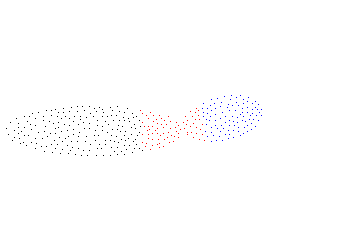
\includegraphics[width=.40\textwidth]{results/2_1parts_clusters_2th}} &
		\fbox{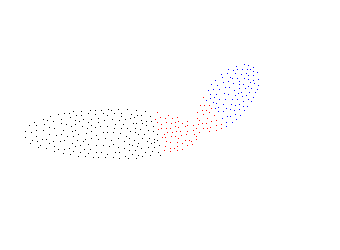
\includegraphics[width=.40\textwidth]{results/2_2parts_clusters_2th}} 
		\\
		(a) & (b)
		\\[4pt]	%vertical extra spacing (4 points)
		\fbox{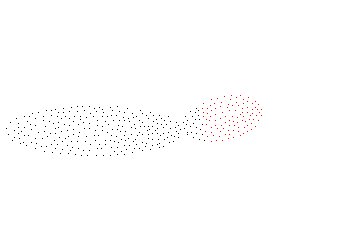
\includegraphics[width=.40\textwidth]{results/2_1parts_rigidParts_2th}} &
		\fbox{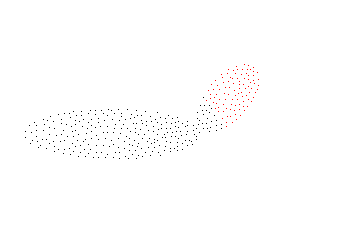
\includegraphics[width=.40\textwidth]{results/2_2parts_rigidParts_2th}} 
		\\
		(c) & (d)
	\end{tabular}
	\caption{Taking a Mesh $M$ in two poses with only two rigid parts as input, with a threshold $\tau = 5$, 3 clusters are detected in $C_1$~(a) and $C_2$~(b),
		which results in 2 rigid parts in $C_1$~(c) and $C_2$~(d).}
	\label{fig:2rigidParts}
\end{figure}
%%
\begin{figure}
	\centering\small
	\begin{tabular}{@{}c@{\hspace{2mm}}c@{}} % mittlerer Abstand = 12mm
		\fbox{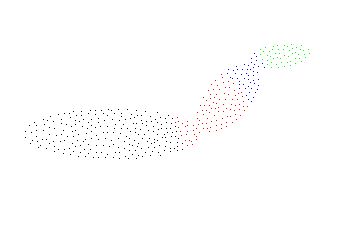
\includegraphics[width=.40\textwidth]{results/3_1parts_clusters_2th}} &
		\fbox{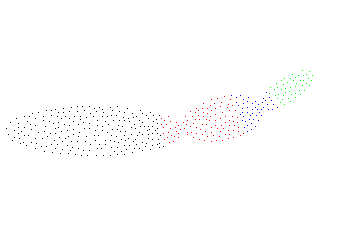
\includegraphics[width=.40\textwidth]{results/3_2parts_clusters_2th}} 
		\\
		(a) & (b)
		\\[4pt]	%vertical extra spacing (4 points)
		\fbox{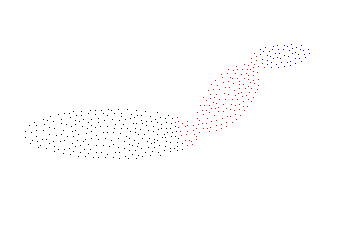
\includegraphics[width=.40\textwidth]{results/3_1parts_rigidParts_2th}} &
		\fbox{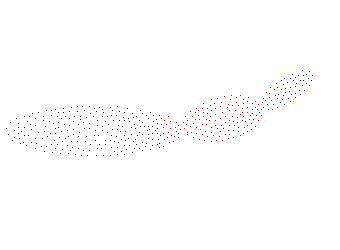
\includegraphics[width=.40\textwidth]{results/3_2parts_rigidParts_2th}} 
		\\
		(c) & (d)
	\end{tabular}
	\caption{Taking a Mesh $M$ in two poses with three rigid parts as an input, with a threshold $\tau = 6$, 4 clusters are detected in $C_1$~(a) and $C_2$~(b),
		which results in 3 rigid parts in $C_1$~(c) and $C_2$~(d).}
	\label{fig:3rigidParts}
\end{figure}
The segmentation into rigid parts is also apparent, when visualizing the point registration between $C_1$ and $C_2$ (see figure \ref{fig:ICPResults}). Two associated points from $C_1$ and $C_2$ are thereby linked with green lines. Comparing the registration results before and after a segmentation into rigid parts clearly shows, that the registration of rigid parts with the ICP results in a lower matching error $e$.
%%	
\begin{figure}[H]
	\centering\small
	\begin{tabular}{cc}
		\fbox{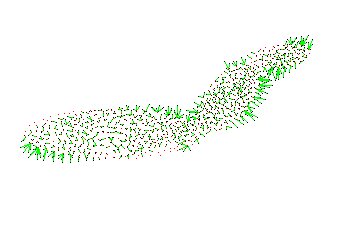
\includegraphics[width=0.45\textwidth]{results/non-rigid_3parts_associations}} &	
		\fbox{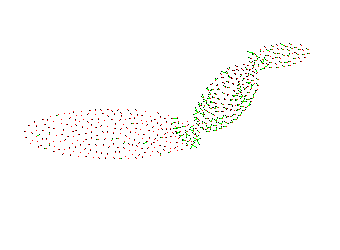
\includegraphics[width=0.45\textwidth]{results/rigid_3parts_associations}} 
		\\
		(a) & (b) 
	\end{tabular}
	\caption{Registration of $C_1$ and $C_2$ before the segmentation into rigid parts (a) and after the segmentation (b).} 
	\label{fig:ICPResults}
\end{figure}
%%		
In case of a more complex object, the simple segmentation algorithm fails. Although varying threshold $\tau$ for the matching, there are either too many or few rigid parts detected. When using $\tau = 7$ (see figure \ref{fig:4rigidPartsHighTH}) only 3 clusters and rigid parts can be detected. By decreasing $\tau$ to 6 (see Figure \ref{fig:4rigidParts}), further subdividing is done, which leads to a too high number of rigid parts and clusters.
%%
\begin{figure}[H]
	\centering\small
	\begin{tabular}{cc}
		\fbox{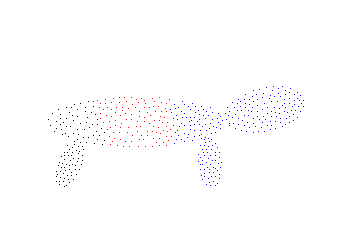
\includegraphics[width=0.45\textwidth]{results/4_1parts_clusters_rigidParts_7th}} &	
		\fbox{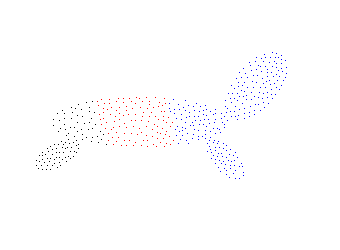
\includegraphics[width=0.45\textwidth]{results/4_2parts_clusters_rigidParts_7th}} 
		\\
		(a) & (b) 
	\end{tabular}
	\caption{Taking a more complex Mesh $M$ in two poses with four rigid parts as an input, with a threshold $\tau = 7$, 3 clusters and rigid parts can be detected in $C_1$~(a) and $C_2$~(b).} 
	\label{fig:4rigidPartsHighTH}
\end{figure}
\begin{figure}[H]
	\centering\small
	\begin{tabular}{@{}c@{\hspace{2mm}}c@{}} % mittlerer Abstand = 12mm
		\fbox{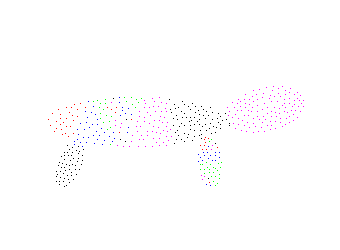
\includegraphics[width=.40\textwidth]{results/4_2parts_clusters_6th}} &
		\fbox{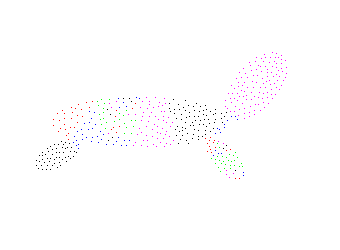
\includegraphics[width=.40\textwidth]{results/4_1parts_clusters_6th}} 
		\\
		(a) & (b)
		\\[4pt]	%vertical extra spacing (4 points)
		\fbox{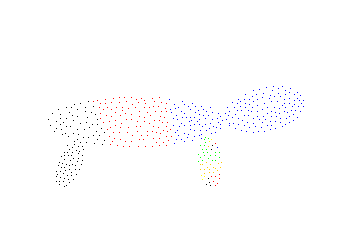
\includegraphics[width=.40\textwidth]{results/4_1parts_rigidParts_6th}} &
		\fbox{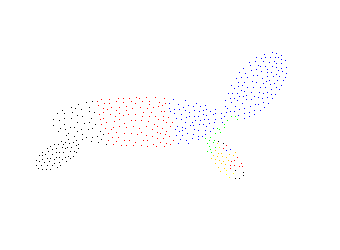
\includegraphics[width=.40\textwidth]{results/4_2parts_rigidParts_6th}} 
		\\
		(c) & (d)
	\end{tabular}
	\caption{Taking a more complex Mesh $M$ in two poses with four rigid parts as an input, with a threshold $\tau = 6$ , 35 clusters are detected in $C_1$~(a) and $C_2$~(b),
		which results in 26 rigid parts in $C_1$~(c) and $C_2$~(d).}
	\label{fig:4rigidParts}
\end{figure}	
The algorithm generally works for simple objects, in which the rigid parts are linked like a chain. Still, the segmentation location is not accurate, which might be disposed by introducing weights to points located near a joint. For more complex object with a skeleton structure, e.g. a human, where one rigid part is linked to more than two rigid parts, this simple implementation fails. In this case, another approach has to be found, as a skeleton structure is more complex to extract than a simple chain structure.

\section{Improvements}

In case of articulated objects with a skeleton structure, the segmentation algorithm in its simple form fails. The main reasons are the following:
%%
\begin{itemize}
	\item By recursively subdividing $C_1$ and $C_2$ the detected sub clusters might actually count to more than one and being located apart from each other. 
	\item In case of a matching cluster being a part of a rigid part, no further operations are done with the match. The rigid part is anticipated to be generated by merging neighboring sub clusters.
	\item By further sub dividing clusters, the merging becomes more difficult, as the clusters are scattered next to each other.
	\item The detection of joints is not exact although the segmentation in the approximate rigid parts succeeds as sub clusters are good enough to fit, but still there might be better fits with less or more points.
\end{itemize}
%%
Thus, the initial approach needs to be extended, which solved the issues being mentioned.

\subsection{Region growing}
During the segmentation of an object in two different poses, there is the general case that the divided parts being compared do not contain the same number of points. As this state might come to undesirable matching errors, parts with the same sizes could be generated by region growing. This can be e.g. implemented by starting with the most outside point of two poses and grow regions with the same size of points which are then compared. Furthermore, the detection of multiple clusters can be treated, in case of subdividing clusters. The detected clusters are as a result treated individually.

\subsection{Matching error}
Another improvement is the assurance that during the ICP procedure each point only has one nearest neighbor and also considering the case, that there are not always the same amount of points in two clusters (uneven number of points). By doing so, not all points would contribute to the matching error. Furthermore, weights should be added to the points, especially points located near a joint should be treated cautiously. A cluster could be therefore further subdivided, if a minimum number of points is above the error threshold $\tau$ and not the average. 

\subsection{Initial alignment of clusters}
The initial ``Divide and Conquer'' approach is used to detect two matching sub clusters of $C_1$ and $C_2$. But unlike previous implementations, the rigid parts are not detected by a following merging step, but by region growing, until the matching error $e$ is above the specified threshold $\tau$.
If a rigid part is detected, it is stored and the same procedures initiates with the other points of $C_1$ and $C_2$. By doing so, all rigid parts are sequentially detected from one direction to the other.

%\subsection{Error handling}
%The region growing procedure needs to terminate if points of another rigid part are added. Following, a higher matching error $e$ is detected. To guarantee successful rigid part detection this procedure premises that the regions in two comparing sub clusters grow the same way, otherwise the region growing might terminate before detecting the whole rigid part. 

\subsection{Segmentation of articulated objects}
The most crucial deficit  of the proposed algorithm is that is does not work with articulated objects, whose parts are not simple linked as a chain, but a rigid part can have more than two linking rigid parts. An example would be the skeleton of humans and most animals. As a result, the objects are simply too complex to linearly subdivide them. One improvement proposition is thereby the initial alignment of the object, that the largest rigid part is aligned.  A similar approach was taken during the LRP algorithm \cite{guo2016correspondence}. Then, recursively linked parts of this largest rigid part are detected (see section \ref{LRP}).

\subsection{ICP}
Sparse correspondences of two input clusters $C_i$ and $C_j$ were initially achieved by applying the Iterative closest point algorithm. Thereby, the two input clusters are aligned by means of the PCA. Following, corresponding points of $C_i$ and $C_j$ are only considered, if they are \textit{reciprocal} (see subsection \ref{functionalityLRP}). Furthermore, the euclidean distance between two cluster points $d(\boldsymbol{p}_i,\boldsymbol{p}_j)$ must be below a predefined threshold $\tau$. As a consequence, points being located far away from each other do not contribute to the alignment of $C_i$ and $C_j$ and are not stored as correspondence. Those are assumed to be small rigid parts with different transformations.

\subsection{Main drawbacks}
The main drawback of the algorithm represents the first initial alignment of the two poses of the articulated object. Thereby, it is directly dependent on the symmetry of the pose. The less symmetry the higher the changes that the initial alignment on the largest rigid part might fail. The reason is that the ICP expects a good starting alignment. As it is assumed that the major largest rigid part contributes most to the principal axis and the initial alignment, it would work. But in case of an unbalance of the linked parts, the alignment of the LRP might shift in a certain direction and it might not be detected during the ICP. As a result the whole algorithm fails. Furthermore, touching of rigid parts (e.g. the hand touches the leg) constitute difficulties as the region growing would not detect those as potential linked clusters. 

\chapter{Feature-based approach}
\label{cha:FeatureApproach}

To solve the main drawbacks of finding reliable point correspondences for an initial alignment of $C_1$ and $C_2$ the focus on the second approach lies on point features. They are introduced as they provide additional, meaningful information about a point $\boldsymbol{p}_i$ besides its coordinates. For this reason, point feature histograms, namely ``Fast point feature histograms'' (FPFH) \cite{FPFH} are computed for all points of $C_1$ and $C_2$. Basically, a histogram of a point $\boldsymbol{p}$ describes the curvature of a surface described by itself and its $k$ neighbors. By detecting similar point feature histograms between $C_1$ and $C_2$, referred to as feature matching, point correspondences are acquired. These are then used for an initial alignment of $C_1$ and $C_2$ that their largest rigid parts overlap. Proceeding from the largest rigid part, linked rigid parts can be detected. This approach is closely related to Guo et al \cite{guo2016correspondence}. 

\section{Fast point feature histograms}
\label{FPFH}
The ``Fast Point Feature histograms'' algorithm is an improved approach of the `'Persistent Point Feature Histogram for 3D Point Clouds'' \cite{PPFH} in terms of computation time. It focuses on computing a feature histogram for a point $\boldsymbol{p}$ by comparing its normal $\vec{n}$ to the normals of all $k$ neighbors. The choice of those point features are the following: 
%%
\begin{itemize}
	\item rotation- and scale-invariant
	\item easy comparison of feature histograms
	\item approval of approach
	\item straightforward adaption of different dimensions (2D and 3D)
\end{itemize}
%%
The data input for this algorithm is a list of $n$ unordered points $\boldsymbol{p}_1(x,y,z), \cdots, \boldsymbol{p}_n(x,y,z)$ only providing information about the points coordinates in 3D space. As a result, no surface is supplied for the computation of feature histograms. Therefore, in an initial step the point normals need to be computed (see subsection \ref{normal}).

\subsection{Normal estimation}
\label{normal}
As a first step, the normals of all unordered points from the input clusters $C_1$ and $C_2$ are estimated, following the approach of Hoppe et al \cite{normals}. The normal $\vec{n}$ of point $\boldsymbol{p}$ can be computed by taking all neighboring points $k$ within a radius $r$ of $\boldsymbol{p}$ into consideration. Subsequently, a least error fit straight line $X$ in the form $ax + by +c = 0$ to all selected points including $\boldsymbol{p_i}$ is computed by minimizing the squared distances from all points
%%
\begin{equation}
\begin{split}
dist^2(x_i, y_i) = (ax_i + by_i + c)^2
\\
e =   \displaystyle\sum_{i=1}^{k} dist^2(x_i, y_i)
\end{split}
\end{equation}
%%
to $X$. This is done by computing the unknown parameters $a, b$ of $X$ with the covariance matrix 
%%
\begin{equation}
\begin{pmatrix}
\overline{x^2} - \overline{x} \cdot \overline{x} & \overline{xy} -\overline{x} \cdot \overline{y}\\
\overline{xy} -\overline{y} \cdot \overline{x} & \overline{y^2} -\overline{y} \cdot \overline{y}
\end{pmatrix} \cdot \begin{pmatrix}
a \\
b
\end{pmatrix} = \lambda \cdot \begin{pmatrix}
a \\
b
\end{pmatrix}
\end{equation}
%%
resulting in two pairs of an eigenvalue and eigenvector $(n_1,\lambda_1)$ and $(n_2,\lambda_2)$. The normal of $\boldsymbol{p}$ is computed solving the linear equation for the normal vector $\vec{n_2}$ which is represented by $\lambda_2$. The procedure is conducted for all points from $C_1$ and $C_2$ (see figure \ref{fig:normalEstimation}). 
%%
\begin{figure}[H]
	\centering
	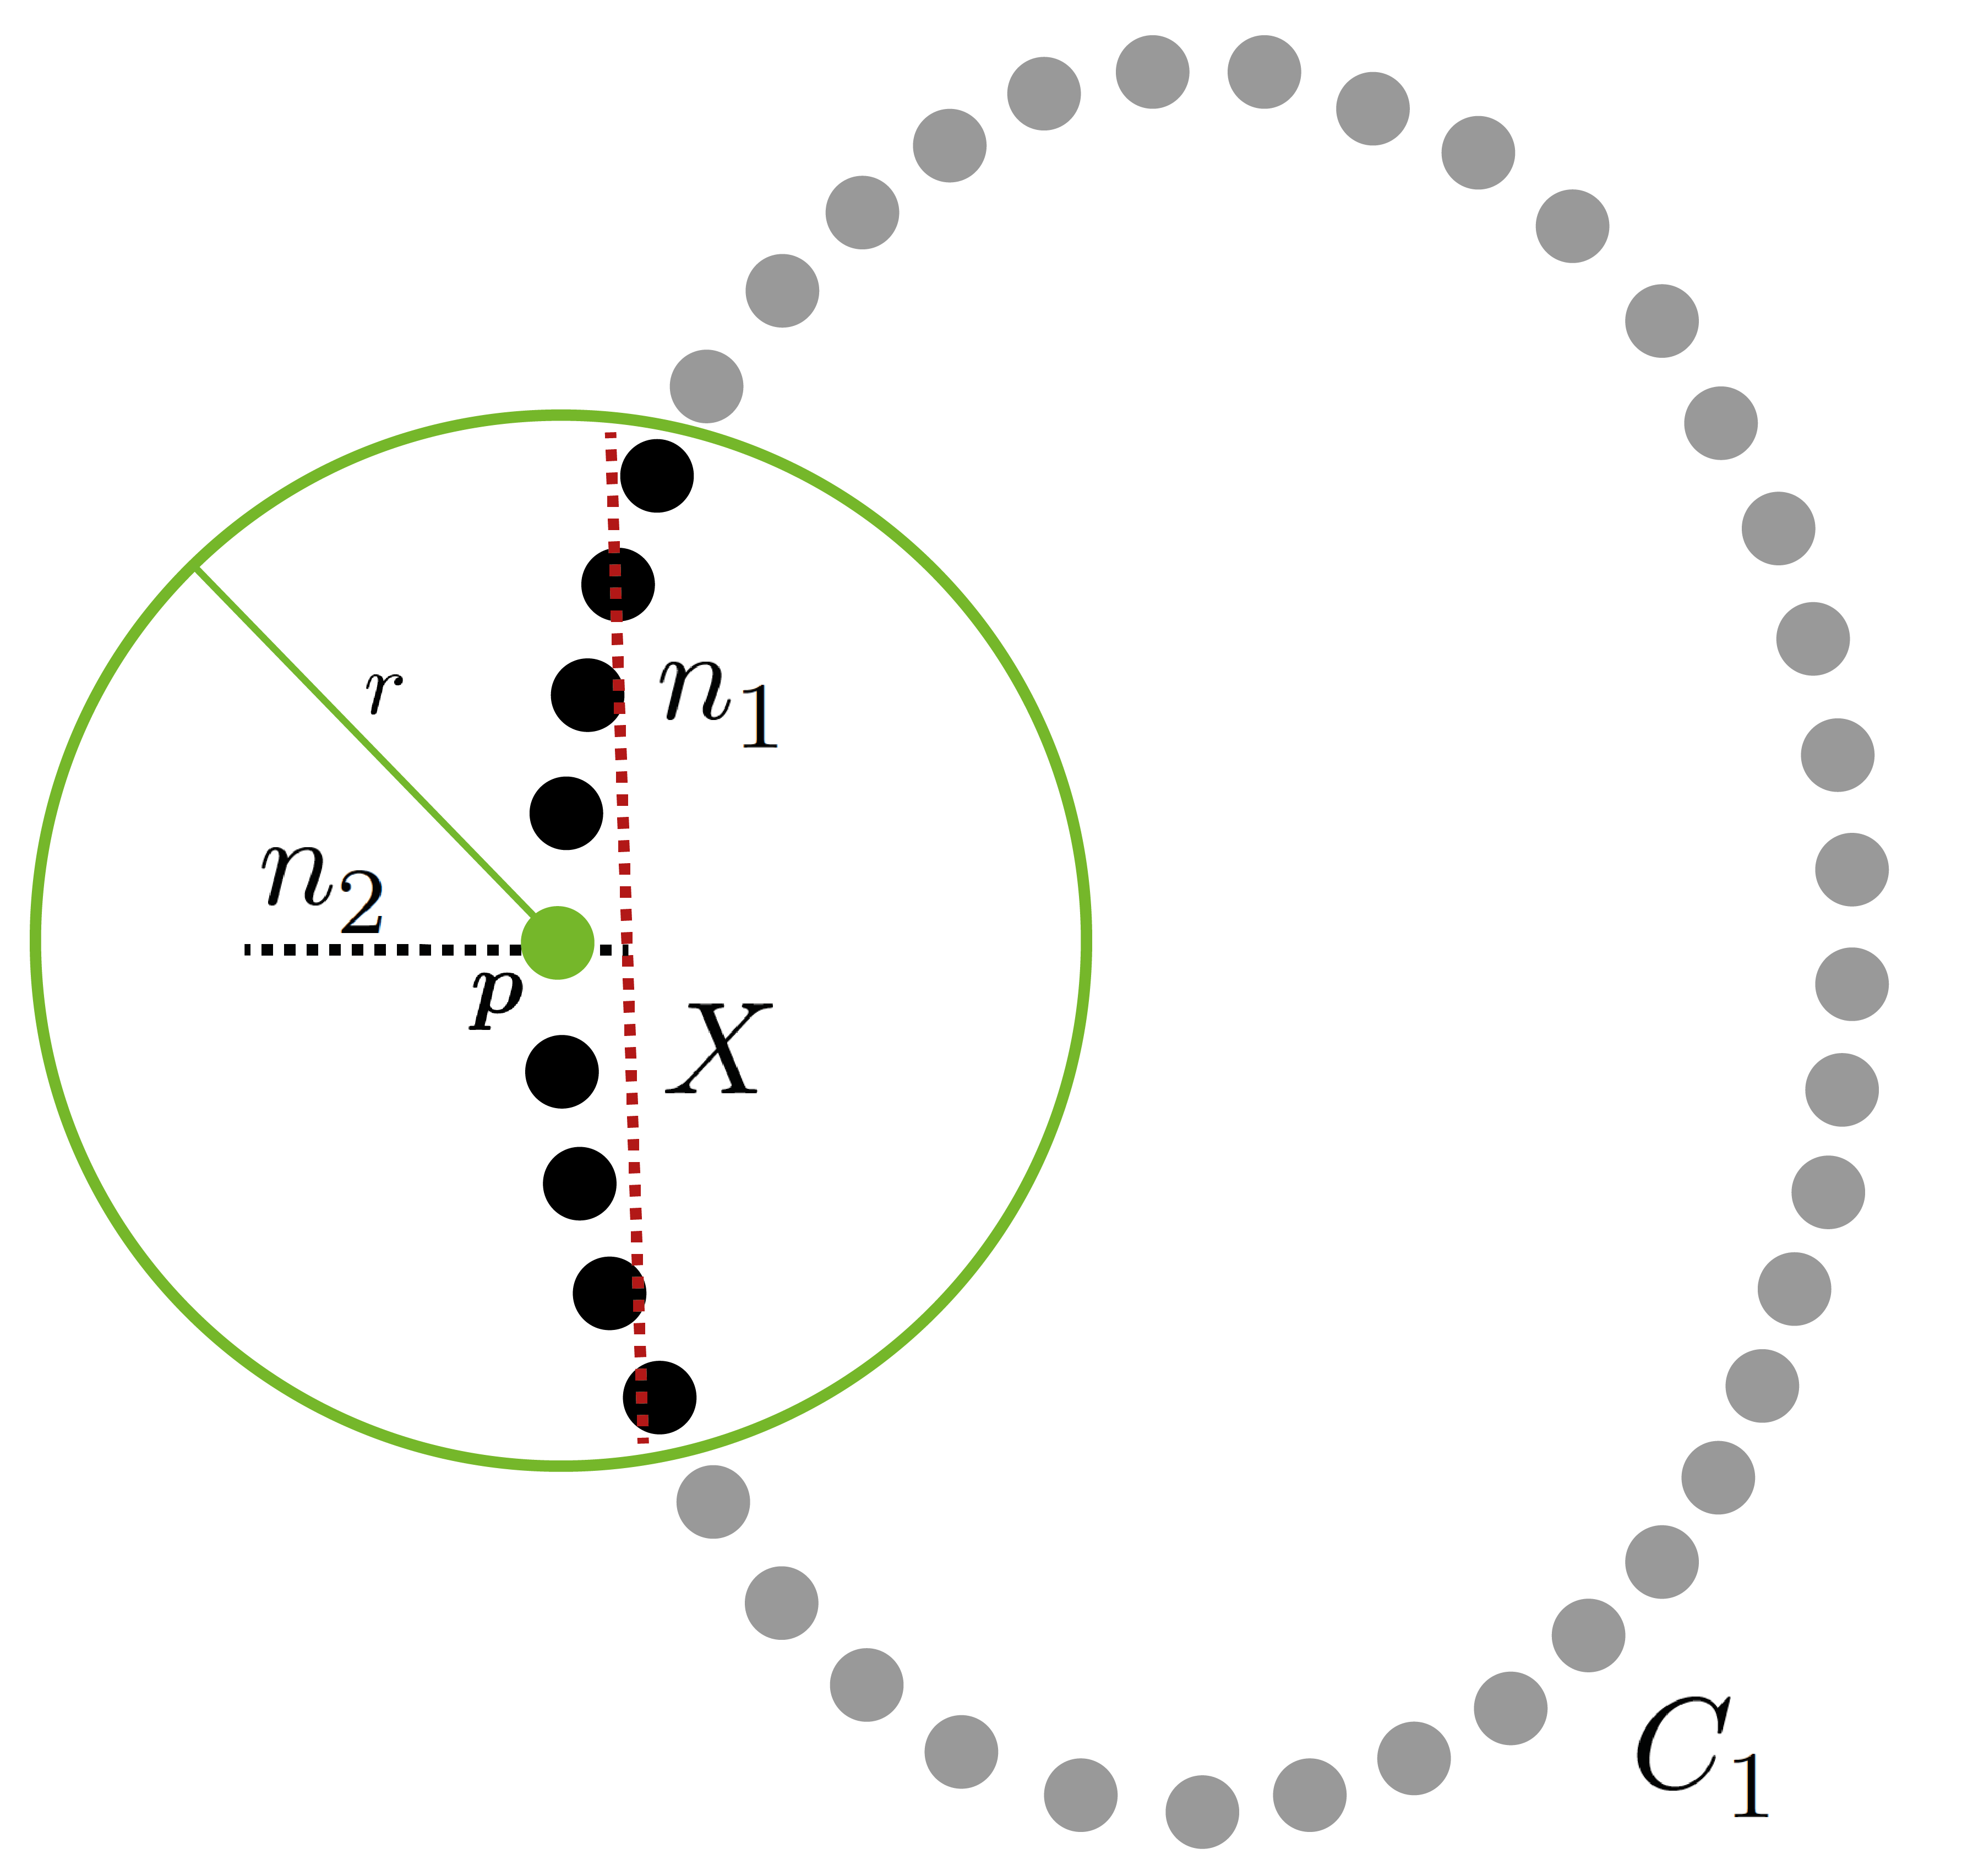
\includegraphics[width=0.4\linewidth]{normalEstimation}
	\caption{Normal estimation for a cluster point $\boldsymbol{p}$ of $C_i$ by a computation of the least squared fitting line $X$ of the neighborhood inside a radius $r$. Calculation of the eigenvectors $\vec{n_1}$ and $\vec{n_2}$ by forming the covariance matrix of  $\boldsymbol{p}_i$ and all $k$ points.}
	\label{fig:normalEstimation}
\end{figure}
%%
%TODO: fix image (C_i, ...)
%%
As a next step, it is required that all normals are equally oriented, as some might be flipped by 180°. Basically, all $n$ computed normals are traversed globally, starting with a normal $\vec{n}$ of a point $p$. Thereby, it is of particular importance to select a normal that assures consistent orientations between $C_1$ and $C_2$. Taking its orientation as parent normal $\vec{n_p}$, the angle $\delta$ between $\vec{n_p}$ and all neighboring normals $\vec{n_k}$ 
%%
\begin{equation}
\delta = \vec{n_p} \cdot \vec{n_k}, \quad \text{for $|\vec{n_p}|, |\vec{n_k}| = 1$}
\end{equation}
%%
is computed. In case of $\delta < 0$, $\vec{n_k}$ requires to be flipped 180° ($\vec{n_k} = -\vec{n_k})$. If all $k$ normals have been verified to be oriented in consideration of $\vec{n_p}$ any $\vec{n_k}$ is selected as current $\vec{n_p}$. The whole algorithm proceeds until all $n$ normals have been verified to correspond with their parent normal $n_p$ (see figure \ref{fig:flipping}).
%%
%TODO: add image normal flipping
%%
\begin{figure}[H]
	\centering\small
	\begin{tabular}{cc}
		\fbox{
\includegraphics[width=0.40\textwidth]{Placeholder}} &	
		\fbox{
\includegraphics[width=0.40\textwidth]{Placeholder}} 
		\\
		(a) & (b) 
	\end{tabular}
	\caption{Normal flipping of all normals computed on a cluster $C_i$ (a) to equally orient them (b).} 
	\label{fig:flipping}
\end{figure}
%%
\subsection{SPFH and FPFH}
As an intermediate step before computing the FPFH, the simplified point feature histogram (SPFH) of a point $\boldsymbol{p}$ is computed, which represents its relationship to its $k$ neighbors. This is achieved by calculating three geometric features between $\boldsymbol{p}$ and each of its $k$ neighbors $\boldsymbol{p_k}$. For further calculations, $\boldsymbol{p}_i$ represents the point having the smaller angle between its normal and the line connecting the point set, $\boldsymbol{p}_j$ corresponds to the other point. Using their normals $n_i$ and $n_j$ a Darboux $uvn$ frame $(u = n_i, v = (p_j - p_i) \times u, w = u \times v)$ is computed (see figure \ref{fig:darbouxFrame}). 

\begin{figure}[H]
	\centering
	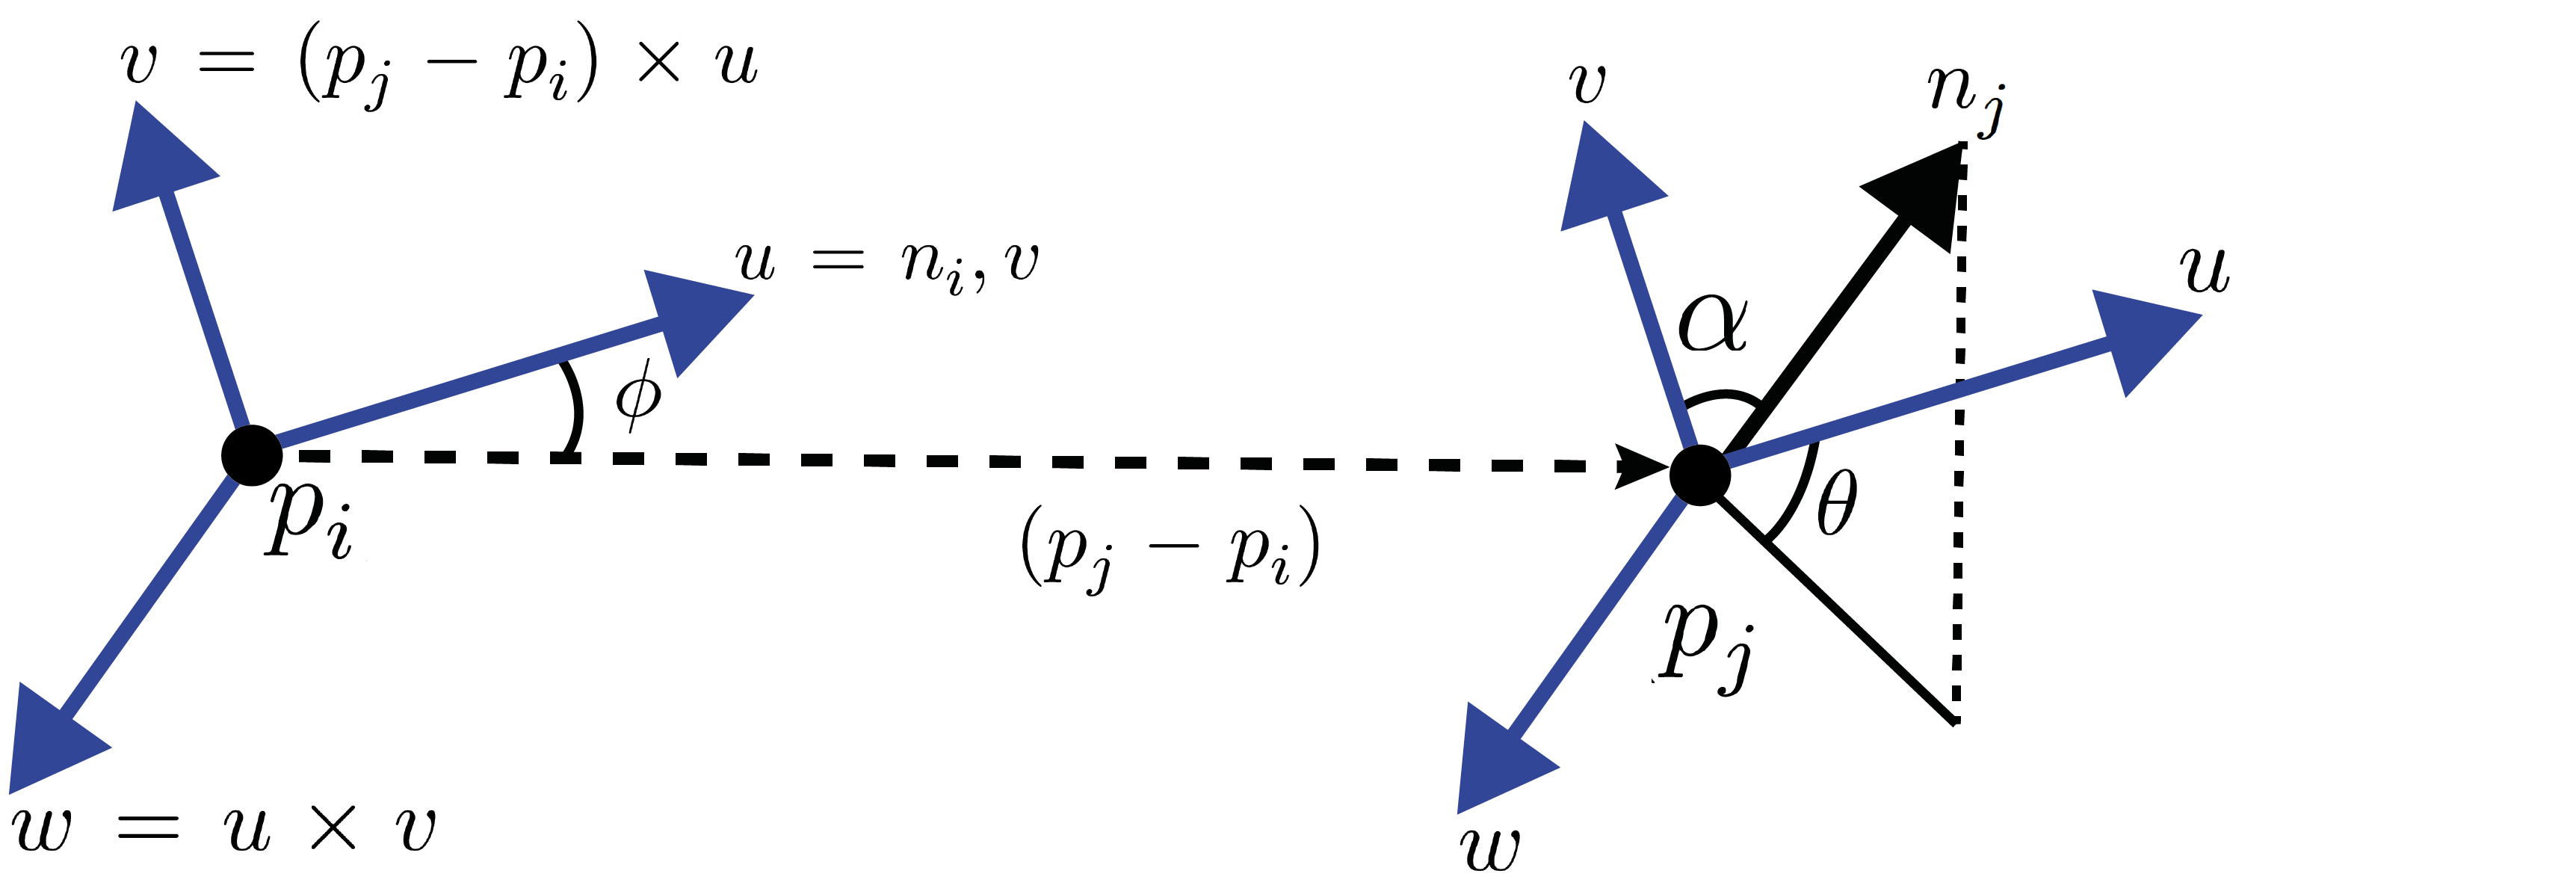
\includegraphics[width=0.8\linewidth]{DarbouxFrame}
	\caption{Computation of the Darboux frame $uvn$ in order to calculate the features between two point sets described by angles.}
	\label{fig:darbouxFrame}
\end{figure}

Consequently, the following angles
%%
\begin{equation}
\begin{split}
\alpha = v \cdot n_j
\\
\phi = (u \cdot (p_j - p_i))/\|p_j - p_j\|
\\
\theta = arctan(w \cdot n_j, u \cdot n_j)
\end{split}
\label{eq:AngularVariations}
\end{equation}
%%
are computed which are categorized into a histogram (see subsection \ref{histogram}). The SPFH of $\boldsymbol{p}$ is then weighted to its FPFH
%%
\begin{equation}
FPFH(\boldsymbol{p}) = SPFH(\boldsymbol{p}) + \frac{1}{n} \cdot \displaystyle\sum_{k=1}^{n}\frac{1}{w_k} \cdot SPFH(p_k)
\end{equation}
%%
by computing the SPFH for all of its $k$ neighbors. The weight $w_i$ represents the distance $d(\boldsymbol{p},\boldsymbol{p}_k)$. The influence region diagram for a Fast Point feature histogram of a query point $\boldsymbol{p_q}$ can be seen on Figure \ref{fig:FPFHregion}. 
%%
\begin{figure}[H]
	\centering
	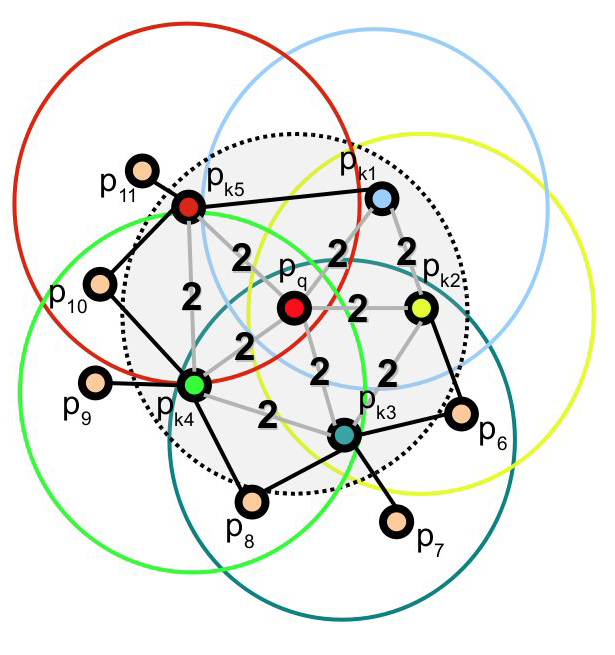
\includegraphics[width=0.4\linewidth]{FPFH_region}
	\caption{The point region for the calculation of the feature histogram for a query point $\boldsymbol{p}_q$. The SPFH of $\boldsymbol{p}_q$ and its neighbors (inside the grey circle) is weighted with the SPFHs of all $k$ neighbors (colored circles) \cite{FPFH}.}
	\label{fig:FPFHregion}
\end{figure}
%%
\subsection{Feature histograms}
\label{histogram}
The resulting feature values for each point $p$ of $C_1$ and $C_2$ in form of three angles between its neighbors $k$ are categorized using a histogram $H \{bin_1,\ldots,bin_b\}$ with $b = q^f$ bins to consider all possible combinations of the feature values. Thereby, $q$ represents the number of intervals the feature values should be categorized into. The number of feature values is represented by $f$, in this case three. Taking into account three feature values computed between a point set ($p$,$p_k$) the associated bin at the index $idx$
%%
\begin{equation}
idx = \displaystyle\sum_{i=1}^{i \leq f}q(f_i) \cdot 2^{i-1}
\end{equation}
%%
is incremented by 1. The function $q(f)$ returns the interval the feature is allocated to, ranging from 0 to $q - 1$. Finally, each bin contains the number of point pairs that are allocated in the specified value interval.As soon as the feature histograms of all points from $C_1$ and $C_2$ are computed only salient histograms are taken as comparison for point correspondence between $C_1$ and $C_2$ to reduce the correspondence space. In order to achieve that, the mean of all feature histograms $\mu$ of a cluster $C_i$ is computed. Subsequently, the distance of a feature histogram $H_i$ is compared to $H_\mu$ and in case of being outside the value $\mu \pm \sigma$ denoted as \textit{unique} and passed to the next step of detecting matching histograms between $C_1$ and $C_2$. The standard deviation
%%
\begin{equation}
\sigma = \frac{1}{N} \cdot \displaystyle\sum_{i=1}^{N}(H_i(b) - \overline{H_i})^2
\end{equation}
%%
is therefore calculated for all histograms $H_i$ with $N$ data entries of all cluster points. 
%%
\subsection{Feature matching}
\label{histogramCriteria}
As a next step, all \textit{unique} feature histograms of $C_1$ are aiming for detecting the most similar feature histogram from $C_2$. For that reason, different histogram-similarity criteria have to be determined to measure the similarity between two histograms $H_j$ and $H_k$ with each $b$ bins. In order to detect the best fitting histogram three main criteria most frequently applied in reference papers \cite{surfletPairRelation} \cite{localFeatureHistograms} are selected. As first criterion the squared euclidean distance (L2)
%%
\begin{equation}
\varepsilon(H_j, H_k) = \displaystyle\sum_{i=1}^{b}(H_j(i) - H_k(i))^2
\end{equation}
%%
is computed. In the reference paper of Guo et al. \cite{guo2016correspondence} the euclidean distance was selected as similarity criterion between feature histograms. It generally generates more point correspondences (see section \ref{ResultsLRP}) than the other two criteria. Furthermore, the statistical Chi-Square ($\chi^2$) divergence
%%
\begin{equation}
\chi^2(H_j, H_k) = \displaystyle\sum_{i=1}^{b}\frac{(H_j(i) - H_k(i))^2}{(H_j(i) + H_k(i))}
\end{equation}
%%
is examined which achieves less point correspondences than the L2 form but with a higher success rate. Finally, the Kullback-Leibler (KL) divergence
%%
\begin{equation}
\kappa(H_j, H_k) = \displaystyle\sum_{i=1}^{b}(H_j(i) - H_k(i)) \cdot ln \frac{H_j(i)}{H_k(i)}
\end{equation}
%%
is calculated, which is the most computational expensive one due to the application of $ln$. As a histogram with $q^f$ bins might contain a lot of zero values, in case of a division or logarithm all zero-values are replaced by the value 1.

\subsection{Adaptions for 2D}
\label{adaptions}
In order to compute the proposed feature histograms for 2D points, these need be treated like 3D points. This is achieved by setting each z-coordinate to 0 to allow all calculations originally targeting 3D points. 
2D point clouds are generally composed of less points than 3D point cloud, which results in less neighbor points for normal estimation and feature computation. As a result the computation time can be considerable reduced. 
As also the number of point correspondences are considerable reduced, all histograms are considered during the feature histogram matching, not only salient ones. 

\section{LRP algorithm}
\label{LRP}
The approach from Guo et al \cite{guo2016correspondence} aims to detect the largest rigid part (LRP) of two poses of an object to have a solid basis for a successful segmentation into the rigid parts. A similar procedure is aspired after in the proposed feature-based approach.

\subsection{Basic functionality}
\label{functionalityLRP}
As an initial step, the LRP algorithm attempts to detect the most reliable correspondences between two clusters $C_1$ and $C_2$. For that, local point descriptors (see section \ref{FPFH}) are computed. The requirement for a sparse correspondence between two cluster points $\boldsymbol{p}_i(x,y)$ and $\boldsymbol{p}_j(x,y)$ is that they are \textit{reciprocal}, which means that the according point feature histograms are the most similar from each other. Some of the sparse correspondences are assumed to be wrong. Therefore, RANSAC is applied on the point correspondences to aim for a single rigid transformation to detect the so-called ``largest rigid part'' (LRP), which is supported by the largest corresponding point cluster between $C_1$ and $C_2$. In case of a human, this would be the torso. Subsequently, all linked rigid parts to the LRP are detected by recursively applying the algorithm on grown clusters from the current LRP.

\subsection{Input data}
For the proposed 2D implementation, the 2D hulls of an articulated object in two different poses are taken as input (see Figure \ref{fig:inputPoses}). To support the point cohesiveness of a rigid parts after a transformation or segmentation joint-likely spheres were placed between rigid parts which are also used as rotation points. For the computation, those are treated to belong to a rigid part and no information about a joint are extracted. To achieve an indicator for the adjustment of thresholds (e.g. maximum distance to closest point), the resolution of the input clusters is computed. By applying the approach from \ref{clustering} the estimated resolutions accounts to 7.24 for $C_1$ and 7.56 for $C_2$.
%%
\begin{figure}[H]
	\centering\small
	\begin{tabular}{cc}
		\fbox{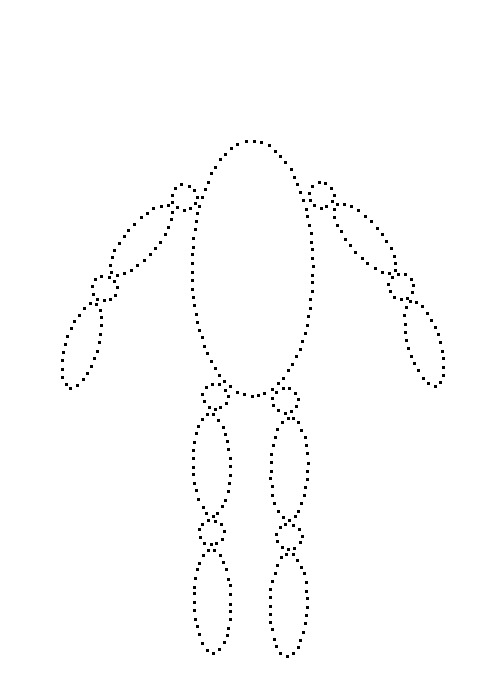
\includegraphics[width=0.40\textwidth]{InputPose1}} &	
		\fbox{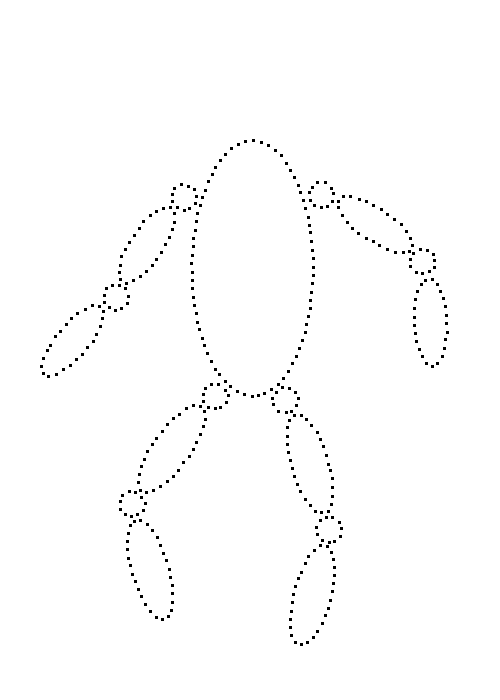
\includegraphics[width=0.40\textwidth]{InputPose2}} 
		\\
		(a) & (b) 
	\end{tabular}
	\caption{Taking an articulated object (puppet) in two different poses $C_1$ (a) and $C_2$ (b) in form of a 2D point cloud representing its hull as input.} 
	\label{fig:inputPoses}
\end{figure}
%%
\subsection{Implementation steps}
In order to re-implement the algorithm in 2D, only minor modifications concerning point coordinates and feature histograms had to be accomplished (see subsection \ref{adaptions}). The most crucial part of the whole algorithm is the initial alignment of $C_1$ and $C_2$ in order to detect the actual largest rigid part of the articulated object. This step is of particular importance, as the subsequent detection of further rigid parts proceeds from there. Concerning the detection of linked rigid parts, an approach with less computation steps and time was implemented. Generally, the implementation can be split into main parts.
\begin{enumerate}
	\item The PCA is employed on the input clusters $C_1$ and $C_2$ to estimate the normals of all points.
	\item Point feature histograms (FPFH) are computed for all points of $C_1$ and $C_2$. Sparse point correspondences are computed by feature matching. A point correspondence needs to be \textit{reciprocal}.
	\item The RANSAC approach is applied on these correspondences to detect a transformation $T$ that aligns $C_1$ and $C_2$. In each iteration, clusters are detected from overlapping points. The LRP is assigned to the resulting biggest point cluster.
	\item Unmatched clusters from $C_1$ and $C_2$ are taken as input to detect linked rigid parts from the LRP, which is achieved by region growing.
	\item Joints are estimated between the current LRP an all detected clusters linked to the LRP. Those are considered for allocating corresponding rigid parts of $C_1$ and $C_2$.
	\item Linked rigid parts are detected by rotating a cluster around its joint and finding the largest overlapping cluster. Certain constraints and a weighted error are taken into account.
\end{enumerate}

\subsection{Detection of sparse correspondences}
\label{correspondences}
As a first, the normals as well as the feature histograms for all points of $C_1$ and $C_2$ (see section \ref{FPFH}) are computed. Results of the normal flipping procedure can be seen on figure \ref{fig:normalFlipping}.

%TODO: Picture of normal flipping
\begin{figure}[H]
	\centering\small
	\begin{tabular}{cccc}
		\fbox{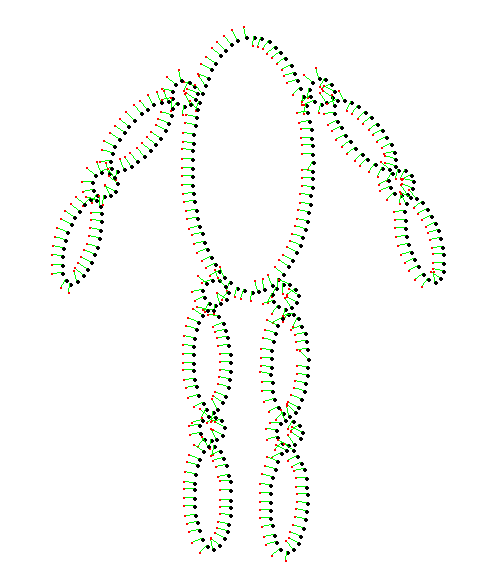
\includegraphics[width=0.23\textwidth]{Normals_C1_cropped}} &	
		\fbox{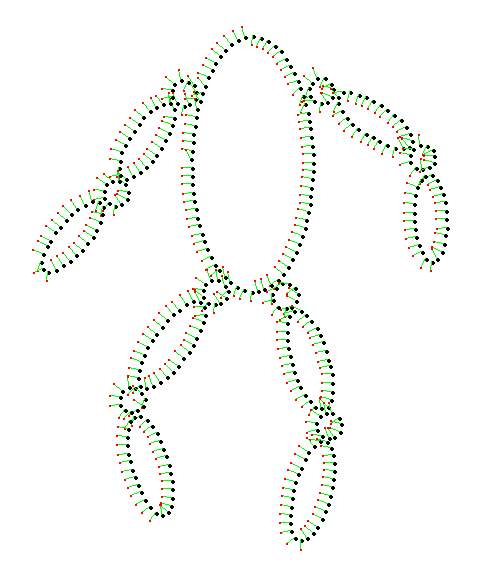
\includegraphics[width=0.23\textwidth]{Normals_C2_cropped}} &	
		\fbox{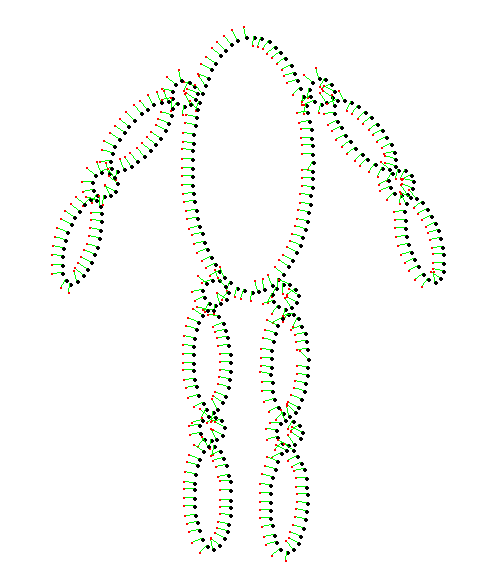
\includegraphics[width=0.23\textwidth]{Normals_C1_cropped}} &	
		\fbox{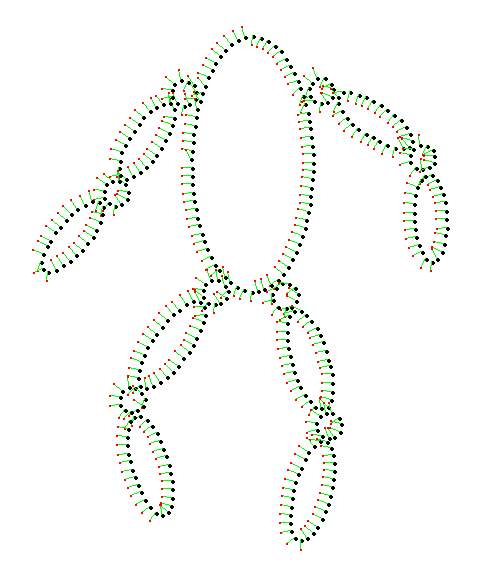
\includegraphics[width=0.23\textwidth]{Normals_C2_cropped}} 
		\\
		(a) & (b) & (c) & (d)
	\end{tabular}
	\caption{Normal estimation of two Cluster $C_1$ and $C_2$ (a) and (b) a subsequent global traversing of all normals to orient them similar (c) and (d).} 
	\label{fig:normalFlipping}
\end{figure}
It can be observed that the flipping of normals does not globally succeed. The causes are corner positions of the 2D hull. Considering two normals surrounding a corner point, the normals are expected to face each other. But during the normal flipping they are similarly oriented, although the corner point between them should counteract this behavior. For this reason the global flipping of the normals, considering the given data set, leads to a high number of false point correspondences. A possible solution would be the introduction of more points, especially forming a corner.
%%
%TODO: test with new dataset
%%
For the detection of sparse correspondences between $C_1$ and $C_2$ three histogram distances (see section \ref{histogramCriteria}) are taken into account. Depending on the chosen distance as criteria, more or less correspondences can be detected, refer to section \ref{ResultsLRP} for a detailed comparison. The mean histogram of all histograms as well as a \textit{unique} histogram can be seen on \ref{fig:meanHistogram}. 
%%
%TODO: Picture of mean histogram + similar histogram
%%
\begin{figure}[H]
	\centering\small
	\begin{tabular}{cc}
		\fbox{
\includegraphics[width=0.45\textwidth]{Placeholder}} &	
		\fbox{
\includegraphics[width=0.45\textwidth]{Placeholder}} 
		\\
		(a) & (b) 
	\end{tabular}
	\caption{Computing the $\mu$ histogram of $C_1$ to represent frequently arising feature histograms (a). A \textit{unique}  histogram is stated by considerably deviating from the $\mu$ histogram (b).} 
	\label{fig:meanHistogram}
\end{figure}
Figure \ref{fig:sparseCorrespondences} represents the point correspondences between $C_1$ and $C_2$ resulting from feature matching. It is clearly evident that points located near a corner are more likely to detect a reciprocal point correspondence than points located at smooth surfaces. The reason is, that those features are determined as \textit{unique} which makes them more distinguishable. On the contrary, all points located on a smooth surface have similar feature histograms.
%%
\begin{figure}[H]
	\centering \small
	\begin{tabular}{c}
		\fbox{\includegraphics[width=0.80\textwidth]{featureCorrespondences_chiSquare}} 
	\end{tabular}
	\caption{Visualization of the point correspondences established from most similar, reciprocal feature histograms using the chi-square distance between all points of $C_1$ (red) and $C_2$ (blue).}
	\label{fig:sparseCorrespondences}
\end{figure}
%%
As some of those correspondences are assumed to be wrong, a RANSAC approach is applied on all correspondences to reject false ones (see subsection \ref{detectionLRP}).
%%
\subsection{Detection of the largest rigid part}
\label{detectionLRP}
The dense point correspondences from the previous computation step (see subsection \ref{correspondences}) may contain several errors. Therefore, RANSAC is applied as a next step to detect a single rigid transformation $T$ that leads to the biggest overlapping point cluster of $C_i$ and $C_j$. Thereby, in each iteration, 2 random correspondences are selected and used for the calculation of $T$ which is applied on $C_i$ to be translated on $C_j$. 
%%
%TODO: Show Matrices of the RANSAC
%%
The number of required iterations for a successful alignment highly depends on the ratio of right and wrong point correspondences. This ration is determined by visual assessments, in case of the chi-square distance approximately 20\% of the point correspondences are assumed to be correct. By calculating the probability that almost assures (99\%) a write alignment
%%
\begin{equation}
\begin{split}
1 - (n \cdot q^n) = 0.99\\
1 - (n \cdot 0.8^n) = 0.99\\
n = 247.857
\end{split}
\end{equation}
%%
the number of iterations is set to 250.
%%
In each iteration, clusters are grown from all overlapping points with an euclidean distance $d(\boldsymbol{p}_i,\boldsymbol{p}_j)$ again below a predefined threshold $\tau$. The procedure is applied both on $C_i$ and $C_j$ which results in two rigid parts as output representing the largest detected clusters (see figure \ref{RANSAC}).
%%
\begin{figure}[H]
	\centering\small
	\begin{tabular}{cc}
		\fbox{\includegraphics[width=0.40\textwidth]{RANSAC_1000_chiSquare_ref}} &	
		\fbox{\includegraphics[width=0.40\textwidth]{RANSAC_1000_chiSquare_target}} 
		\\
		(a) & (b) 
	\end{tabular}
	\caption{Computation of the largest rigid part from $C_1$ (a) and $C_2$ (b) by applying RANSAC on the detected point correspondences.} 
	\label{fig:RANSAC}
\end{figure}
%%
The final transformation $T$ of the RANSAC approach, which leads to the largest overlapping clusters, is applied on the reference cluster. This procedure is required in order to similarly align $C_1$ and $C_2$ for further computations (see subsection \ref{CorrespondingClusters}).

\subsection{Cluster detection by region growing}
\label{cluster}
After successfully detecting a ``largest rigid part'' $P_i$ and $P_j$ for each input clusters $C_i$ and $C_j$ they are added to a list of rigid parts $\mathcal{P}$. Potential linked rigid parts are detected from region growing of all unclustered points $\mathcal{U} =  \{\boldsymbol{u}_1,\ldots,\boldsymbol{u}_n\}$. Those comprise all cluster points of $C_1$ and $C_2$ excluding already detected largest rigid parts $\mathcal{P}$. An adapted region growing procedure from subsection \ref{RegionGrowing} is applied with the previously detected LRP as seed. 
For this approach, it does not only return the largest cluster, but all clusters above a certain size. The result is a set of clusters $\mathcal{C}$ for each $C_i$ and $C_j$. As a next step, a preliminary joint $\boldsymbol{j}$ is estimated for each output clusters. This is achieved by detecting the closest points between $P_i$ and one of its clusters $C_i$. The joints are required for the detection of corresponding cluster between $C_1$ and $C_2$ (see subsection \ref{CorrespondingClusters}). Furthermore, there are used as joint weights for the detection of linked rigid parts (see subsection  and \ref{JointWeights}).

\subsubsection{Establishment of corresponding clusters}
\label{CorrespondingClusters}
In case of detecting more than one cluster resulting from region growing from each $P_1$ and $P_2$ it must be verified which clusters correspond to each other. This might be for example the case for the extremities linked to the torso. This association step is essential, as the detection of linked parts to the previously detected LRP assumes two clusters representing the same set of rigid parts. Thereby, the provisional joints $\mathcal{J}$ estimated for all clusters are used to associate two clusters of $C_1$ and $C_2$. Thereby the clusters with reciprocal closest joints, represented by the euclidean distance $d(\boldsymbol{j}_i,\boldsymbol{j}_j)$, are assumed as associated clusters.

\subsection{Detection of linked rigid parts}
\label{JointWeights}
In the reference paper the feature matching in combination with RANSAC for detecting point correspondences was reapplied on the linked clusters to the already detected rigid parts. However, this approach is not successful in the current 2D application. The reason is that the point features are not meaningful due to the reduced number of points and similarity of shapes. In order to iteratively detect further rigid parts linked to already detected ones another approach is developed which manages to operate less computational-expensive and less time-consuming as RANSAC and feature computation is not required. Thereby, the knowledge is used that rigid parts are transformed by rotating around a joint. For that purpose, the estimated joints $\mathcal{J} = j_1,\cdots,j_n$ resulting from the approach of subsection \ref{cluster} are taken into account. As a first step, two input clusters $C_i$ and $C_j$ are transformed that their joints overlap. Next, the primary axis of $C_i$ and $C_j$ are aligned to guess an initial alignment which should further reduce the computation steps. Then, $C_i$ is iteratively rotated around its joint into the direction of an decreasing least squares error $e$ in order to overlap with $C_j$. By iteratively updating $e$ after each rotation step, a best overlapping position between the linked rigid parts can be detected. Thereby, the preliminary joints are used as weights. A point $p_i$ being located far away from its allocated joint $J_n$ does not contribute as much to the matching error as points located near the joint. A weight $w$ is calculated by comparing the distance $d(p_i, J_n)$ to the maximal distance $d_{max}$ between $J_n$ and the farthermost allocated point. Subsequently a total matching error $e$
%
\begin{equation}
\begin{split}
w_i = \| \boldsymbol{p}_i - \boldsymbol{j}_n\| \cdot \frac{1}{d_{max}}
\\
e = \displaystyle\sum_{i=1}^{m}\| \boldsymbol{p}_i - \boldsymbol{q}_i\|^2 \cdot (1 - {w_i})^2
\end{split}
\label{eq:jointWeightError}
\end{equation}
%
is achieved by combining the distance of a point to its closest point and the joint weight $w$. The error is squared in order to further weaken the influence of cluster points being located far away from the joint. The final detected rigid parts are represented by the biggest cluster resulting from a rotation with the lowest error $e$. As a last step, all points with a closest point below a certain threshold $\tau$ are taken as input for region growing. It is assumed, that two linked rigid parts are quite similar aligned, therefore the distance threshold $\tau$ is considerable small. The largest cluster is finally returned as detected linked part.
%%
\begin{figure}[H]
	\centering\small
	\begin{tabular}{ccc}
		\fbox{\includegraphics[width=0.30\textwidth]{LegRotation_Before_cropped}} &	
		\fbox{\includegraphics[width=0.30\textwidth]{LegRotation_After_cropped}}  &	
		\fbox{\includegraphics[width=0.30\textwidth]{LegRotation_Results_cropped}} 
		\\
		(a) & (b) & (c)
	\end{tabular}
	\caption{The joints $J_i$ and $J_j$ (green dots) of the reference cluster $C_i$ (red) and the target cluster $C_j$ (blue) are overlapped. The closest points for $C_i$ are computed (a). Stepwise rotation of $C_i$ onto $C_j$ in the direction of a decreasing error until $e$ does not further decrease (b). Final overlapping clusters from taking all closest points of $C_i$ and $C_j$ below a distance threshold $\tau$ (c).} 
	\label{fig:jointRotation}
\end{figure}
%%
With varying distance thresholds $\tau$ for the selection of closest points or region growing, actual target points may be skipped or unnecessary points from another rigid part are added. Those circumstances lead to difficulties for the detection of linked parts. Detailed results about this appearance is discussed in section \ref{ResultsLRP}.

\section{Implementation}
\label{ImplementationLRP}
For the implementation in Java the individual steps of the largest rigid part algorithm have been split into individual classes for a better overview. Again ImageJ was used as processing library.
%
%TODO: Add class graph of implementation
%
\subsection{Iterative Segmentation}
The whole algorithm initiates from the \texttt{Segmentation} class, where all steps proposed in section \ref{LRP} are implemented (see algorithm \ref{alg:segmentation}). Basically, the segmentation proceeds until no unclustered points from $C_1$ and $C_2$ are remaining. As a first step of the iterative segmentation approach already detected rigid parts are removed from the unclustered points (\texttt{removeAllLRPs()}). As a next step, clusters are detected either for an initial input or in case of an already detected LRP, to detect its the linked parts. Joints are only estimated in case of a previously detected rigid part which is the case for all iterations except the first one. Then, all matching clusters are added to a \texttt{Stack} (\texttt{pushMatchingClusters()}) to be processed in form of a ``last in - first out'' procedure. In case of an empty stack, all clusters have been processed and the algorithm terminates. 

\begin{lstlisting}
while (unclusteredReference.size() > MIN_SIZE || !clusters.isEmpty()) {

	removeAllLRPs();

	referenceClusters = RegionGrowing.detectClusters(unclusteredReference);
	targetClusters = RegionGrowing.detectClusters(unclusteredTarget);

	if (currentLrps != null) {
		detectJoints(currentLrps, referenceClusters, targetClusters);
	}

	if (referenceClusters.size() != 0 && targetClusters.size() != 0) {
		pushMatchingClusters();
	}

	if (clusters.isEmpty()) {
		return;
	}
...
}
\end{lstlisting}

If there are still clusters existent, two matching ones are popped from the Stack. If the clusters do not own an allocated joint, no LRP has been detected yet. Therefore, the \texttt{FeatureMatching} class (see subsection \ref{FeatureMatching}) is applied on the matching clusters. In combination with RANSAC a largest rigid part can be detected. On the other hand two LRPs can be detected by rotation two clusters around their joints. In this case the \texttt{PartDetection} class is taken advantage of to detect a linked rigid part to the previously detected LRP.

\begin{lstlisting}
while (unclusteredReference.size() > MIN_SIZE || !clusters.isEmpty()) {
...
	currentClusters = clusters.pop();

	if (currentClusters[0].getJoint() == null) {
		FeatureMatching fm = new FeatureMatching(currentClusters[0], currentClusters[1]);
		Map<Integer, Integer> denseCorrespondances = fm.getCorrespondences();

		if (denseCorrespondances.size() < 3) {
		return;
		}

		RANSAC ransac = new RANSAC(currentClusters[0], currentClusters[1], denseCorrespondances);
		currentLrps = ransac.getLargestRigidParts();
		unclusteredReference = ransac.getTransformedReferencePoints();
	}

	else {
		PartDetection pd = new PartDetection(currentClusters[0], currentClusters[1]);
		currentLrps = pd.getLinkedParts();
	}

	if (currentLrps[0].getPoints().size() < 5) {
	} else {
	largestRigidParts.add(currentLrps);
	}
}
\end{lstlisting}
%%
%TODO: Write algorithm for Segmentation
%%
\begin{algorithm}[tbp]
	\caption{Computation of the normal and subsequently feature histograms of a cluster point $p_i$ with its $k$ neighbors inside a radius $r$. The fast point feature histograms FPFH are computed by weighting the SPFH of a $p_i$ and its $k$ neighbors.}
	
	\begin{algorithmic}[1]     % [1] = all lines are numbered
		\label{alg:segmentation}
		
		\Procedure{FPFH}{$p_i$} 
		\State $\mathit{C_{max}} \gets ()$
		\State $\mathit{C_{current}} \gets ()$
		\State $n \gets \mathit{sizeOf}(M)$
		\State $m \gets \mathit{sizeOf}(C_{current})$
		
		\While {$n$ > 0}
		\State $\mathit{c_{current}} \gets \mathit{c_{current}} + \boldsymbol{u}_1$
		\For{$i = 1,\ldots,m$}
		\State $M \gets M - C_{current}$
		\For{$j = 1,\ldots,n$}
		\If {\Call{$d$}{$\boldsymbol{p}_i, \boldsymbol{u}_j}< \tau$}
		\State $C_{current} \gets C_{current} + \boldsymbol{u}_j$
		\EndIf
		\EndFor
		\EndFor
		\State $M \gets M - C_{current}$
		\If{$m > \mathit{sizeOf}(C_{max})$}
		\State $C_{max} \gets C_{current}$
		\EndIf
		\State $C_{current} \gets ()$
		\EndWhile
		\State\Return $C_{max}$
		\EndProcedure	
	\end{algorithmic}
\end{algorithm}

\subsection{Feature Matching}
\label{FeatureMatching}
For the computation of normals, required for the computation of feature histograms, the class \texttt{NormalEstimation} is developed. It takes a point $p_i$ with its $m$ neighbors as input. Then, the least fitting error line on those input points is detected (as described in section \ref{correspondences}) and the smallest lambda value $\lambda_2$ selected as eigenvalue. By setting the x-value of the normal to 1.0, the y-value can be calculated with the eigenvalue $\lambda_2$. The resulting vector represents the normal vector $\vec{n}$ for $p_i$. In case of being exactly vertically or horizontally, the resulting value for y is either $infinite$ or $NaN$. In these cases the normal is either set to (0,1) or (1,0). As a last step, the normal is normalized.
%%
\begin{lstlisting}
double eigenvalue = Math.min(lambda1, lambda2);

	covarianceMatrix = new double[][] { 
		{ a - eigenvalue, b},
		{ b, c - eigenvalue}
	};

	double[] normal = new double[2];

	normal[0] = 1.0;
	normal[1] = (eigenvalue * normal[0] - covarianceMatrix[0][0] * normal[0])/covarianceMatrix[0][1];

	if(Double.isInfinite(normal[1])){
		normal[0] = 0;
		normal[1] = 1;
	} else if (Double.isNaN(normal[1])){
		normal[1] = 0;
	}

double length = Math.sqrt(Math.pow(normal[0], 2) + Math.pow(normal[1], 2));
normal[0] /= length;
normal[1] /= length;

point.setNormal(normal);
\end{lstlisting}
%%
A \texttt{ClusterPoint} class was implemented to store the normal $n_i$ for each point and the resulting feature histogram (FPFH) in form of a \texttt{Histogram} object containing an \texttt{int[]} array. For the calculation of a feature histogram of a point $p_i$, its $k$ neighbors are taken into account. The \texttt{FPFH} class implements various operations for vectors, like a dot or cross product to implement the formula from subsection \ref{FPFH}.
%%
\begin{lstlisting}
public void featureHistogram(p_i) {
	SPFH = SPFH(p_i);

	for (ClusterPoint p_k : p_i.getNeighborhood()) {
		double weight = p_i.distance(p_k);
		weightedSPFH = weightedSPFH.addHistograms(SPFH(p_k).multiplyHistograms(1.0 / weight));
	}
	
	FPFH = SPFH.addHistograms(weightedSPFH.multiplyHistograms(1.0 / p_i.getNeighborhood().size()));
	
	p_i.setFPFH(FPFH);
}
\end{lstlisting}

%TODO implementation of FPFH (index)

The feature histogram is computed by calculating the SPFH of a point by calculating angles between all its neighbors.




The combination of those three angles leads to an index in the histogram to be incremented. 





%%
Subsequently, point correspondences are detected by computing the distances between all feature histograms of $C_1$ and $C_2$ (see section \ref{correspondences}). For that, the closest point algorithm is configured to use the distance between histograms instead of the euclidean distance of point locations. Reciprocal point correspondences between $C_1$ and $C_2$ are returned in form of point indices \texttt{Map<Integer,Integer>}  of the clusters cluster points.
%%
%TODO: show chi-square distance
%%
\begin{lstlisting}
for (Map.Entry<Integer, Integer> entry : reference.entrySet()) {
	Integer referenceIndex = entry.getKey();
	Integer targetIndex = entry.getValue();

	ClusterPoint currentRefPoint = originalReference.get(referenceIndex);
	ClusterPoint currentTargetPoint = originalTarget.get(targetIndex);
...
	if ((reciprocalMatching && target.get(targetIndex) == referenceIndex){
		finalReferencePoints.add(currentRefPoint);
		finalTargetPoints.add(currentTargetPoint);
		finalAssociations.put(referenceIndex, targetIndex);
	}
}
\end{lstlisting}
%%
%TODO: add algorithm of FPFH + normals
%%
\begin{algorithm}[tbp]
	\caption{Computation of the normal and subsequently feature histograms of a cluster point $p$ with its $k$ neighbors inside a radius $r$. The fast point feature histograms FPFH are computed by weighting the SPFH of a $p_i$ and its $k$ neighbors.}
	
	\begin{algorithmic}[1]     % [1] = all lines are numbered
		\label{featureHistograms}
		
		\Procedure{FPFH}{$p_i$} 
		\State $\mathit{C_{max}} \gets ()$
		\State $\mathit{C_{current}} \gets ()$
		\State $n \gets \mathit{sizeOf}(M)$
		\State $m \gets \mathit{sizeOf}(C_{current})$
		
		\While {$n$ > 0}
		\State $\mathit{c_{current}} \gets \mathit{c_{current}} + \boldsymbol{u}_1$
		\For{$i = 1,\ldots,m$}
		\State $M \gets M - C_{current}$
		\For{$j = 1,\ldots,n$}
		\If {\Call{$d$}{$\boldsymbol{p}_i, \boldsymbol{u}_j}< \tau$}
		\State $C_{current} \gets C_{current} + \boldsymbol{u}_j$
		\EndIf
		\EndFor
		\EndFor
		\State $M \gets M - C_{current}$
		\If{$m > \mathit{sizeOf}(C_{max})$}
		\State $C_{max} \gets C_{current}$
		\EndIf
		\State $C_{current} \gets ()$
		\EndWhile
		\State\Return $C_{max}$
		\EndProcedure	
	\end{algorithmic}
\end{algorithm}
%%
%TODO: add code snippet of feature calculation

\subsection{RANSAC}
\label{RANSAC}
The RANSAC algorithm takes the computed dense correspondences between two clusters in form of a \texttt{Map<Integer, Integer>} as input. As a first step, two random correspondences are selected from the map to calculate an affine transformation between the three resulting points from each $C_i$ and $C_j$. The initial orientation and alignment is thereby irrelevant as the transformation $T$ is completely recalculated.
%%
\begin{lstlisting}
public LargestRigidPart(Cluster c_i, Cluster c_j, Map<Integer, Integer> correspondences)
...
points1 = c_i.getPoints();
points2 = c_j.getPoints();
...
private void getRandomPoints(int num) {
	Integer[] keys = correspondances.keySet().toArray(new Integer[0]);
	Integer[] values = correspondances.values().toArray(new Integer[0]);

	for (int i = 0; i < num; i++) {
		index = (int) (Math.random() * correspondances.size());
		randomPoints1.add(points1.get(keys[index]));
		randomPoints2.add(points2.get(values[index]));
	}
}
...
\end{lstlisting}
%%
In each iteration a region growing approach with a threshold $\tau$ is conducted on all overlapping points. The value is thereby considerably small as a right alignment during any iteration is assumed. The biggest cluster is stored and after termination of the procedure returned as largest rigid part. The whole RANSAC approach is considerable time consuming. It can be reduced by taking a smaller number of correspondences as input which directly affects the required number of iterations until a right match is detected (see section \ref{ResultsLRP}).

\subsection{Joint rotation}
The main part for the detection of linked parts from clusters grown from already detected LRP is the rotation around their estimated joints. As a first step, both clusters are moved to the origin and are similarly aligned.
%%
\begin{lstlisting}
if (c_i.getJoint() != null) {
	referencePoints = Matrix.translate(c_i.getPoints(), -c_i.getJoint().getX(), -c_i.getJoint().getY());
	targetPoints = Matrix.translate(c_j.getPoints(), -c_j.getJoint().getX(), -c_j.getJoint().getY());
	initialOrientation(c_i.getJoint());
	}
\end{lstlisting}
%%
As a next step, the reference points are aimed to be rotated onto the target points. This is achieved iteratively by applying a rotation in the direction of an achieved reduced error. By computing an error for each iteration, the assumed biggest overlap is achieved.
%%
\begin{lstlisting}
for (Map.Entry<Integer, Integer> entry : correspondences.entrySet()) {
...
	totalError += currentError / referencePoint.distance(new ClusterPoint(0,0));	
...	
}
\end{lstlisting}
%%
To only remain the rigid part and reject corresponding points that do not belong to the searched part, a region growing algorithm is applied. As a result only the largest cluster as successful detected rigid part is kept (see subsection \ref{RegionGrowing}).

\section{Results}
\label{ResultsLRP}

Applying the proposed approach on the 2D data set of an articulated object, following results could be achieved with adjusted parameters based on the estimated resolutions of 7.24 and 7.56. (see Table \ref{table:parameters}).

\begin{itemize}
	\item[RG] Region Growing for Noise removal
	\item[LRP] Region growing for largest rigid part
	\item[CPPC] Closest point for part detection 
	\item[RGPC]	Region growing for part detection
	\item[DC] distance criteria for feature matching
\end{itemize}

\begin{table}
	\centering
	\begin{tabular}{ |c|c|c|c|c| } 
		\hline
		Iteration & $\tau$ RG  & $\tau$ CPPD & $\tau$ LRP & DC \\
		\hline
		1& 3 & 21 & 14 & Euclidean \\ 
		2& 5 & 3 & 2 & Euclidean \\
		3& 7 & 2 & 2 & Euclidean\\
		4& 4 & 38 & 31 & Euclidean \\ 
		5& 6 & 4 & 3 & Euclidean\\
		& 8 & 3 & 3 & Euclidean\\
		& 6 & 35 & 26 & Euclidean\\ 
		4 & 7 & 3 & 3 & Euclidean \\
		& 8 & 3 & 3 & Euclidean \\
		\hline
	\end{tabular}
	\caption{Segmentation results}
	\label{table:parameters}
\end{table}

Unfortunately, not all rigid parts as well as joints could be detected right using following parameters: 

\begin{figure}[H]
	\centering\small
	\begin{tabular}{cc}
		\fbox{\includegraphics[width=0.40\textwidth]{results/final/final1_12-rgTH_4-JointTH_3-RansacTH_ED}} &	
		\fbox{\includegraphics[width=0.40\textwidth]{results/final/final2_12-rgTH_4-JointTH_3-RansacTH_ED}} 
		\\
		(a) & (b) 
	\end{tabular}
	\caption{Initial results with standard parameters estimated from the resolution from $C_1$ (a) and $C_2$ (b).} 
	\label{fig:initialResults}
\end{figure}

Improved results could be achieved by adjusting different parameters, like the number $k$ of nearest neighbors considered for the computation of normals and features. Furthermore, different histogram similarity criteria are applied for the feature matching (see subsection \ref{HistogramSimilarity}). 

\begin{figure}[H]
	\centering\small
	\begin{tabular}{cc}
		\fbox{\includegraphics[width=0.40\textwidth]{Placeholder}} &	
		\fbox{\includegraphics[width=0.40\textwidth]{Placeholder}} 
		\\
		(a) & (b) 
	\end{tabular}
	\caption{Initial results with standard parameters estimated from the resolution from $C_1$ (a) and $C_2$ (b).} 
	\label{fig:initialResults}
\end{figure}

\begin{figure}[H]
	\centering\small
	\begin{tabular}{cc}
		\fbox{\includegraphics[width=0.40\textwidth]{Placeholder}} &	
		\fbox{\includegraphics[width=0.40\textwidth]{Placeholder}} 
		\\
		(a) & (b) 
	\end{tabular}
	\caption{Initial results with standard parameters estimated from the resolution from $C_1$ (a) and $C_2$ (b).} 
	\label{fig:initialResults}
\end{figure}
%%
%TODO: add alternate pictures of LRP results
%%
\subsection{Histogram distances for feature matching}
\label{HistogramSimilarity}

As histogram similarity criteria three different distances are considered: the euclidean, the chi-square and the Kullback-Leibler distance (see figure \ref{fig:histogramCriteria}). The euclidean distance results in the highest number of point correspondences compared to the other two histogram distances. This results in a higher number of RANSAC iterations as more wrong point correspondences are present. On the other hand also the number of correct correspondences is higher. Thus, the overall probability of detecting the LRP is considerable high. In case of applying the chi-square distance, less correspondences are detected. But in contrary to the euclidean distance, a higher ratio of right correspondences is achieved. This leads to a lower number of RANSAC iterations, which supports the goal of a less computation-expensive segmentation approach. Finally, the Kullback-Leibler distance detects only a few correspondences, including only a considerable small ratio of correct correspondences. As a consequence, the LRP might not be detected during the RANSAC iterations which denotes this distance as not useful for this approach.

\begin{figure}[H]
	\centering\small
	\begin{tabular}{ccc}
		\fbox{\includegraphics[width=0.23\textwidth]{Placeholder}} &	
		\fbox{\includegraphics[width=0.23\textwidth]{Placeholder}} &		
		\fbox{\includegraphics[width=0.23\textwidth]{Placeholder}} 
		\\
		(a) & (b) & (c)
	\end{tabular}
	\caption{Applying different histogram distances on the feature histograms of $C_1$ and $C_2$ in order to detect point correspondences. The euclidean distance(a), the chi-square distance(b) and the Kullback-Leibler distance(c) are contrasted.} 
	\label{fig:histogramCriteria}
\end{figure}

In terms of runtime, the euclidean distance represents the fastest choice, followed by the chi-squared and the Kullback-Leibler. 
%%
%TODO: RUNTIME!
%%
\subsection{Main drawbacks}
The main drawback of the algorithm represents the first initial alignment of $C_1$ and $C_2$ to detect the actual largest rigid part of the articulated object. In case of a failure, the linked rigid parts can not be detected as they are directly dependent a successful initial alignment. By increasing the number of RANSAC iterations, the probability of a correct initial alignment can be increased, however this directly affects the runtime and should therefore not be exaggerated. A major factor for the successful detection of a LRP poses the input data in form a point cloud. As the object's surface is imitated by the objects'hull composed of 2D points the region growing is much more error-prone. The reason is, that unlike as in 3D, the points of a rigid part in 2D have a considerable lower number of neighbors. In case of a few missing cluster points from a rigid part, it will not be fully detected during the region growing due to the resulting offset. This is especially drastically during the RANSAC approach as it results in the initial LRP. To counteract this behavior, more and closer hull points can be added to each rigid part. A further main problem is that the algorithm proceeds iteratively from already detected rigid parts. This makes the whole procedure notable unstable and error prone, as one faulty rigid part detection leads to an overall unsuccessful segmentation of an articulated object. Furthermore, touching of rigid parts (e.g. the hand touches the leg) would constitute difficulties as the region growing would detect those as potential linked clusters. Most of the discussed drawbacks concerning the input data can be overcome by an implementation in 3D (see section \ref{3DImplementation}). 

\section{3D implementation}
\label{3DImplementation}
The next step would be to transfer the optimized 2D implementation into 3D to reduce the computation steps from \cite{guo2016correspondence} (see section \ref{functionalityLRP}). It can be implemented by using the Point Cloud library \footnote{http://pointclouds.org} which operates with 3D point clouds. Certainly, many new challenges will have to be overcome due to the three-dimensional space. The straightforward rotation from linked rigid parts around their estimated joints will pose a major difficulty in 3D as multiple rotation axes are available. On the other hand it is noticeable that PCL offers many required functions by default. For example, the Fast Point Feature Histogram completed with the normal estimation as well as sub sampling of dense point clouds are already provided. 
%%
%TODO: add code snippet of PCL
%%
An appropriate dataset as input constitutes the SCAPE data set which provides different poses of a human (see figure \ref{fig:SCAPE}).
%%
%TODO: add reference of SCAPE data
%%
\begin{figure}[H]
	\centering\small
	\begin{tabular}{cc}
		\fbox{\includegraphics[width=0.23\textwidth]{Placeholder}} &			
		\fbox{\includegraphics[width=0.23\textwidth]{Placeholder}} 
		\\
		(a) & (b)
	\end{tabular}
	\caption{Taking two 3D poses of an articulated object as input, the segmentation approach can be shifted to 3D.} 
	\label{fig:SCAPE}
\end{figure}


%\chapter{Implementation in 3D}

After checking the algorithm in 2D, it was implemented in 3D using the PCL. There are already a number of methods available, like registration with the ICP and PCA related components.
\chapter{Conclusion}
\label{cha:Closing}

In the first project phase, intense research has been conducted in order to detect one main issue to focus on in the master project. For that, it was quite essential to form an overall perspective of the state-of-the-art regarding motion and pose estimation. During this process, the field of unsupervised pose estimation frequently arose. By following this direction, the non-rigid registration became a major indicator for possible optimizations. Taking existing methods as reference (see Chapter \ref{cha:RelatedWork}), an own approach for 2D point clouds was developed, which should reduce the computation steps of detecting the rigid parts of an articulated non-rigid object. Basically, a divide-and-conquer approach was developed, which recursively divides two point-clouds of the same object in different poses into matching clusters. The subdividing was realized with a tree and depth-first traversal to segment the point clouds from the left to the right. As a next step, all neighboring clusters were verified to be merged, in case of having subdivided a rigid part. After the merging the rigid parts of the objects are detected. 

%TODO: what has been achieved? --> Results 



%TODO: major difficulties, problems




%TODO: what can be further done
	
\section{Future work}

Machine learning of feature histograms \cite{surfletPairRelation}.

%TODO: 3D implementation?


%%%----------------------------------------------------------
\appendix                                         % appendix 
%%%----------------------------------------------------------

%\chapter{Technical Details}
\label{app:TechnicalDetails}



	% technical supplements
%\chapter{CD-ROM/DVD Contents}
\label{app:cdrom}


	% contents of the CD-ROM/DVD
%\chapter{Change History}
\label{app:ChangeHistory}





	% chronological list of changes
%\chapter{\latex Source Code}
\label{app:SourceCode}

	% source text of this document

%%%----------------------------------------------------------
\MakeBibliography                        				% references
%%%----------------------------------------------------------

%%% special page for checking print size --------------------
%\chapter*{Check Final Print Size}

\begin{center}
{\Large --- Check final print size! ---}

\bigskip

\calibrationbox{100}{50} % width/height of box in mm

\bigskip

{\Large --- Remove this page after printing! ---}

\end{center}



%%%----------------------------------------------------------
\end{document}
%%%----------------------------------------------------------